\documentclass[a4paper,onecolumn,oneside,11pt,extrafontsizes]{memoir}
\usepackage[utf8]{inputenc}
\usepackage[T1]{fontenc}
\usepackage[english,polish]{babel}
\usepackage{polski}
\usepackage{setspace}
\usepackage{color,calc}
\usepackage{ebgaramond}
\usepackage{tgtermes}   
\renewcommand*\ttdefault{txtt}


%%%%%% pakiety
\usepackage{tabularx}
\usepackage{multicol}
\usepackage{printlen}
\usepackage{enumitem}
\usepackage{amssymb}
\usepackage{algorithm}
\usepackage{algpseudocode}
\makeatletter
\renewcommand{\ALG@name}{Program}
\makeatother
\usepackage{mathtools}
\uselengthunit{pt}
\makeatletter
\newcommand{\showFontSize}{\f@size{} pt} % makro wypisujące wielkość bieżącej czcionki
\makeatother
\usepackage{amsfonts}
\DeclareMathOperator{\rank}{rank}

%%%%%%%%%%%%%%%%%%%%%%%%%%%%%%%%%%%%%%%%%%%%%%%%%%%%%%%%%%%%%%%%%%%%%%%%%%%%%%%%
%% Ustawienia odpowiedzialne za sposób łamania dokumentu
%% i ułożenie elementów pływających
%%%%%%%%%%%%%%%%%%%%%%%%%%%%%%%%%%%%%%%%%%%%%%%%%%%%%%%%%%%%%%%%%%%%%%%%%%%%%%%%
\clubpenalty=10000      % kara za sierotki
\widowpenalty=10000     % nie pozostawiaj wdów
\righthyphenmin=3			  % dziel minimum 3 litery
\renewcommand{\topfraction}{0.95}
\renewcommand{\bottomfraction}{0.95}
\renewcommand{\textfraction}{0.05}
\renewcommand{\floatpagefraction}{0.35}
%%%%%%%%%%%%%%%%%%%%%%%%%%%%%%%%%%%%%%%%%%%%%%%%%%%%%%%%%%%%%%%%%%%%%%%%%%%%%%%%
%%  Ustawienia rozmiarów: tekstu, nagłówka i stopki, marginesów
%%  dla dokumentów klasy memoir 
%%%%%%%%%%%%%%%%%%%%%%%%%%%%%%%%%%%%%%%%%%%%%%%%%%%%%%%%%%%%%%%%%%%%%%%%%%%%%%%%
\setlength{\headsep}{10pt} 
\setlength{\headheight}{15pt} % wartość baselineskip dla czcionki 11pt tj. \small wynosi 13.6pt
\setlength{\footskip}{\headsep+\headheight}
\setlength{\uppermargin}{\headheight+\headsep+1cm}
\setlength{\textheight}{\paperheight-\uppermargin-\footskip-1.5cm}
\setlength{\textwidth}{\paperwidth-5cm}
\setlength{\spinemargin}{2.5cm}
\setlength{\foremargin}{2.5cm}
\setlength{\marginparsep}{2mm}
\setlength{\marginparwidth}{2.3mm}
%\settrimmedsize{297mm}{210mm}{*}
%\settrims{0mm}{0mm}	
\checkandfixthelayout[fixed] % konieczne, aby się dobrze wszystko poustawiało
%%%%%%%%%%%%%%%%%%%%%%%%%%%%%%%%%%%%%%%%%%%%%%%%%%%%%%%%%%%%%%%%%%%%%%%%%%%%%%%%
%%  Ustawienia odległości linii, wcięć, odstępów
%%%%%%%%%%%%%%%%%%%%%%%%%%%%%%%%%%%%%%%%%%%%%%%%%%%%%%%%%%%%%%%%%%%%%%%%%%%%%%%%
\linespread{1}
%\linespread{1.241}
\setlength{\parindent}{14.5pt}
%%%%%%%%%%%%%%%%%%%%%%%%%%%%%%%%%%%%%%%%%%%%%%%%%%%%%%%%%%%%%%%%%%%%%%%%%%%%%%%%
%% Pakiet do wstawiania fragmentów kodu
%%%%%%%%%%%%%%%%%%%%%%%%%%%%%%%%%%%%%%%%%%%%%%%%%%%%%%%%%%%%%%%%%%%%%%%%%%%%%%%%
\usepackage{listings} 
\usepackage{xpatch}
\makeatletter
\xpatchcmd\l@lstlisting{1.5em}{0em}{}{}
\makeatother

\lstset{
  basicstyle=\small\ttfamily, % lub basicstyle=\footnotesize\ttfamily
  breaklines=true,
  postbreak=\mbox{\textcolor{red}{$\hookrightarrow$}\space}, 
	belowskip=.5\baselineskip,
	literate={\_}{{\_\allowbreak}}1 % ta deklaracja przydaje się, jeśli na listingu mają być łamane nazwy zawierające podkreślniki
}

\lstset{literate=%-
{ą}{{\k{a}}}1 {ć}{{\'c}}1 {ę}{{\k{e}}}1 {ł}{{\l{}}}1 {ń}{{\'n}}1 {ó}{{\'o}}1 {ś}{{\'s}}1 {ż}{{\.z}}1 {ź}{{\'z}}1 {Ą}{{\k{A}}}1 {Ć}{{\'C}}1 {Ę}{{\k{E}}}1 {Ł}{{\L{}}}1 {Ń}{{\'N}}1 {Ó}{{\'O}}1 {Ś}{{\'S}}1 {Ż}{{\.Z}}1 {Ź}{{\'Z}}1 
    {Ö}{{\"O}}1
    {Ä}{{\"A}}1
    {Ü}{{\"U}}1
    {ß}{{\ss}}1
    {ü}{{\"u}}1
    {ä}{{\"a}}1
    {ö}{{\"o}}1
    {~}{{\textasciitilde}}1
		{—}{{{\textemdash} }}1
}%{\ \ }{{\ }}1}

\definecolor{pblue}{rgb}{0.13,0.13,1}
\definecolor{pgreen}{rgb}{0,0.5,0}
\definecolor{pred}{rgb}{0.9,0,0}
\definecolor{pgrey}{rgb}{0.46,0.45,0.48}
\definecolor{dark-grey}{rgb}{0.4,0.4,0.4}
% styl json
\newcommand\JSONnumbervaluestyle{\color{blue}}
\newcommand\JSONstringvaluestyle{\color{red}}

\newif\ifcolonfoundonthisline{}

\makeatletter

\lstdefinestyle{json-style}  
{
	showstringspaces    = false,
	keywords            = {false,true},
	alsoletter          = 0123456789.,
	morestring          = [s]{''}{''},
	stringstyle         = \ifcolonfoundonthisline\JSONstringvaluestyle\fi,
	MoreSelectCharTable =%
	\lst@DefSaveDef{`:}\colon@json{\processColon@json},
	basicstyle          = \footnotesize\ttfamily,
	keywordstyle        = \ttfamily\bfseries,
	numbers				= left, % zakomentować, jeśli numeracja linii jest niepotrzebna
	numberstyle={\footnotesize\ttfamily\color{dark-grey}},
	xleftmargin			= 2em % zakomentować, jeśli numeracja linii jest niepotrzebna
}

\newcommand\processColon@json{%
	\colon@json%
	\ifnum\lst@mode=\lst@Pmode%
	\global\colonfoundonthislinetrue%
	\fi
}

\lst@AddToHook{Output}{%
	\ifcolonfoundonthisline%
	\ifnum\lst@mode=\lst@Pmode%
	\def\lst@thestyle{\JSONnumbervaluestyle}%
	\fi
	\fi
	\lsthk@DetectKeywords% 
}

\lst@AddToHook{EOL}%
{\global\colonfoundonthislinefalse}

\makeatother
%%%%%%%%%%%%%%%%%%%%%%%%%%%%%%%%%%%%%%%%%%%%%%%%%%%%%%%%%%%%%%%%%%%%%%%%%%%%%%%%
%%  Formatowanie list wyliczeniowych, wypunktowań i własnych otoczeń
%%%%%%%%%%%%%%%%%%%%%%%%%%%%%%%%%%%%%%%%%%%%%%%%%%%%%%%%%%%%%%%%%%%%%%%%%%%%%%%%
\usepackage{enumitem} % pakiet pozwalający zarządzać formatowaniem list wyliczeniowych
\setlist{noitemsep,topsep=4pt,parsep=0pt,partopsep=4pt,leftmargin=*} % zadeklarowane parametry pozwalają uzyskać 'zwartą' postać wypunktowania bądź wyliczenia
\setenumerate{labelindent=0pt,itemindent=0pt,leftmargin=!,label=\arabic*.} % można zmienić \arabic na \alph, jeśli wyliczenia mają być z literkami
\setlistdepth{4} % definiujemy głębokość zagnieżdżenia list wyliczeniowych do 4 poziomów
\setlist[itemize,1]{label=$\bullet$}  % definiujemy, jaki symbol ma być użyty w wyliczeniu na danym poziomie
\setlist[itemize,2]{label=\normalfont\bfseries\textendash}
\setlist[itemize,3]{label=$\ast$}
\setlist[itemize,4]{label=$\cdot$}
\renewlist{itemize}{itemize}{4}
\makeatletter
\renewenvironment{quote}{
	\begin{list}{}
	{
	\setlength{\leftmargin}{1em}
	\setlength{\topsep}{0pt}%
	\setlength{\partopsep}{0pt}%
	\setlength{\parskip}{0pt}%
	\setlength{\parsep}{0pt}%
	\setlength{\itemsep}{0pt}
	}
	}{
	\end{list}}
\makeatother

%%%%%%%%%%%%%%%%%%%%%%%%%%%%%%%%%%%%%%%%%%%%%%%%%%%%%%%%%%%%%%%%%%%%%%%%%%%%%%%%
%%  Pakiet i komendy do generowania indeksu 
%% (ważne, by pojawiły się przed pakietem hyperref)
%%%%%%%%%%%%%%%%%%%%%%%%%%%%%%%%%%%%%%%%%%%%%%%%%%%%%%%%%%%%%%%%%%%%%%%%%%%%%%%%
% pdftex jest w stanie wygenerować indeks (czyli spis haseł z referencjami do stron, na których te hasła się pojawiły).
% Generalnie z indeksem jest sporo problemów, zwłaszcza, gdy pojawiają się polskie literki.
% Trzeba wtedy korzystać z xindy.
% Zwykle w pracach dyplomowych indeksy nie są wykorzystywane. Dlatego są zamarkowane.
%\DisemulatePackage{imakeidx}
%\usepackage[makeindex,noautomatic]{imakeidx} % tutaj mówimy, żeby indeks nie generował się automatycznie, 
%\makeindex
%
%\makeatletter
%%%%\renewenvironment{theindex}
							 %%%%{\vskip 10pt\@makeschapterhead{\indexname}\vskip -3pt%
								%%%%\@mkboth{\MakeUppercase\indexname}%
												%%%%{\MakeUppercase\indexname}%
								%%%%\vspace{-3.2mm}\parindent\z@%
								%%%%\renewcommand\subitem{\par\hangindent 16\p@ \hspace*{0\p@}}%%
								%%%%\phantomsection%
								%%%%\begin{multicols}{2}
								%%%%%\thispagestyle{plain}
								%%%%\parindent\z@                
								%%%%%\parskip\z@ \@plus .3\p@\relax
								%%%%\let\item\@idxitem}
							 %%%%{\end{multicols}\clearpage}
%%%%
%\makeatother




%%%%%%%%%%%%%%%%%%%%%%%%%%%%%%%%%%%%%%%%%%%%%%%%%%%%%%%%%%%%%%%%%%%%%%%%%%%%%%%%
%%  Sprawy metadanych w wynikowym pdf, hyperlinków itp.
%%%%%%%%%%%%%%%%%%%%%%%%%%%%%%%%%%%%%%%%%%%%%%%%%%%%%%%%%%%%%%%%%%%%%%%%%%%%%%%%
\usepackage{ifpdf}
\ifpdf{}
 \usepackage{datetime2} % INFO: pakiet potrzeby do uzyskania i sformatowania daty 
 \usepackage[pdftex,bookmarks,breaklinks,unicode]{hyperref}
 \usepackage{hyperxmp}
 \usepackage[pdftex]{graphicx}
 \usepackage{tikz}
 \usetikzlibrary{positioning}
 \DeclareGraphicsExtensions{.pdf,.jpg,.mps,.png} % po zadeklarowaniu rozszerzeń można będzie wstawiać pliki z grafiką bez konieczności podawania tych rozszerzeń w ich nazwach
\pdfcompresslevel=9
\pdfoutput=1

\makeatletter
\AtBeginDocument{  
  \hypersetup{
	pdfinfo={
    Title = {\@title},
    Author = {\@author},
    Subject={Praca dyplomowa \ifMaster{} magisterska\else inżynierska\fi},  
    Keywords={\@kvpl}, 
		Producer={}, 
	  CreationDate= {}, % należy wstawiać zgodnie ze składnią: {D:yyyymmddhhmmss}, np. D:20210208175600
    ModDate={\pdfcreationdate},   % data modyfikacji będzie datą kompilacji
		Creator={pdftex},
	}}
}
\pdftrailerid{} %Remove ID
\pdfsuppressptexinfo15 %Suppress PTEX.Fullbanner and info of imported PDFs
\makeatother
\else             % jeśli kompilacja jest inna niż pdflatex
\usepackage{graphicx}
\usepackage{tikz}
\usetikzlibrary{positioning}
\DeclareGraphicsExtensions{.eps,.ps,.jpg,.mps,.png}
\fi
\sloppy

% INFO: dodane by lepiej łamać urle 
\def\UrlBreaks{\do\/\do-\do_}


%%%%%%%%%%%%%%%%%%%%%%%%%%%%%%%%%%%%%%%%%%%%%%%%%%%%%%%%%%%%%%%%%%%%%%%%%%%%%%%%
%%  Formatowanie dokumentu
%%%%%%%%%%%%%%%%%%%%%%%%%%%%%%%%%%%%%%%%%%%%%%%%%%%%%%%%%%%%%%%%%%%%%%%%%%%%%%%%
% INFO: Deklaracja głębokościu numeracji
\setcounter{secnumdepth}{2}
\setcounter{tocdepth}{2}
\setsecnumdepth{subsection} 
% INFO: Dodanie kropek po numerach sekcji
\makeatletter
\def\@seccntformat#1{\csname the#1\endcsname.\quad}
\def\numberline#1{\hb@xt@\@tempdima{#1\if&#1&\else.\fi\hfil}}
\makeatother
% INFO: Numeracja rozdziałów i separatory
\renewcommand{\chapternumberline}[1]{#1.\quad}
\renewcommand{\cftchapterdotsep}{\cftdotsep}

\makeatletter % odstępy w spisie pomiędzy rozdziałami
\renewcommand*{\insertchapterspace}{%
  \addtocontents{lof}{\protect\addvspace{3pt}}%
  \addtocontents{lot}{\protect\addvspace{3pt}}%
	\addtocontents{toc}{\protect\addvspace{3pt}} %
  \addtocontents{lol}{\protect\addvspace{3pt}}}
\makeatother 


\setlength{\cftbeforechapterskip}{0pt} % odstępy w spisie treści przed rozdziałem, działa w korelacji z:
\renewcommand{\aftertoctitle}{\afterchaptertitle\vspace{-4pt}} % 
\captionnamefont{\small}
\captiontitlefont{\small}


% INFO: Sformatowanie podpisu nad dwukolumnowym listingiem
\newcommand{\listingcaption}[1]
{%
\vspace*{\abovecaptionskip}\small 
\refstepcounter{lstlisting}\hfill%
Listing \thelstlisting: #1\hfill%\hfill%
\addcontentsline{lol}{lstlisting}{\protect\numberline{\thelstlisting}#1}
}%



% INFO: Pomocnicze marko do wyróżniania tekstu w języku angielskim
\newcommand{\eng}[1]{(ang.~\emph{#1})}
% IFNO: Pomocnicze makro do dołączania podpisów do rysunków ze wskazaniem źródła (bez wypisywania tego źródła w spisie rysunków)
\newcommand*{\captionsource}[2]{%
  \caption[{#1}]{%
    #1 \emph{Źródło:} #2%
  }%
}

\addto\captionspolish{\renewcommand{\tablename}{Tab.}} 
\addto\captionspolish{\renewcommand{\figurename}{Rys.}}
\addto\captionspolish{\renewcommand{\lstlistlistingname}{Spis listingów}}
\newlistof{lstlistoflistings}{lol}{\lstlistlistingname}
\addto\captionspolish{\renewcommand{\bibname}{Literatura}}
\addto\captionspolish{\renewcommand{\listfigurename}{Spis rysunków}}
\addto\captionspolish{\renewcommand{\listtablename}{Spis tabel}}
\addto\captionspolish{\renewcommand\indexname{Indeks rzeczowy}}

\renewcommand{\abstractnamefont}{\normalfont\Large\bfseries}
\renewcommand{\abstracttextfont}{\normalfont}


%%%%%%%%%%%%%%%%%%%%%%%%%%%%%%%%%%%%%%%%%%%%%%%%%%%%%%%%%%%%%%%%%%%%%%%%%%%%%%%%
%% Definicje stopek i nagłówków
%%%%%%%%%%%%%%%%%%%%%%%%%%%%%%%%%%%%%%%%%%%%%%%%%%%%%%%%%%%%%%%%%%%%%%%%%%%%%%%%
\addtopsmarks{headings}{%
\nouppercaseheads{} % added at the beginning
}{%
\createmark{chapter}{both}{shownumber}{}{.\ \space}
%\createmark{chapter}{left}{shownumber}{}{.\ \space}
\createmark{section}{right}{shownumber}{}{.\ \space}
}%use the new settings

\makeatletter
\copypagestyle{outer}{headings}
\makeoddhead{outer}{}{}{\small\itshape\rightmark\/}
\makeevenhead{outer}{\small\itshape\leftmark\/}{}{}
\makeoddfoot{outer}{\small\@author:~\@titleShort}{}{\small\thepage}
\makeevenfoot{outer}{\small\thepage}{}{\small\@author:~\@title}
\makeheadrule{outer}{\linewidth}{\normalrulethickness}
\makefootrule{outer}{\linewidth}{\normalrulethickness}{2pt}
\makeatother

% fix plain
\copypagestyle{plain}{headings} % overwrite plain with outer
\makeoddhead{plain}{}{}{} % remove right header
\makeevenhead{plain}{}{}{} % remove left header
\makeevenfoot{plain}{}{}{}
\makeoddfoot{plain}{}{}{}

\copypagestyle{empty}{headings} % overwrite plain with outer
\makeoddhead{empty}{}{}{} % remove right header
\makeevenhead{empty}{}{}{} % remove left header
\makeevenfoot{empty}{}{}{}
\makeoddfoot{empty}{}{}{}

% INFO: deklaracja zmiennej logicznej wykorzystywanej do rozróżnienia pracy inżynierskiej i magisterskiej
\newif\ifMaster{}
\Mastertrue{}

%%%%%%%%%%%%%%%%%%%%%%%%%%%%%%%%%%%%%%%%%%%%%%%%%%%%%%%%%%%%%%%%%%%%%%%%%%%%%%%%
%% Definicja strony tytułowej 
%%%%%%%%%%%%%%%%%%%%%%%%%%%%%%%%%%%%%%%%%%%%%%%%%%%%%%%%%%%%%%%%%%%%%%%%%%%%%%%%
\makeatletter
%Uczelnia
\newcommand\uczelnia[1]{\renewcommand\@uczelnia{#1}}
\newcommand\@uczelnia{}
%Wydział
\newcommand\wydzial[1]{\renewcommand\@wydzial{#1}}
\newcommand\@wydzial{}
%Kierunek
\newcommand\kierunek[1]{\renewcommand\@kierunek{#1}}
\newcommand\@kierunek{}
%Specjalność
\newcommand\specjalnosc[1]{\renewcommand\@specjalnosc{#1}}
\newcommand\@specjalnosc{}
%Tytuł po angielsku
\newcommand\titleEN[1]{\renewcommand\@titleEN{#1}}
\newcommand\@titleEN{}
%Tytuł krótki
\newcommand\titleShort[1]{\renewcommand\@titleShort{#1}}
\newcommand\@titleShort{}
%Promotor
\newcommand\promotor[1]{\renewcommand\@promotor{#1}}
\newcommand\@promotor{}
%Słowa kluczowe
\newcommand\kvpl[1]{\renewcommand\@kvpl{#1}}
\newcommand\@kvpl{}
\newcommand\kven[1]{\renewcommand\@kven{#1}}
\newcommand\@kven{}
%Komenda wykorzystywana w streszczeniu
\newcommand\mykeywords{\hspace{\absleftindent}%
\parbox{\linewidth-2.0\absleftindent}{
       \iflanguage{polish}{\textbf{Słowa kluczowe:} \@kvpl}{%
			 \iflanguage{english}{\textbf{Keywords:} \@kven}}{}}
				}

\def\maketitle{%
  \pagestyle{empty}%
%%\garamond 
	\fontfamily{\ebgaramond@family}\selectfont % na stronie tytułowej czcionka garamond
%%%%%%%%%%%%%%%%%%%%%%%%%%%%%%%%%%%%%%%%%%%%%%%%%%%%%%%%%%%%%%%%%%%%%%%%%%%%%%	
%% Poniżej, w otoczniu picture, wstawiono tytuł i autora. 
%% Tytuł (z autorem) musi znaleźć się w obszarze 
%% odpowiadającym okienku 110mmx75mm, którego lewy górny róg 
%% jest w położeniu 77mm od lewej i 111mm od górnej  krawędzi strony 
%% (tak wynika z wycięcia na okładce). 
%% Poniższy kod musi być użyty dokładnie w miejscu gdzie jest.
%% Jeśli tytuł nie mieści się w okienku, to należy tak pozmieniać 
%% parametry użytych komend, aby ten przydługi tytuł jednak 
%% upakować do okienka.
%%
%% Sama okładka (kolorowa strona z wycięciem, kiedyś była do pobrania z dydaktyki) 
%% powinna być przycięta o 3mm od każdej z krawędzi.
%% Te 3mm pewnie zostawiono na ewentualne spady czy też specjalną oprawę.
%%%%%%%%%%%%%%%%%%%%%%%%%%%%%%%%%%%%%%%%%%%%%%%%%%%%%%%%%%%%%%%%%%%%%%%%%%%%%%
\newlength{\tmpfboxrule}
\setlength{\tmpfboxrule}{\fboxrule}
\setlength{\fboxsep}{2mm}
\setlength{\fboxrule}{0mm} 
%\setlength{\fboxrule}{0.1mm} %% INFO: Jeśli chcemy zobaczyć ramkę, wystarczy odmarkować tę linijkę
\setlength{\unitlength}{1mm}
\begin{picture}(0,0)
%\put(26,-124){\fbox{% ustawienie do "wyciętego okienka"
\put(20,-124){\fbox{% ustawienie na środku
\parbox[c][71mm][c]{104mm}{\centering%\lineskip=34pt 
{\fontsize{18pt}{20pt}\bfseries\selectfont \@title}\\[5mm]
{\fontsize{18pt}{20pt}\bfseries\selectfont \@titleEN}\\[10mm] % INFO: wstawiono tytuł w języku angielskim, choć w obecnych oficjalnych zaleceniach tego nie ma
%\fontsize{16pt}{18pt}\selectfont AUTOR:\\[2mm]
{\fontsize{16pt}{18pt}\selectfont \@author}}
}
}
\end{picture}
\setlength{\fboxrule}{\tmpfboxrule} 
%%%%%%%%%%%%%%%%%%%%%%%%%%%%%%%%%%%%%%%%%%%%%%%%%%%%%%%%%%%%%%%%%%%%%%%%%%%%%%
%% Reszta strony z nazwą uczelni, wydziału, kierunkiem, specjalnością
%% promotorem, oceną pracy (zakomentowane), miastem i rokiem
	{\vskip 9pt\centering
		{\fontsize{20pt}{22pt}\bfseries\selectfont \@uczelnia}\\[5pt]
		{\fontsize{16pt}{18pt}\bfseries\selectfont \@wydzial}\\[1pt]
		  \hrule
	}
{\vskip 24pt\raggedright\fontsize{14pt}{16pt}\selectfont%
\begin{tabular}{@{}ll}
Kierunek: & {\bfseries \@kierunek}\\
%Specjalność: & {\bfseries \@specjalnosc}\\
\end{tabular}\\[1.3cm]
}
{\vskip 29pt\centering{\fontsize{24pt}{26pt}\selectfont%
{\fontsize{26pt}{28pt}\selectfont P}RACA {\fontsize{26pt}{24pt}\selectfont D}YPLOMOWA\\[7pt]
\ifMaster\selectfont{\fontsize{26pt}{28pt}\selectfont M}AGISTERSKA\\[2.5cm]%
\else \selectfont{\fontsize{26pt}{28pt}\selectfont I}NŻYNIERSKA\\[2.5cm]\fi
}}
	\vfill
{\centering
		{\fontsize{14pt}{16pt}\selectfont Opiekun pracy}\\[2mm] 
		{\fontsize{14pt}{16pt}\bfseries\selectfont \@promotor}\\[10mm]%INFO: tutaj wstawiane ejst nazwisko promotora
%		&{\fontsize{16pt}{18pt}\selectfont OCENA PRACY:}\\[20mm] 
% INFO: linię powyższą zakomentowano, gdyż od czasu pandemii COVID-19 prace mogą być dostarczane bez podpisu promotora
}
\vspace{4cm}\noindent
{\fontsize{12pt}{14pt}\selectfont Słowa kluczowe: \@kvpl}% INFO: na stronę tytułową trafiają tylko słowa kluczowe w języku polskim (w jakim napisana jest praca)
\vspace{1.3cm}
\hrule\vspace*{0.3cm}
{\centering
{\fontsize{14pt}{16pt}\selectfont \@date}\\[0cm]
}
%\ungaramond
\normalfont{}
 \cleardoublepage{}
}
\makeatother

%%%%%%%%%%%%%%%%%%%%%%%%%%%%%%%%%%%%%%%%%%%%%%%%%%%%%%%%%%%%%%%%%%%%%%%%%%%%%%%%%%
\Mastertrue
\title{Mechanizm multilateracji w rozproszonej sieci sensorów audio} % INFO: tytuł pracy w języku polskim 
\titleShort{Metody multilateracji $\ldots$}  % INFO: krótki tytuł pracy (do zamieszczenia w stopce, sklejony z imieniem i nazwiskiem autora nie powinien zająć więcej niż jedną linijkę)
\titleEN{Multilateration mechanism in distributed net of audio sensors} % INFO: tytuł pracy w języku angielskim
\author{Gabriel Budziński}  % INFO: imię i nazwisko autora
\uczelnia{Politechnika Wrocławska} % INFO: nazwa uczelni
\wydzial{Wydział Informatyki i Telekomunikacji} % INFO: nazwa wydziału
\kierunek{Informatyka algorytmiczna (INA)} % INFO: nazwa kierunku
\specjalnosc{Informatyka algorytmiczna (INA)} % INFO: nazwa specjalności
\promotor{dr inż. Przemysław Błaśkiewicz} % INFO: dane promotora 
\kvpl{multilateracja, sensory audio, synchronizacja czasu} % INFO: słowa kluczowe po polsku
\kven{multilateration, WASN, clock synchronization} % INFO: słowa kluczowe po angielsku
\date{WROCŁAW, 2024} % INFO: miejscowość, rok złożenia pracy dyplomowej

%%%%%%%%%%%%%%%%%%%%%%%%%%%%%%%%%%%%%%%%%%%%%%%%%%%%%%%%%%%%%%%%%%%%%%%%%%%%%%%%%%
%%
%%  Struktura dokumentu
%%  - tutaj należy wstawić własne rozdziały
%%
%%%%%%%%%%%%%%%%%%%%%%%%%%%%%%%%%%%%%%%%%%%%%%%%%%%%%%%%%%%%%%%%%%%%%%%%%%%%%%%%%%

%%%%%%%%%%%%%%%%%%%%%%%%%%%%%%%%%%%%%%%%%%%%%%%%%%%%%%%%%%%%%%%%%%%%%%%%%%%%%%%%%%
% INFO: Za pomocą polecenia \includeonly{} można dokonać selekcji  
%       tych części (plików z latexowym kodem), które mają być kompilowane. 
%       Przydaje się to szczególnie podczas pracy nad dużymi dokumentami. 
%       Bo im mniej części zostanie wyselekcjonowanych, tym szybsza będzie kompilacja.
%       Proszę nie mylić tej komendy z poleceniem \include{}, którą używa się 
%       do zadeklarowania pełnej struktury dokumentu (plików z latexowym kodem).
%\includeonly{skroty,rozdzial01}  

\begin{document}

\pdfbookmark[0]{Tytuł}{Tytul.1}
\maketitle
\clearpage

\pdfbookmark[0]{Streszczenie}{streszczenie.1}
%\phantomsection
%\addcontentsline{toc}{chapter}{Streszczenie}
%%% Poniższe zostało niewykorzystane (tj. zrezygnowano z utworzenia nienumerowanego rozdziału na abstrakt)
%%%\begingroup
%%%\setlength\beforechapskip{48pt} % z jakiegoś powodu była maleńka różnica w położeniu nagłówka rozdziału numerowanego i nienumerowanego
%%%\chapter*{\centering Abstrakt}
%%%\endgroup
%%%\label{sec:abstrakt}
%%%Lorem ipsum dolor sit amet eleifend et, congue arcu. Morbi tellus sit amet, massa. Vivamus est id risus. Sed sit amet, libero. Aenean ac ipsum. Mauris vel lectus. 
%%%
%%%Nam id nulla a adipiscing tortor, dictum ut, lobortis urna. Donec non dui. Cras tempus orci ipsum, molestie quis, lacinia varius nunc, rhoncus purus, consectetuer congue risus. 
%\mbox{}\vspace{2cm} % można przesunąć, w zależności od długości streszczenia
\begin{abstract}
    Problem pozycjonowania w przestrzeni na podstawie emitowanego dźwięku obiektu pozycjonowanego wiąże się z wykorzystaniem możliwie zsynchronizowanych w czasie węzłów (mikrofonów) i pomiarze różnic czasu odbioru dźwięku przez czujniki. W pracy zostanie zbudowana sieć (co najmniej 4 sztuki) sensorów audio połączonych bezprzewodowo między sobą i ze stacją główną. Zadaniem sieci będzie wskazanie lokalizacji w przestrzeni punkowego przedmiotu emitującego dźwięk. Oprócz wyboru i implementacji algorytmu multilateracji zaproponowane zostanie rozwiązanie problemu synchronizacji czasu między sensorami, minimalizacji opóźnienia w komunikacji oraz kalibracji systemu.
\end{abstract}
\mykeywords{}

{
    \selectlanguage{english}
    \begin{abstract}
        The problem of positioning in space based on the emitted sound of the positioned object involves the use of as closely synchronized nodes (microphones) as possible in time and measuring the differences in the time of sound reception by sensors. In the work, a network (of at least 4 units) of audio sensors connected wirelessly to each other and to the main station will be built. The network's task will be to indicate the location in space of a point-like object emitting sound. In addition to selecting and implementing the multilateration algorithm, a solution to the problem of time synchronization between sensors, minimizing communication delay, and system calibration will be proposed.
    \end{abstract}
    \mykeywords{}
}

\pagestyle{outer}
\clearpage
% SPIS TREŚCI (zostanie wygenerowany automatycznie)
\pdfbookmark[0]{Spis treści}{spisTresci.1}%
%%\phantomsection
%%\addcontentsline{toc}{chapter}{Spis treści}
\setsecnumdepth{section}
\settocdepth{section}
\tableofcontents* 
\clearpage
% SPIS RYSUNKÓW (zostanie wygenerowany automatycznie)
% \pdfbookmark[0]{Spis rysunków}{spisRysunkow.1} % jeśli chcemy mieć w spisie treści, to zamarkować tę linię, a odmarkować linie poniższe
%%\phantomsection
%%\addcontentsline{toc}{chapter}{Spis rysunków}
% \listoffigures*
% \clearpage
% SPIS TABEL (zostanie wygenerowany automatycznie)
% \pdfbookmark[0]{Spis tabel}{spisTabel.1} %
%%\phantomsection
%%\addcontentsline{toc}{chapter}{Spis tabel}
% \listoftables*
% \clearpage
% SPIS LISTINGÓW (zostanie wygenerowany automatycznie)
% \pdfbookmark[0]{Spis listingów}{spisListingow.1} %
%%\phantomsection
%%\addcontentsline{toc}{chapter}{Spis listingów}
% \lstlistoflistings*
% \clearpage
% SKRÓTY (to opcjonalna część pracy)
% \pdfbookmark[0]{Skróty}{skroty.1}% 
%%\phantomsection
%%\addcontentsline{toc}{chapter}{Skróty}
\chapter*{Skróty}
\label{sec:skroty}
\noindent\vspace{-\topsep-\partopsep-\parsep} % Jeśli zaczyna się od otoczenia description, to otoczenie to ląduje lekko niżej niż wylądowałby zwykły tekst, dlatego wstawiano przesunięcie w pionie
\begin{description}[labelwidth=*]
  \item [OGC] (ang.\ \emph{Open Geospatial Consortium}) %-- jednostka arytmetyczno--logiczna
\end{description}
 
% ROZDZIAŁY (kolejne rozdziały dołączane są z kolejnych plików)
\chapterstyle{default}
\chapter*{Wstęp}\label{chap:introduction}

Multilateracja jest metodą lokalizacji opartą na odległościach od punktów o znanych współrzędnych do szukanego punktu aby określić jego położenie. Zazwyczaj odległości te uzyskuje się na podstawie czasu, w którym sygnał dotarł do odbiornika (\textit{ang.\ time of arrival, TOA}). Problem tego typu jest podstawowym w wielu wpółczesnych serwisach lokalizacyjnych, takich jak GPS (\textit{ang.\ Global Positioning System}) i był od badany przynajmniej od lat '60, ze znacznymi postępami poczynionymi w latach '70 podczas opracowywania systemu GPS, a w latach '90 w związku z błyskawicznym wzrostem liczby telefonów komórkowych i potrzebą lokalizacji osób komunikujących się przy ich użyciu z służbami ratunkowymi~\cite{govinfo}. W ostatnich latach coraz większym zainteresowaniem cieszy są zastosowanie metod multilateracji w sieciach urządzeń IoT~\cite{9184896} w celu autonomicznego uzyskiwania informacji lokalizacji przestrzennej bez potrzeby użycia dedykowanej do tego celu aparatury.

Na przestrzeni lat rozwijano wiele wariantów rozwiązań problemu lokalizacji na podstawie czasu otrzymania sygnału. Pierwszym były metody iteracyjne, dzięki którym w prosty sposób otrzymywano rozwiązanie równań nieliniowych, ale nie gwarantowały ani zbiegania do poprawnego rozwiązania, ani krótkiego czasu otrzymania go. W latach '80 wprowadzono metody manipulacji układami równań tak by otrzymać równanie kwadratowe jednej niewiadomej dające dwa rozwiązanie, z których jedno było poprawne. Wreszcie w połowie lat '90 zaczęto używać układów równań liniowych, których rozwiązanie otrzymywano dzięki programowaniu liniowemu. Zaletą tej metody jest jej wszechstronność, ponieważ daje możliwość łatwego rozszerzenia problemu o więcej pomiarów. Te dodatkowe informacje mogą być dodatkowymi  pomiarami TOA lub każdymi innymi związanymi z problemem przy pomocy równań liniowych. Dzięki temu mogły rozwinąć się algorytmy lokalizacji wykorzystujące kąt przybycia (\textit{ang.\ angle of arrival, AOA}), różnicę częstotliwości (\textit{ang.\ frequency difference of arrival, FDOA}), moc odebranego sygnału (\textit{ang.\ received signal strength,\ RSS}) oraz kierunek przybycia\footnote{Różnicą między DOA a AOA jest odległość, z której oodbierany jest sygnał. DOA zakłada, że źródło sygnału jest na tyle daleko, że AOA jest wspólny dla wszystkich odbiorników. W AOA różnice pomiarów są na tyle duże, aby móc użyć ich do triangulacji.} (\textit{ang.\ direction of arrival, DOA}). W poniższej pracy skupimy się na podstawowym wariancie multilateracji, czyli TOA.
\chapter{Sformułowanie problemu}\label{chap:problem}

Weźmy punkt $(x, y, z) \in \mathbb{R}^3$ i oznaczmy go $N$, ponadto weźmy zbiór $n$ punktów $\left\{(x_i, y_i, z_i): i \in [n]\right\} \subset \mathbb{R}^3$, który oznaczmy $\mathcal{O}$, a punkty należące do zbioru odpowiednio $O_i$. Niech $d_i$ będzie odległością $d(N, O_i)$. Znając współrzędne punktów $O_i$ oraz odległości $d_i$ chcemy znaleźć $(x, y, z)$. Można to osiągnąć rozwiązując układ równań

\begin{equation}\label{eq:base}
    \begin{dcases}
        {(x - x_1)}^2 + {(y - y_1)}^2 + {(z - z_1)}^2 = {d_1}^2\\
        {(x - x_2)}^2 + {(y - y_2)}^2 + {(z - z_2)}^2 = {d_2}^2\\
        \mspace{150mu}\vdots\\
        {(x - x_n)}^2 + {(y - y_n)}^2 + {(z - z_n)}^2 = {d_n}^2\,.
    \end{dcases}
\end{equation}

\section{Aktualny stan wiedzy}

W dostępnej literaturze obejmującą temat multilateracji i systemów multilateracyjnych opisane są trzy główne podejścia:

\begin{itemize}
    \item iteracyjne,
    \item algebraiczne,
    \item liniowe.
\end{itemize}

Metoda iteracyjna dąży do minimalizacji błędu przybliżonego rozwiązania układu równań~\ref{eq:base}. Typowymi narzędziami w niej wykorzystywanymi są: metoda najszybszego spadku~\cite{doi:10.1137/0111030}, metoda Newtona oraz szereg Taylora~\cite{4101619}. Praca~\cite{4101619} zasuguje na szczególną uwagę ze względu na skupienie się na zastosowaniu metody do użytków lokalizacyjnych, w przeciwieństwie do ogólnego podejścia do problemu optymalizacyjnego. Największymi problemami metod iteracyjnych są niepewność zbiegania do rozwiązania optymalnego a także złożoność obliczeniowa, która wpływa negatywnie na czas działania.

Metoda algebraiczna zaproponowana w pracy~\cite{4104017}, w której pochylono się na algebraicznym rozwiązaniu układów równań w systemie GPS, ma znaczącą przewagę nad metodami iteracyjnymi otrzymywania dwóch możliwych rozwiązań natychmiastowo, z ktorych można następnie wybrać bardziej odpowiadające. Dodatkowo ta metoda daje możliwość operowania na pomiarach z arbitralnej liczby punktów, w przeciwieństwie do metod y zaproponowanej w pracy~\cite{article}, w której skupiono się na implementacji modelu VHDL pozycjonującego na postawie odczytów z czterech satelitów.

Wyżej wymienione metody, choć są wciąż używane, nie pojawiają się w pracach z ostatnich lat. Większość rozwiązań prezentowanych w ostatnich dekadach opiera się na układzie równań liniowych z dodatkową zmienną ze względu na nieliniowość problemu. Pierwsze tego typu rozwiązanie zaprezentowano w pracy~\cite{301830}, w którym zmienna nieliniowa była niwelowana przez odejmowanie od siebie kolejnych równań. Inny wariant przestawiono w pracy~\cite{1018778}, który zredagowano w czytelniejszej formie w pracy~\cite{norrdine2012algebraic}. Właśnie ta praca była inspiracją do niniejszej pracy.

Opis aktualnego stanu wiedzy zaczerpnięto z niedawnej pracy przeglądowej~\cite{10419087}.


\section{Obrane rozwiązanie}

W pracy wybrano rozwiązanie przedstawione w pracy~\cite{norrdine2012algebraic}. Przekształćmy wyjściowy układ równań~\ref{eq:base} do postaci
\begin{equation}
    \begin{dcases}
        (x^2 + y^2 + z^2) - 2x_1x - 2y_1y - 2z_1z = d_1^2 - x_1^2 - y_1^2 - z_1^2\\
        (x^2 + y^2 + z^2) - 2x_2x - 2y_2y - 2z_2z = d_2^2 - x_2^2 - y_2^2 - z_2^2\\
        \mspace{220mu}\vdots\\
        (x^2 + y^2 + z^2) - 2x_n x - 2y_n y - 2z_n z = d_n^2 - x_n^2 - y_n^2 - z_n^2\,,
    \end{dcases}
\end{equation}
a następnie do reprezentacji macierzowej
\begin{equation}
    \left[
        \begin{matrix}
            1 & -2x_1 & -2y_1 & -2z_1\\
            1 & -2x_2 & -2y_2 & -2z_2\\
            \multicolumn{4}{c}{\vdots}\\
            1 & -2x_n & -2y_n & -2z_n\\
        \end{matrix}
    \right]
    \left[
        \begin{matrix}
            x^2 + y^2 + z^2\\
            x\\
            y\\
            z\\
        \end{matrix}
    \right]
    =
    \left[
        \begin{matrix}
            d_1^2 - x_1^2 - y_1^2 - z_1^2\\
            d_2^2 - x_2^2 - y_2^2 - z_2^2\\
            \vdots\\
            d_n^2 - x_n^2 - y_n^2 - z_n^2\\
        \end{matrix}
    \right]\,,
\end{equation}
którą można przedstawić jako
\begin{equation}
    \mathbf{A} \cdot \mathbf{x} = \mathbf{b}\,,
\label{eq:matrix}
\end{equation}
gdzie
\begin{equation}
    \mathbf{A} =
    \left[
        \begin{matrix}
            1 & -2x_1 & -2y_1 & -2z_1\\
            1 & -2x_2 & -2y_2 & -2z_2\\
            \multicolumn{4}{c}{\vdots}\\
            1 & -2x_n & -2y_n & -2z_n\\
        \end{matrix}
    \right]\,,
\end{equation}
\begin{equation}
    \mathbf{x} =
    \left[
        \begin{matrix}
            x^2 + y^2 + z^2\\
            x\\
            y\\
            z\\
        \end{matrix}
    \right]\,,
\end{equation}
\begin{equation}
    \mathbf{b} =
    \left[
        \begin{matrix}
            d_1^2 - x_1^2 - y_1^2 - z_1^2\\
            d_2^2 - x_2^2 - y_2^2 - z_2^2\\
            \vdots\\
            d_n^2 - x_n^2 - y_n^2 - z_n^2\\
        \end{matrix}
    \right]
\end{equation}

przy założeniu, że $\mathbf{x} \in E$, gdzie $E = \left\{(x_0, x_1, x_2, x_3)^T \in {\mathbb{R}}^4\ |\ x_0 = {x_1}^2 + {x_2}^2 + {x_3}^2\right\}$.

\subsection{Liniowa metoda najmniejszych kwadratów}

Aby rozwiązać powyższe równanie liniowe obrano liniową metodę najmniejszych kwadratów. Z definicji rozwiązaniem równania
\begin{equation}
    \mathbf{A} \cdot \mathbf{x} = \mathbf{b}\,,
\end{equation}
gdzie $\mathbf{A} \in \mathbb{R}^{n\times m}$, $\mathbf{b} \in \mathbb{R}^n$ są znane będzie taki $\mathbf{x} \in \mathbb{R}^m$, który minimalizuje
\begin{equation}
    \sum_{i=1}^{n}{\left|\sum_{j=1}^{m}{A_{ij}x_j} - b_i\right|^2} = ||\mathbf{A}\mathbf{x} - \mathbf{b}||^2
\end{equation}
Taki $\mathbf{x}$ obliczamy przy użyciu powszechnie znanego w kontekście najmniejszych kwadratów \textit{równania normalnego} postaci
\begin{equation}
    \mathbf{A}^T\mathbf{A}\hat{\mathbf{x}} = \mathbf{A}^T\mathbf{b}
\end{equation}
lub po przekształceniu
\begin{equation}\label{eq:lls}
    \hat{\mathbf{x}} = {\left(\mathbf{A}^T\mathbf{A}\right)}^{-1}\mathbf{A}^T\mathbf{b}
\end{equation}

Jeśli żadna trójka odbiorników nie jest współliniowa ($\rank\mathbf{A} = m$) oraz pomiarów jest więcej niż wymiarów $(n > m)$ możemy zagwarantować odwracalność $\mathbf{A}$, a co za tym idzie istnienie $\hat{\mathbf{x}}$.

\subsubsection{Rozwiązanie ogólne}

Uogólniona forma równania macierzowego problemu multilateracji dla przestrzeni $m$-wymiarowej i $n$ odbiorników:
\begin{equation}
    \left[
        \begin{matrix}
            1 & -2\mathbf{x^{(1)}}\\
            1 & -2\mathbf{x^{(2)}}\\
            \vdots & \vdots\\
            1 & -2\mathbf{x^{(n)}}\\
        \end{matrix}
    \right]
    \left[
        \begin{matrix}
            \sum_{i=1}^{m}{x_i}^2\\
            x_1\\
            \vdots\\
            x_m
        \end{matrix}
    \right]
    =
    \left[
        \begin{matrix}
            d_1^2 - \sum_{i=1}^{m}{x_i^{(1)}}^2\\
            d_2^2 - \sum_{i=1}^{m}{x_i^{(2)}}^2\\
            \vdots\\
            d_n^2 - \sum_{i=1}^{m}{x_i^{(n)}}^2\\
        \end{matrix}
    \right]
\end{equation}
z analogicznym ograniczeniem $\mathbf{x} \in E$.

\section{Przykładowy egzemplarz problemu}

\begin{figure}[!h]
    \centering
    \begin{tikzpicture}
        \coordinate (O1) at (0,2);
        \coordinate (O2) at (2,0);
        \coordinate (O3) at (8,3);
        \coordinate (N) at (3,5);
        \filldraw[black] (O1) circle (2pt) node[left]{$O_1$};
        \filldraw[black] (O2) circle (2pt) node[below]{$O_2$};
        \filldraw[black] (O3) circle (2pt) node[right]{$O_3$};
        \filldraw[black] (N) circle (2pt) node[above right]{$N$};
        \draw[black] (O1) -- node[above left]{$d_1$} (N);
        \draw[black] (O2) -- node[left]{$d_2$} (N);
        \draw[black] (O3) -- node[above]{$d_3$} (N);
        \draw[loosely dashed, thin] (O1) -- (O2);
        \draw[loosely dashed, thin] (O1) -- (O3);
        \draw[loosely dashed, thin] (O2) -- (O3);
    \end{tikzpicture}
    \caption{Egzemplarz problemu multilateracji}
\label{fig:example}
\end{figure}

Staramy się ustalić pozycję punktu $N$ na postawie współrzędnych punktów $O_1, O_2, O_3$ oraz odległości $d_1, d_2, d_3$. Wykorzystując równanie~\ref{eq:lls} podstawiamy znane wartości otrzymując $\mathbf{x}$ zawierający szukane współrzędne. 

Jak łatwo zauważyć pierwsza część lewej strony równości zależy jedynie od macierzy $\mathbf{A}$, która nie zawiera zmiennych związanych z węzłem źródłowym, co pozwala, przy założeniu stacjonarności odbiorników, na wcześniejsze i jednorazowe przeprowadzenie kosztownych przekształceń tej macierzy. W tej sytuacji jednorazowe obliczenie rozwiązania wymaga jedynie obliczenia wektora $\mathbf{b}$ oraz iloczynu skalarnego.

\chapter{Sprzęt systemowy}\label{chap:hardware}

Niemal wszystkie prace adresujace temat multilateracji opierają się na systemach urządzeń działających w zakresie fal elektromagnetycznych. W tej pracy poświęcimy uwagę systemowi działającemu w domenie fal dźwiękowych, jak ten aspekt wpływa na skuteczność i dokładność rozwiązania problemu multilateracji.

\begin{center}
\begin{tikzpicture}
  % Styles for nodes
  \tikzstyle{server}=[draw, rectangle, minimum width=8cm, minimum height=3cm, fill=blue!10]
  \tikzstyle{inner}=[draw, rectangle, minimum width=2.5cm, minimum height=1.5cm, fill=green!10]
  \tikzstyle{node}=[draw, ellipse, minimum width=2cm, minimum height=1cm, fill=red!10]
  \tikzstyle{line}=[draw, -]

  % Main server
  \node[server] (server) at (0, 0) {};
  \node at (0, 1.1) {Sewer}; % Server label moved above the server node

  % Inner nodes
  \node[inner] (calc) at (-1.8, -.2) {Serwer obliczeniowy};
  \node[inner] (broker) at (2.2, -.2) {Broker};

  % Connect inner nodes
  \path[line] (calc) -- (broker);

  % External nodes
  \node[node] (sender) at (-7, 1.5) {Nadajnik};
  \node[node] (receiver) at (-7, -1.5) {Odbiornik};

  % Connect external nodes to server
  \path[line] (sender) -- node[above]{wifi} (server);
  \path[line] (server) -- node[above]{wifi} (receiver);

\end{tikzpicture}
\end{center}

\section{Broker MQTT}

Urządzenia systemowe porozumiewają się przy uzyciu protokołu MQTT. Każdy z węzłów oraz serwer łączą się z centralnym brokerem, który przekierowuje wiadomości opatrzone tematem do klientów subsrybujących dany temat. Broker jest oparty o otwarty projekt \textit{Mosquitto}.

\section{Serwer obliczeniowy}

Centralnym urządzeniem systemu jest serwer obliczeniowy kumulujący dane otrzymane z sensorów do rozwiązania problemu multilateracji. Do implementacji serwera zdecydowano się użyć języka \texttt{python} ze względu na dostępność bibiotek oferujących narzędzia potrzebne do działania serwera, takie jak pakiet \texttt{paho} oferujący klienta MQTT czy pakiet matematyczny \texttt{numpy}. Ponadto prostota składni tego języka pozwoliła na szybkie wdrażanie modyfikacji działania kolejnych aspektów serwera. Serwer hostowany jest na tej samej maszynie co broker MQTT.

\section{Węzeł}

Każdy z węzłów oparty jest o mikrokontroler ESP8266-01s zaprogramowany przy użyciu Arduino IDE w języku \texttt{C++}. W systemie występują dwa rodzaje węzłów:
\begin{itemize}
    \item nadajnik,
    \item odbiornik.
\end{itemize}
Nadajnik jest wyposażony jest w przełącznik cewkowy sterowany przez mikrokontroler, który służy do kontrolowania brzęczyka zasilanego napięciem $12V$. Wybrano brzęczyk o głośności $90dB$ w celu zmaksymalizowania zasięgu działania systemu. Odbiornik jest natomiast wyposażony w mikrofon elektretowy, którego sygnał wzmacniany jest przez wzmacniacz operacyjny. Sygnał analogowy jest ostatecznie zmieniany na sygnał binarny na podstawie odniesienia to określonego poziomu napięcia. Czułość mikrofonu dostrajana jest ręcznie poprzez potencjometr.
\chapter{Eksperyment zerowy}

\section{Opis działania}

\subsection{Program węzła}

\subsection{Program serwera}

\subsection{Opis algorytmu}

\section{Ewaluacja działania systemu}

\section{Interpretacja wyników i wnioski}
\chapter{Synchronizacja czasu}\label{chap:time_sync}

Synchronizacja czasu jest jednym z podstawowych problemów systemów opartych o wiele urządzeń posiadających własne zegary. Wiedza o dokładnym czasie zachodzących w sieci zdarzeń jest niezbędna do szybkiego przesyłu danych, koordynacji procesów czy aktualizacji systemu plików. W przypadku niniejszej pracy dokładne określenie czasu zachodzących zdarzeń jest kluczowe do wiarygodnego określenia odległości pomiędzy węzłami na podstawie interwału czasowego pomiędzy nadaniem a odbiorem sygnału dźwiękowego.

\section{Synchronizacja programowa}

Pierwszym podejściem do rozwiązania problemu synchronizacji zegarów było zastosowanie synchronizacji programowej~\cite{6066334}, w której urządzenie-host utrzymuje wysokiej rozdzielczości licznik czasowy i wysyła sygnały o jego wartości pozostałym węzłom w sieci. Na podstawie tych informacji każdy z węzłów oblicza różnicę w zegarach i wprowadza odpowiednie przesunięcie własnego licznika.

\subsection{Algorytm synchronizacji NTP}\label{sec:ntp_sync}

Jednym z najbardziej rozpowszechnionych protokołów synchronizacji programowej jest \textit{Network Time Protocol} opisany w pracy~\cite{103043}. Zachowując oznaczenia w niej zastosowane opiszmy w skrócie zasadę działania tego protokołu.

\begin{figure}[H]
    \centering
    \resizebox{1\textwidth}{!}{%
        \begin{tikzpicture}
            \tikzstyle{every node}=[font=\Huge]
            \draw [line width=1pt] (10,24.25) -- (36.25,24.25);
            \draw [line width=1pt] (10,15.5) -- (36.25,15.5);
            \draw [line width=1pt, ->] (12.5,15.5) -- (18.75,24.25);
            \draw [line width=1pt, ->] (27.5,24.25) -- (33.75,15.5);
            \draw [line width=1pt] (20,15.5) -- (20,21.75);
            \draw [line width=1pt] (26.25,24.25) -- (26.25,18);
            \draw [line width=1pt, <->] (20,19.75) -- (26.25,19.75)node[pos=0.5, fill=white]{$\theta$};
            \node [font=\Huge] at (12.5,14.75) {$T_{i-3}$};
            \node [font=\Huge] at (18.75,25) {$T_{i-2}$};
            \node [font=\Huge] at (27.5,24.75) {$T_{i-1}$};
            \node [font=\Huge] at (34,14.75) {$T_i$};
            \node [font=\Huge] at (23,24.75) {$B$};
            \node [font=\Huge] at (23,14.75) {$A$};
        \end{tikzpicture}
    }%
    \caption{Pomiar opóźnienia transmisji i przesunięcia zegara}
    \label{fig:ntp}
\end{figure}

Na rysunku~\ref{fig:ntp} przestawiono schemat działania protokołu NTP. Urządzenia \textit{A} i \textit{B} wymieniają wiadomości zawierające sygnatury czasowe. Niech $T_{i},\ T_{i-1},\ T_{i-2},\ T_{i-3}$ będą czterema ostatnimi wiadomościami oraz niech $a = T_{i-2} - T_{i-3}$ oraz $b = T_{i-1} - T_i$. Wtedy całkowity czas transmisji $\delta_i$ i przesunięcie zegara $\theta_i$ urządzenia \textit{B} względem urządzenia \textit{A} to

\[\delta_i = a - b\quad \text{oraz}\quad \theta_i = \frac{a+b}{2}\]

Dodatkowym wnioskiem przedstawionym w powyższej pracy jest własność prawdziwego przesunięcia względem aktualnie obliczonego:

\[\theta_i - \frac{\delta_i}{2} \leqslant \theta \leqslant \theta_i + \frac{\delta_i}{2}\]

Jak łatwo zauważyć im krótszy jest czas propagacji tym lepsze przybliżenie dostajemy.

Na postawie tych informacji podjęto próbę synchronizacji programowej zegarów węzłów w systemie multilateracyjnym. Przy użyciu czterech węzłów przeprowadzono eksperymenty mające na celu próbę ustalenia przesunięć zegarów każdego z urządzeń względem centralnego serwera. Opisany wyżej schemat wymiany czterech wiadomości powtarzano $n$ razy wspólnie dla wszystkich węzłów zapisując obliczone przesunięcia oraz czasy propagacji.

W celu poprawy czytelności wyniki przesunięć zostały znormalizowane poprzez przesunięcie o wartość średnią dla każdego z węzłów.

\begin{figure}[H]
    \centering
    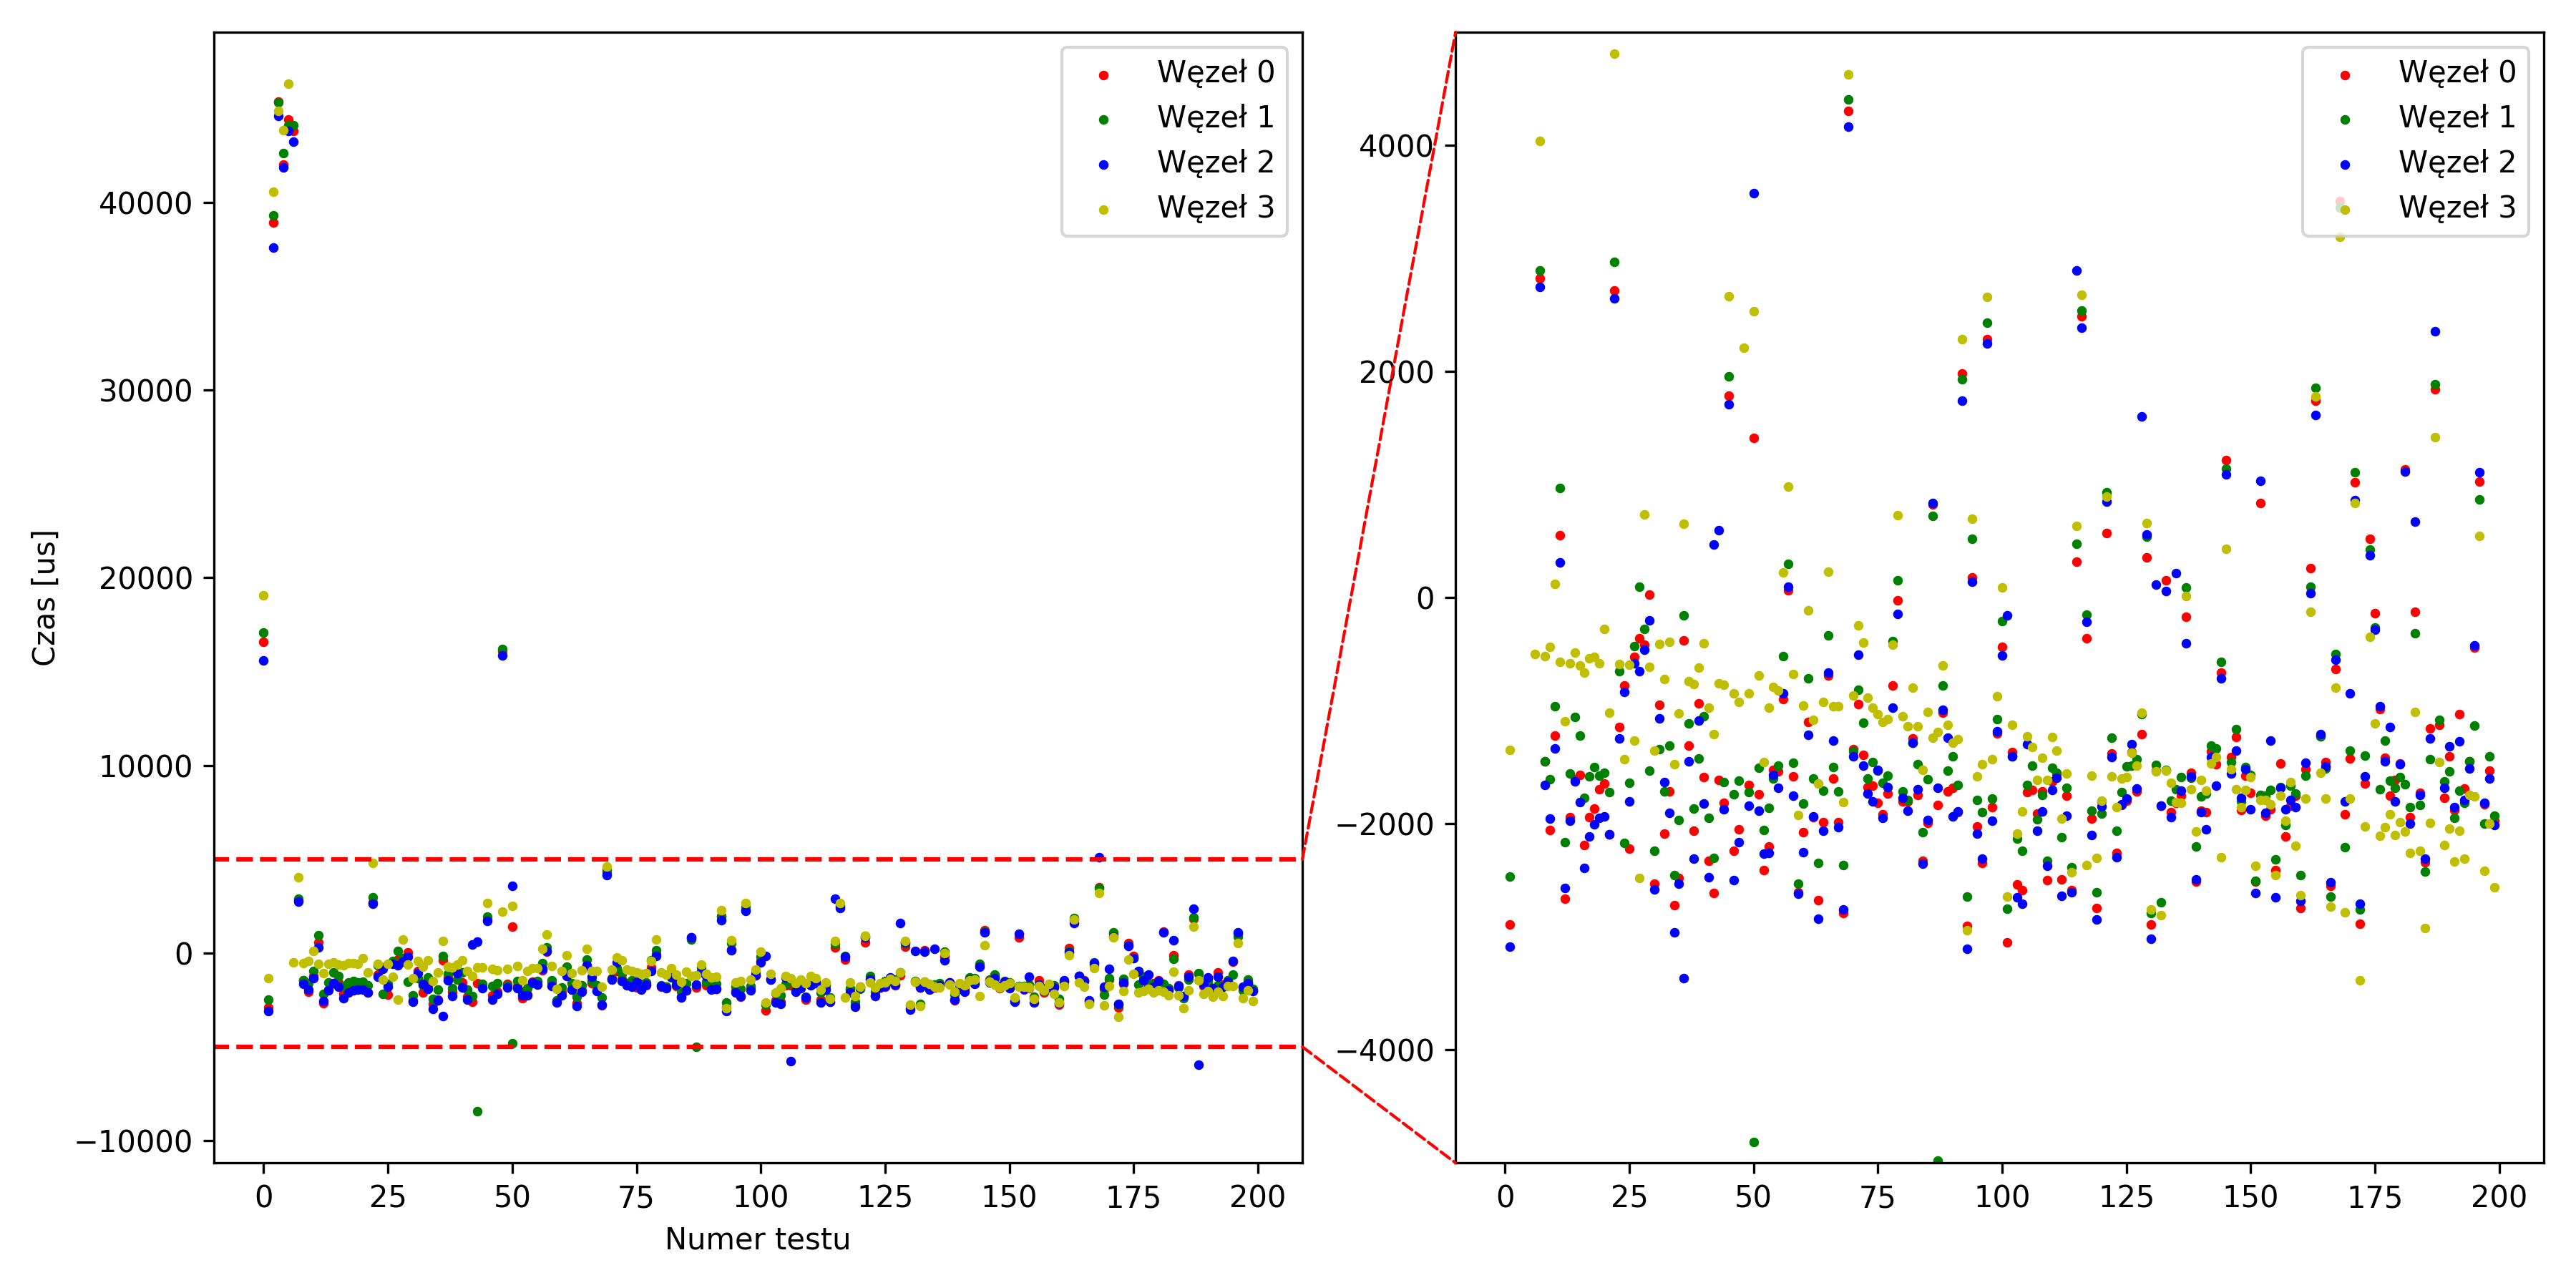
\includegraphics[width=\textwidth]{pics/ntp_sync/offsets.png}
    \caption{Wyniki pomiarów przesunięć zegarów}
    \label{pic:offsets_ntp}
\end{figure}

\begin{figure}[H]
    \centering
    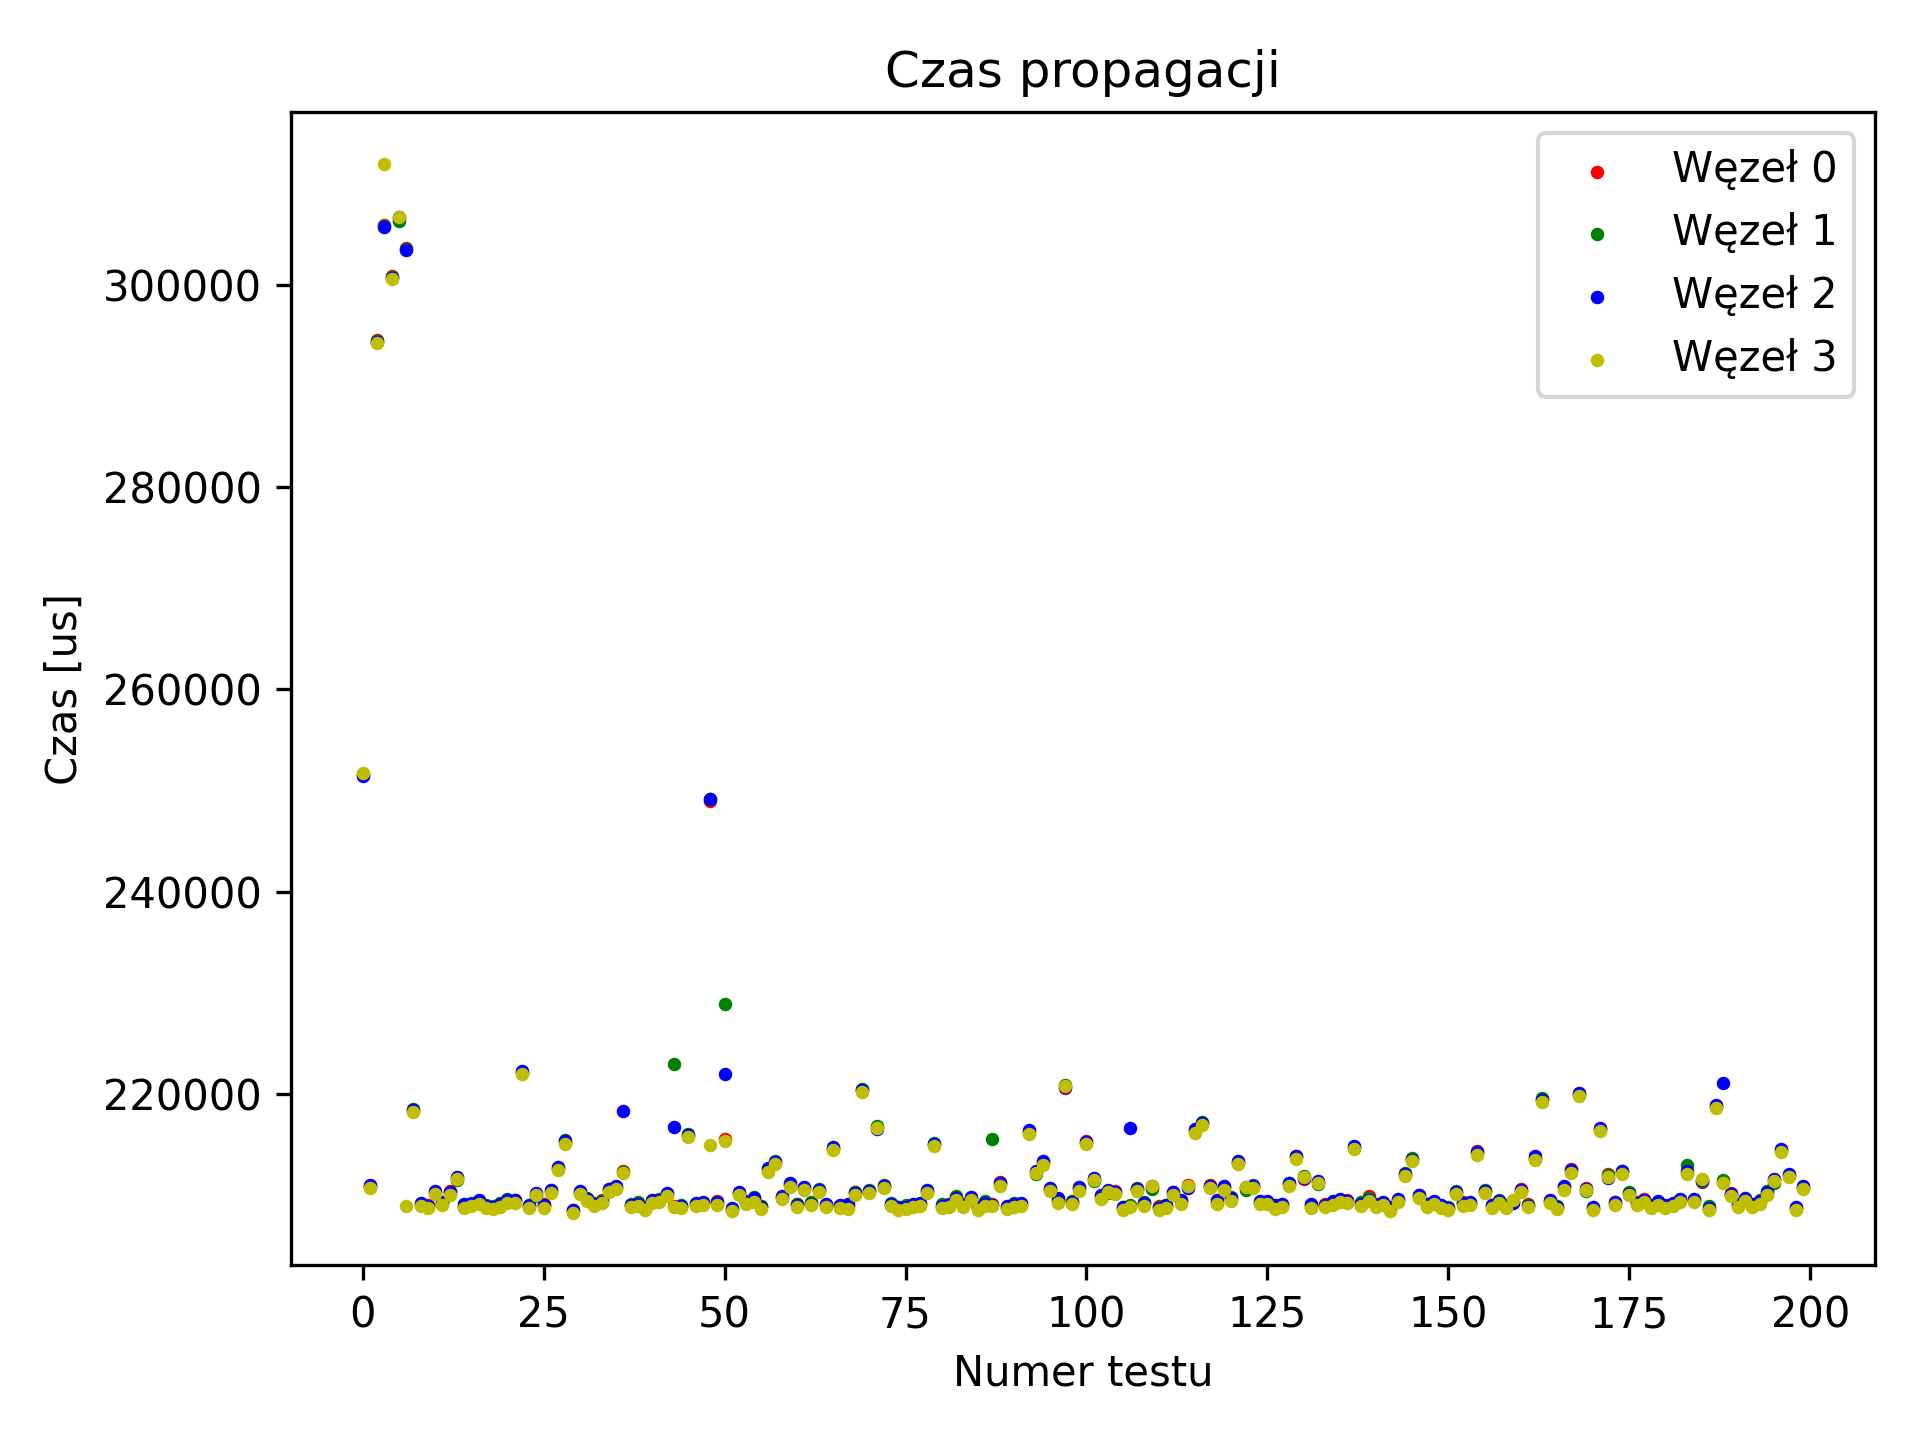
\includegraphics[width=\textwidth]{pics/ntp_sync/prop_times.png}
    \caption{Wyniki pomiarów czasów propagacji}
    \label{pic:prop_times}
\end{figure}

\begin{figure}[H]
    \centering
    \begin{subfigure}{0.5\textwidth}
        \centering
        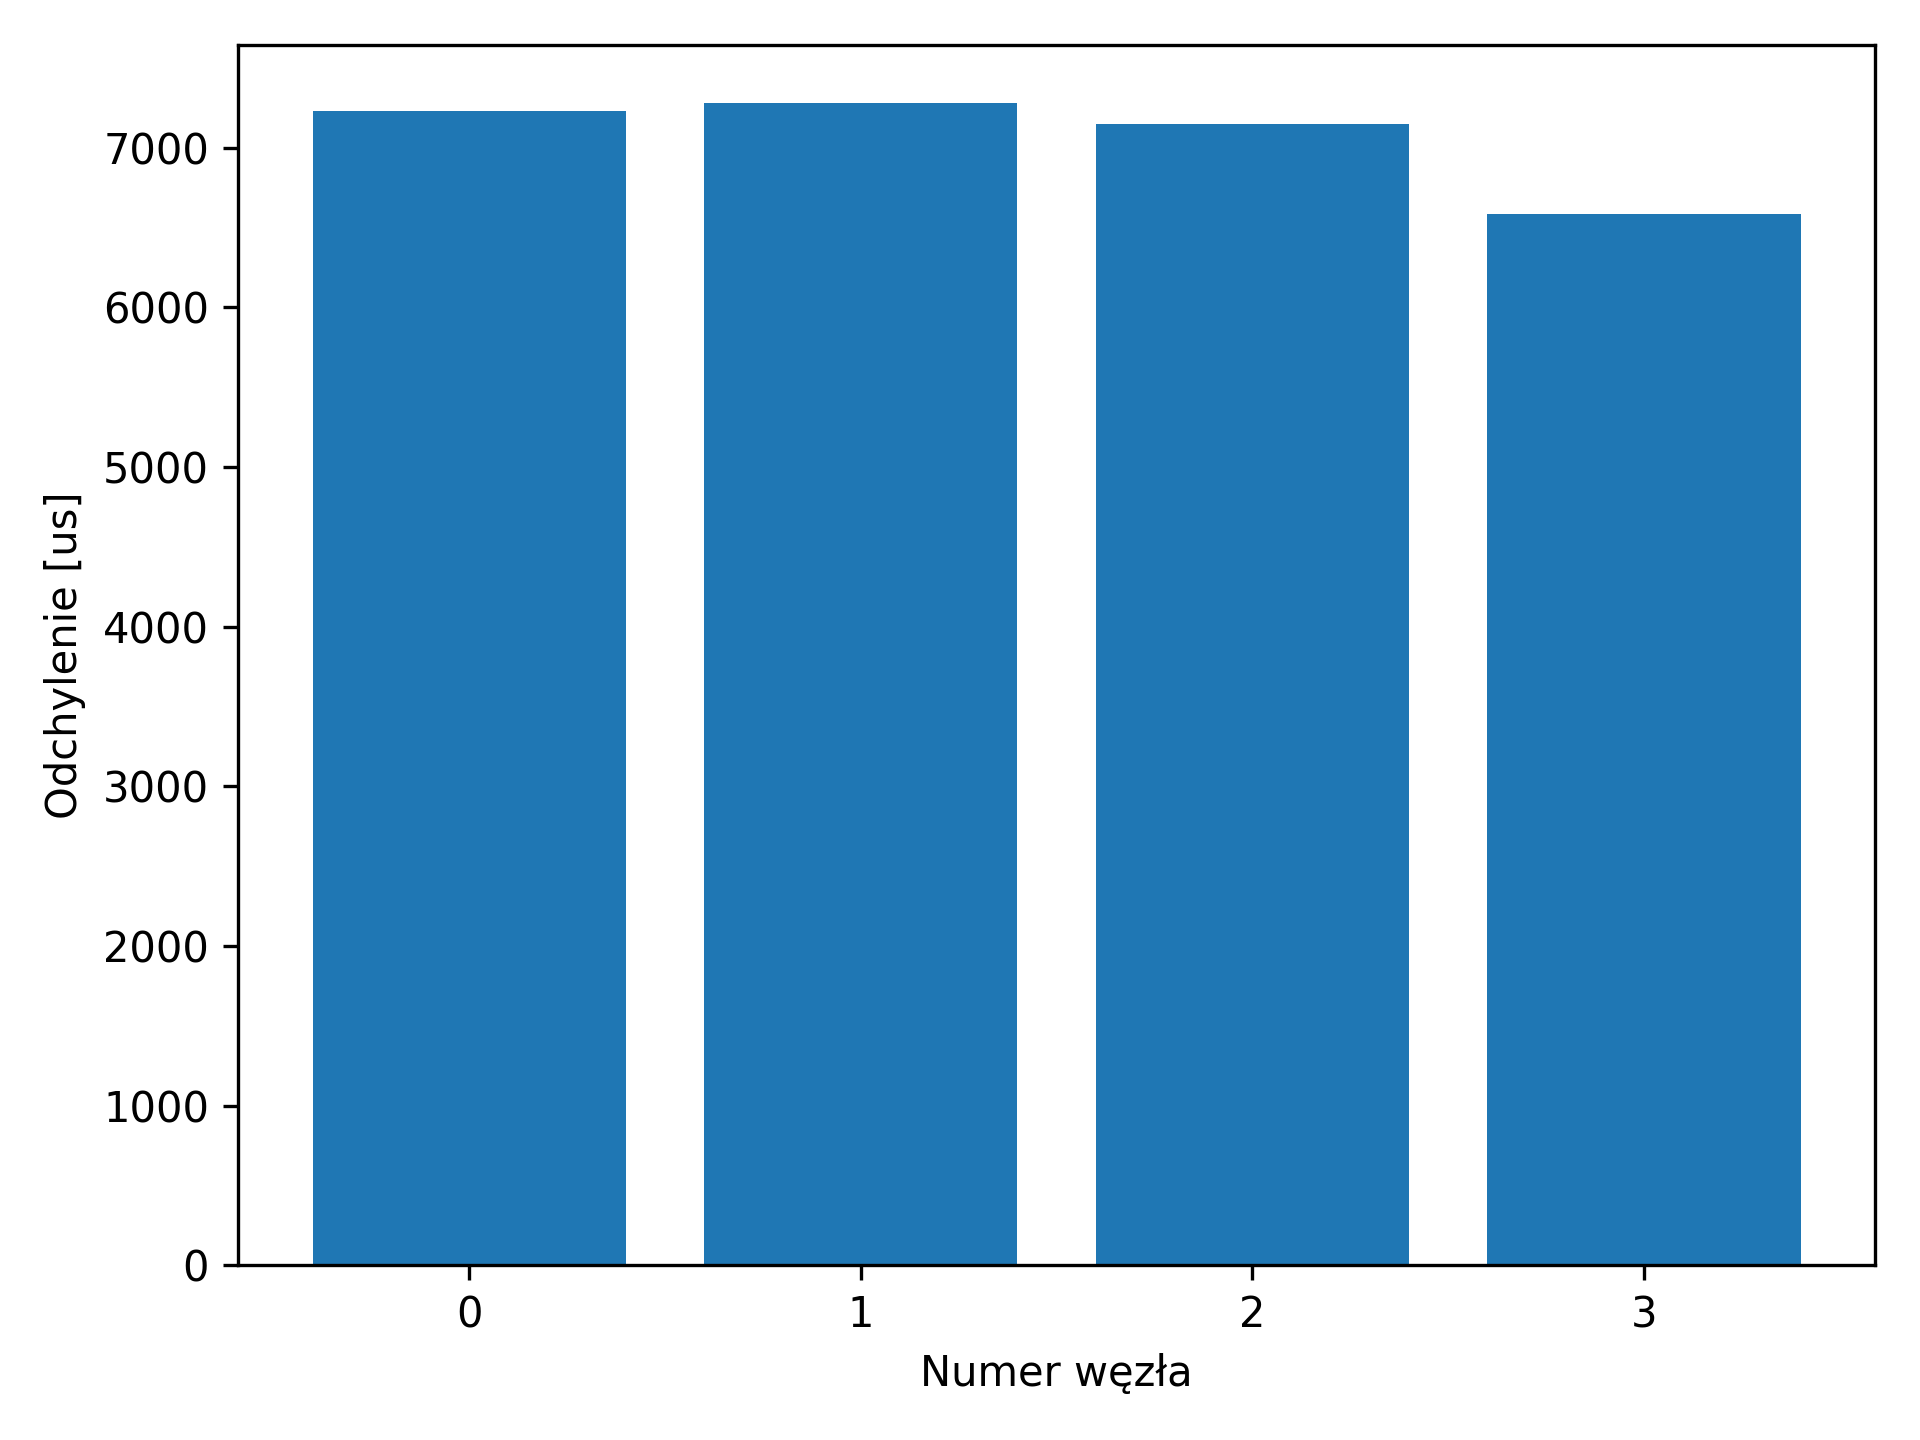
\includegraphics[width=\textwidth]{pics/ntp_sync/stddev_offsets.png}
        \caption{Odchylenia standardowe przesunięć zegarów}
        \label{pic:stddev_ntp_offsets}
    \end{subfigure}%
    \begin{subfigure}{0.5\textwidth}
        \centering
        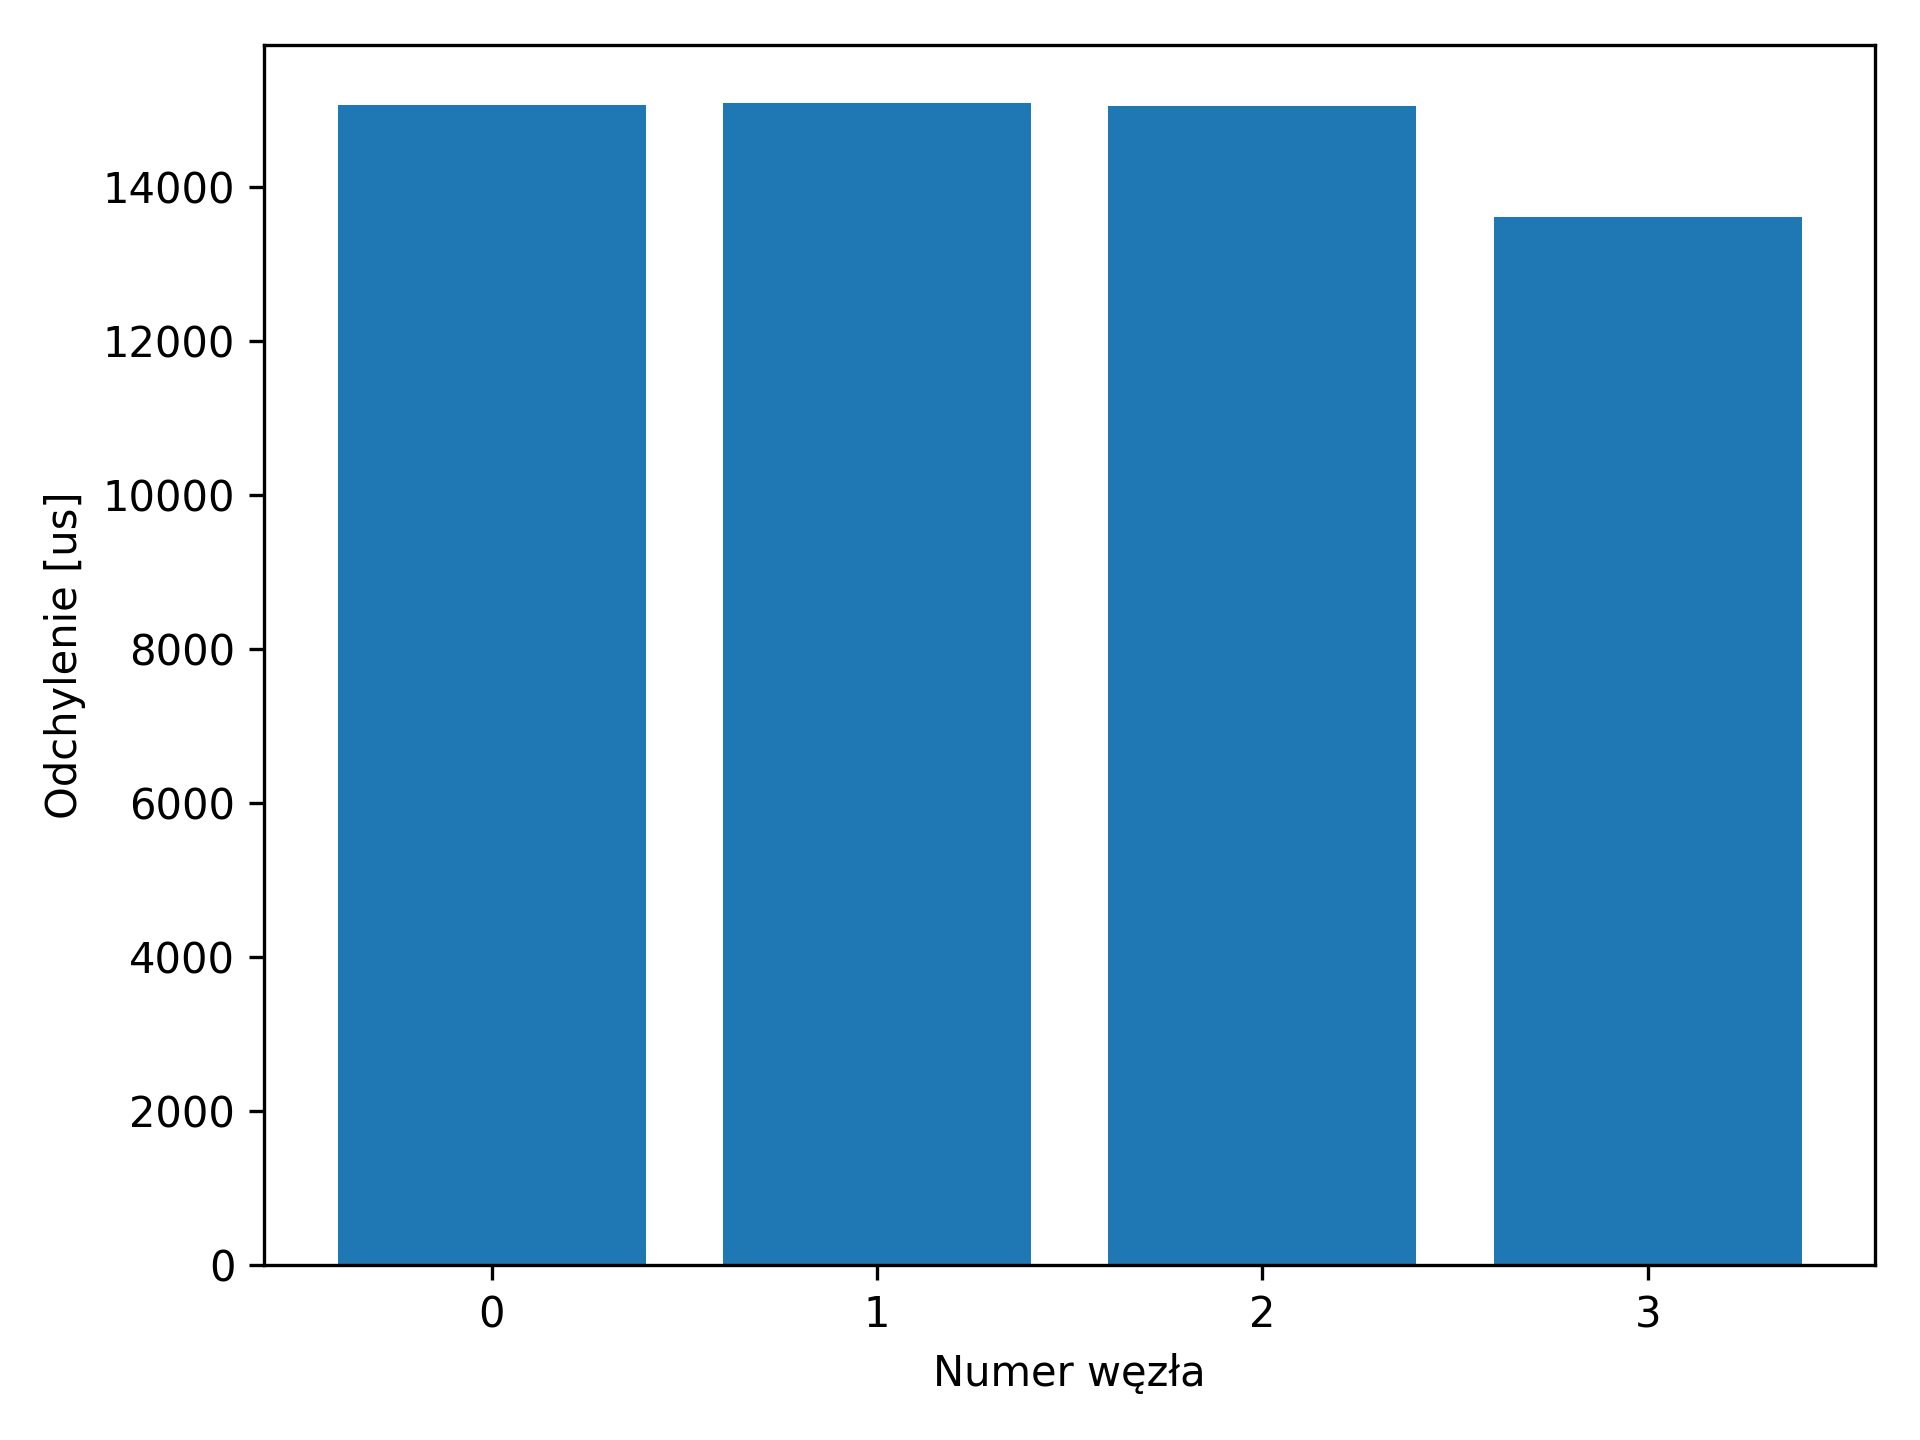
\includegraphics[width=\textwidth]{pics/ntp_sync/stddev_prop.png}
        \caption{Odchylenia standardowe czasu propagacji}
        \label{pic:stddev_ntp_prop}
    \end{subfigure}
    \caption{Odchylenia standardowe pomiarów}
    \label{fig:stddev_ntp}
\end{figure}

Na podstawie otrzymanych wykresów łatwo zauważyć, że czas propagacji wiadomości w systemie jest nieprzewidywalny i zmienia sie znacząco z pomiaru na pomiar. Interesującą nas statystyką są jednak zaobserwowane przesunięcia zegarów, bez których nie jesteśmy w stanie poprawnie ocenić odległości od źródła dźwięku. Tutaj wartości wyglądają na bardziej skoncentrowane, jednak nie widać wyraźnych tendencji koncentracji wokół wartości średnich dla żadnego z węzłów. Ponadto zaobserwowane odchylenia standardowe $\sigma_i,\ i \in \{0,1,2,3\}$ wielkości $\approx 7000 \mu s$ są nieakceptowalne, ponieważ w takim czasie dźwięk w powietrzu pokonuje $\frac{7000}{1000000}s \cdot 343\frac{m}{s} = 2.401m$. Możliwe jest, że wielokrotne powtarzanie pomiarów da zadowalającą wartość średnią, pozwalającą na centymetrową precyzję obliczanych odległości. W porównaniu z pozostałymi sposobami brane będą pod uwagę wartości uśrednione.

\subsection{Bezpośredni pomiar przesunięć zegarów}\label{sec:time_deltas_sync}

Biorąc pod uwagę zauważoną nieprzewidywalność i rozrzut czasów propagacji (spowodowanych najprawdopodobniej użyciem protokołu MQTT do przesyłu wiadomości pomiędzy urządzeniami) następnym pomysłem schematu synchronizacji jest bezpośrednie badanie względnego przesunięcia zegarów. Węzeł wysyła $n$ wiadomości zawierających aktualną wartość zegara, która po odebraniu przez serwer jest porównywana z zegarem w nim dostępnym.

\begin{figure}[H]
    \centering
    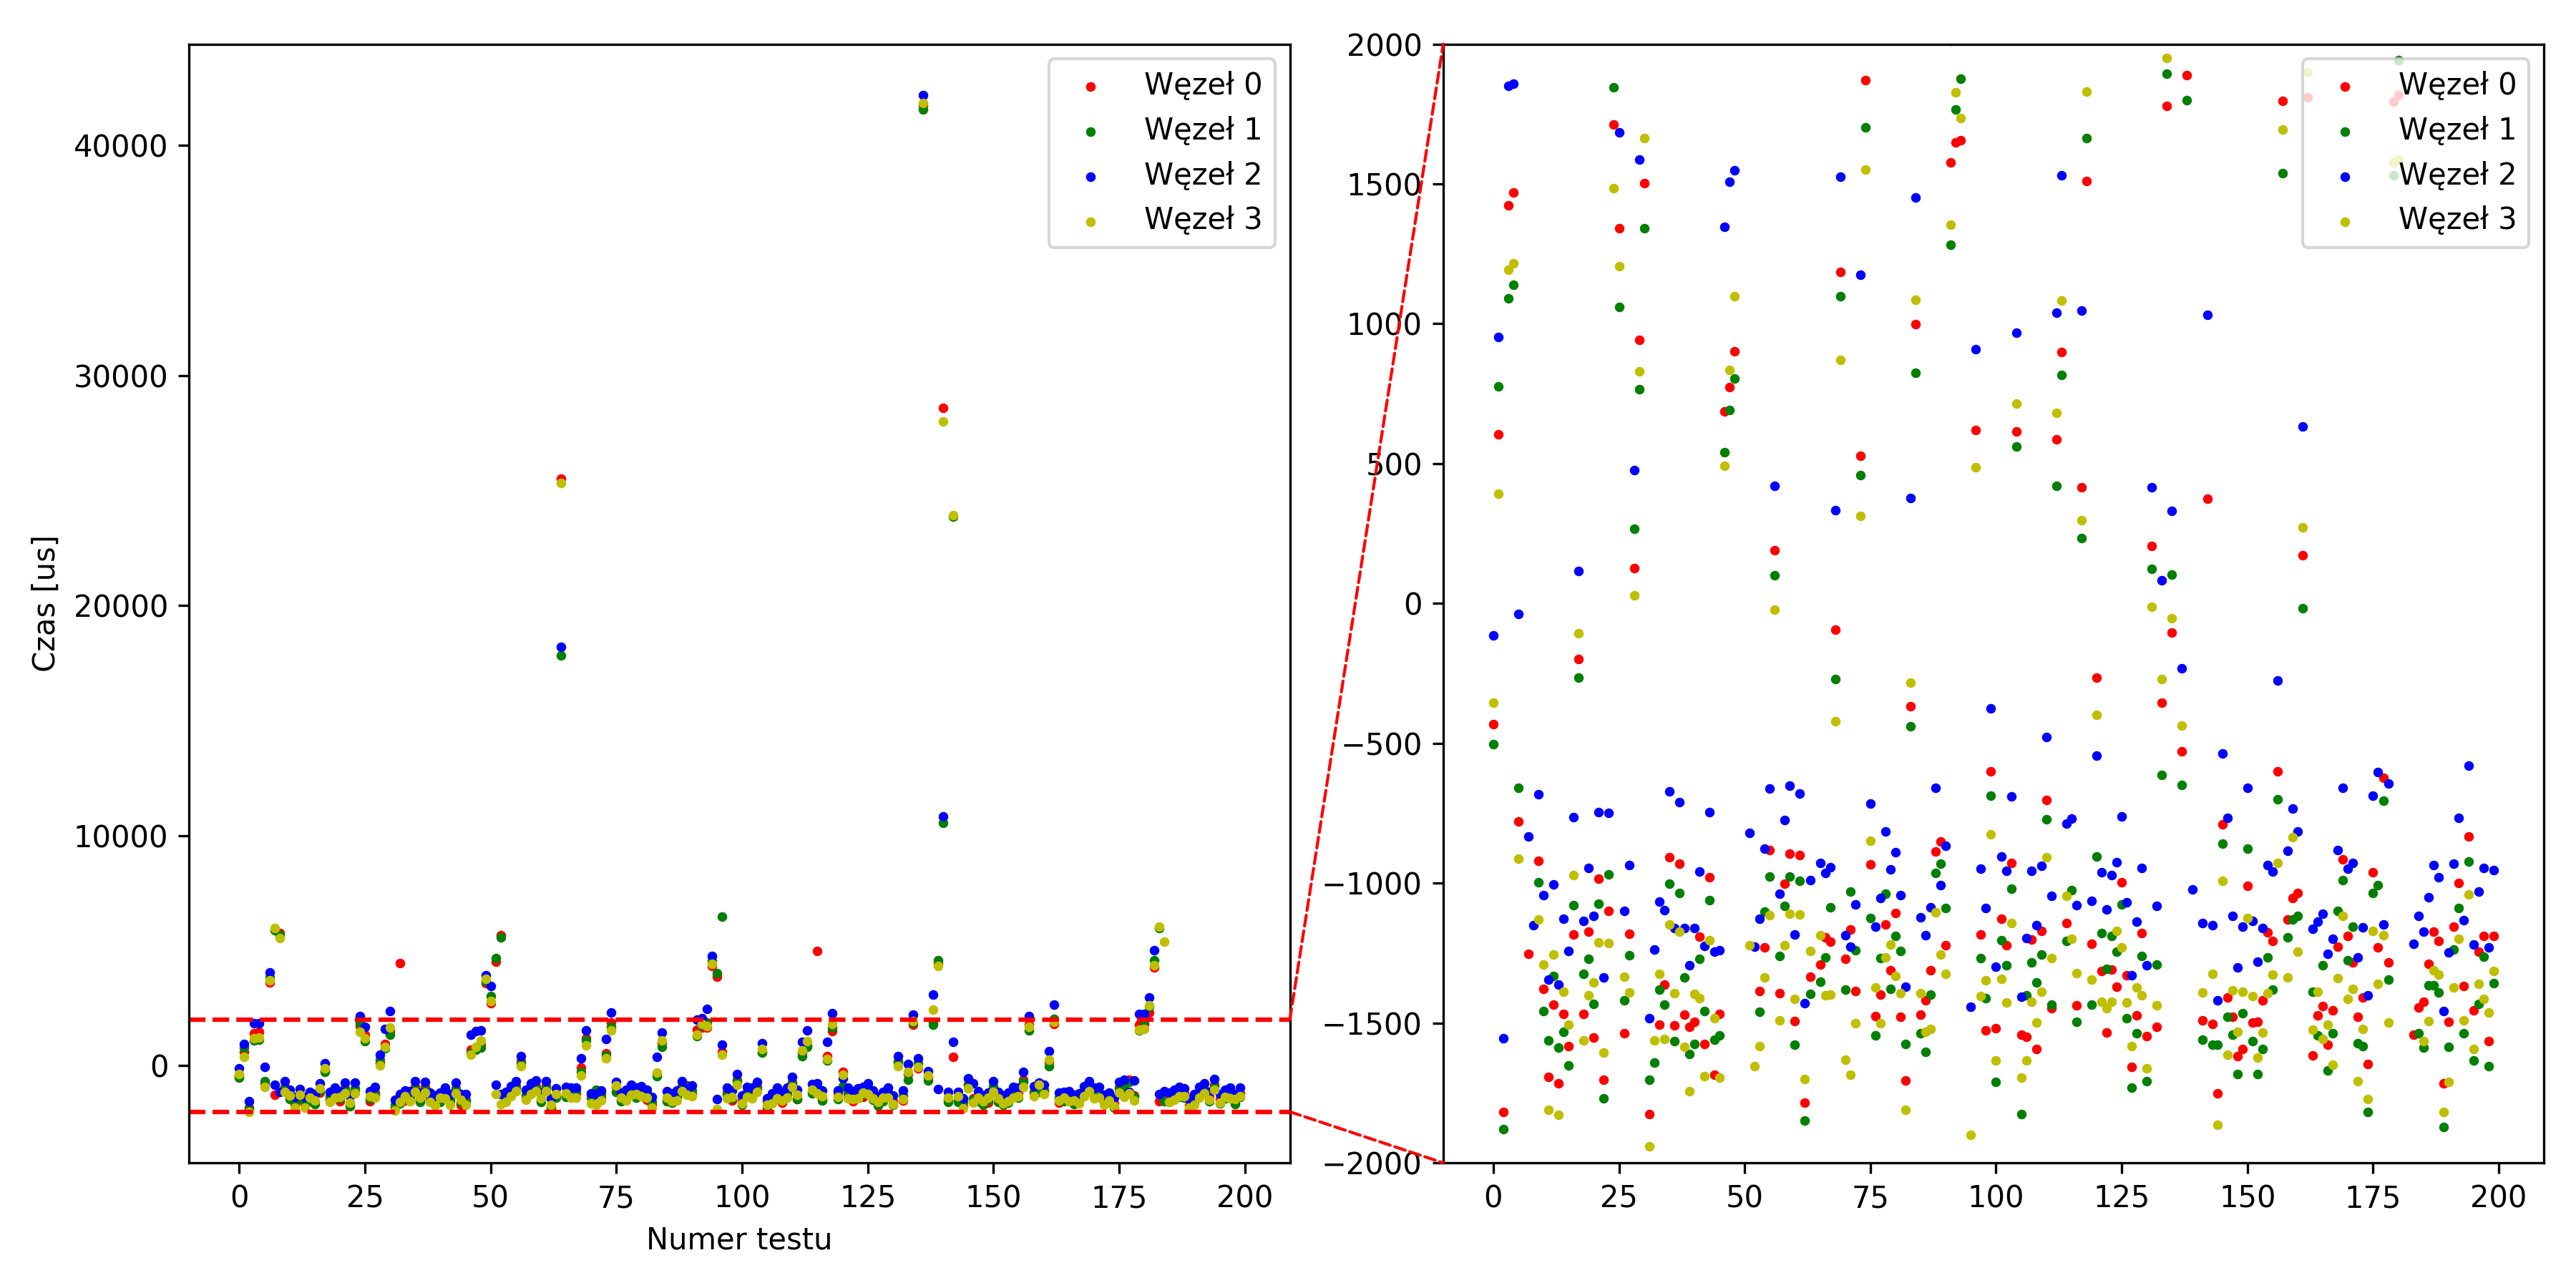
\includegraphics[width=\textwidth]{pics/time_deltas/time_deltas.png}
    \caption{Wyniki pomiarów przesunięć zegarów}
    \label{pic:offsets_deltas}
\end{figure}

\begin{figure}[H]
    \centering
    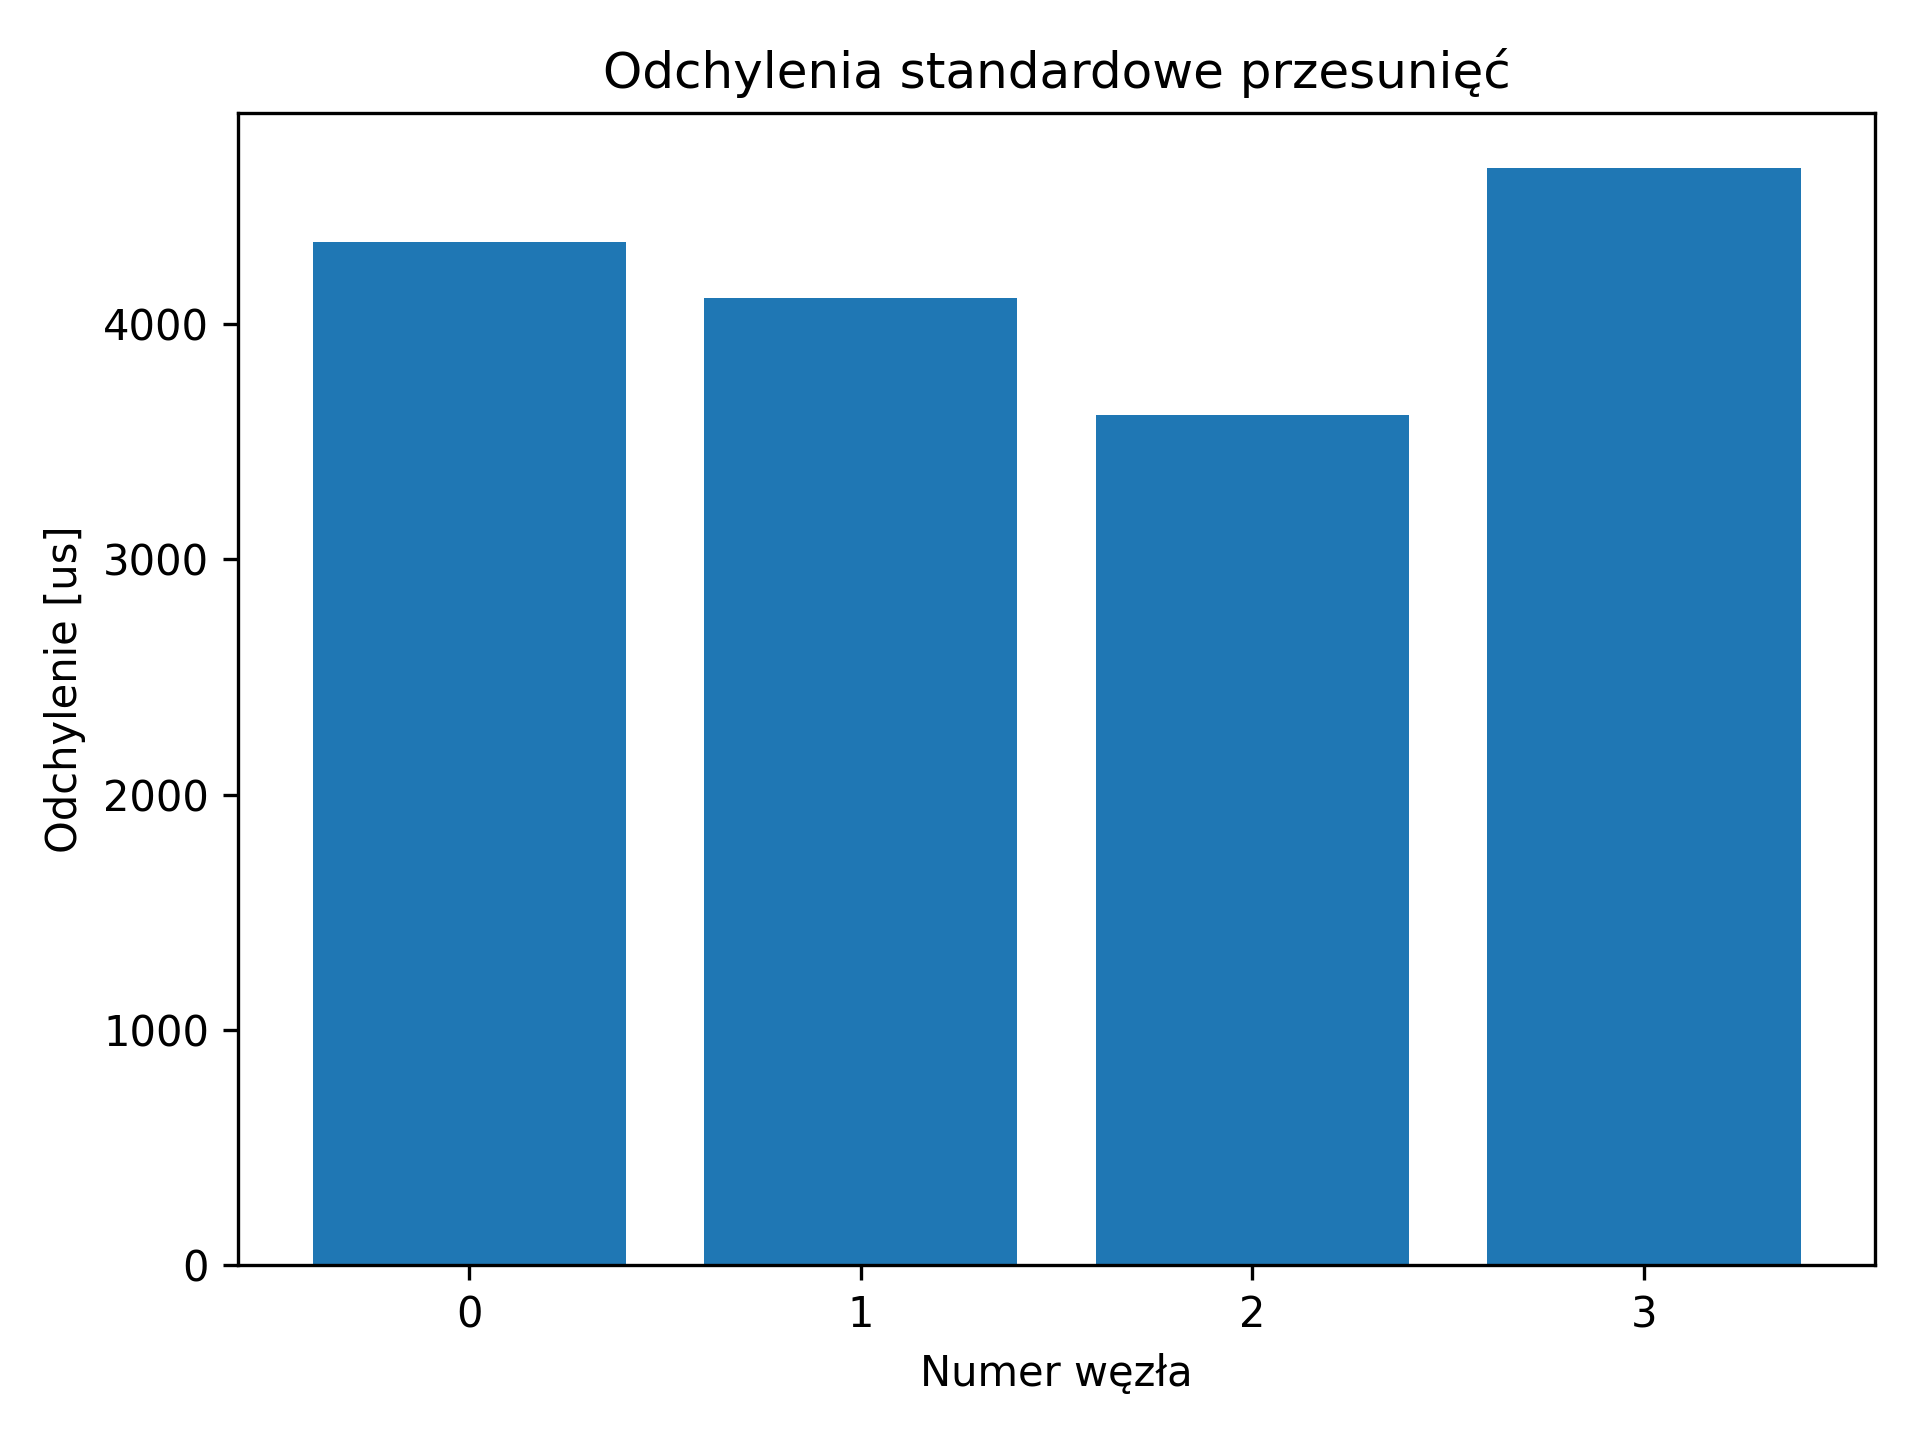
\includegraphics[width=.49\textwidth]{pics/time_deltas/stddev.png}
    \caption{Odchylenia standardowe pomiarów}
    \label{pic:stddev_deltas}
\end{figure}

Wykresy przesunięć wygenerowane na podstawie tych testów na pierwszy rzut oka są skoncentrowane podobnie jak poprzednie, jednakże odchylenie standardowe są prawie dwukrotnie mniejsze niż uprzednio, co daje nadzieje na bardziej wiarygodne wyniki. W porównaniu z pozostałymi sposobami brane będą pod uwagę wartości uśrednione.

\section{Synchronizacja sprzętowa}

TODO

\subsection{Synchronizacja z użyciem mikrofonów}\label{sec:mic_sync}

Innym pomysłem na synchronizację zegarów w węzłach było użycie mikrofonów, w które węzły odbiorcze są wyposażone. Potrzebujmy znać jedynie przesunięcie naszego zegara względem zegara w węźle nadawczym dlatego wystarczającym będzie porównanie czasu nadania i odebrania sygnału dźwiękowego. Ponadto ten rodzaj synchronizacji w przeciwieństwie do synchronizacji programowej, która uzgadniała ze sobą jedynie zegary na podstawie wymienianych wiadomości, wlicza w czas transmisji wszelkie nie wzięte wcześniej pod uwagę opóźnienia, takie jak:

\begin{itemize}
    \item Czas pomiędzy wysłaniem wiadomości o nadaniu sygnału a zamknięciem kontaktora i poruszeniem membraną brzęczyka,
    \item Czas pomiędzy odebraniem sygnału przez mikrofon a zmianą stanu zmiennej na to wskazującej.
\end{itemize}

Przeprowadzono testy tego typu synchronizacji, których wyniki przedstawiono na wykresach~\ref{pic:mic_sync}. W celu zwiększenia czytelności odrzucono pierwszy z pomiarów oraz przesunięto wyniki o wartość średnią.

\begin{figure}[H]
    \centering
    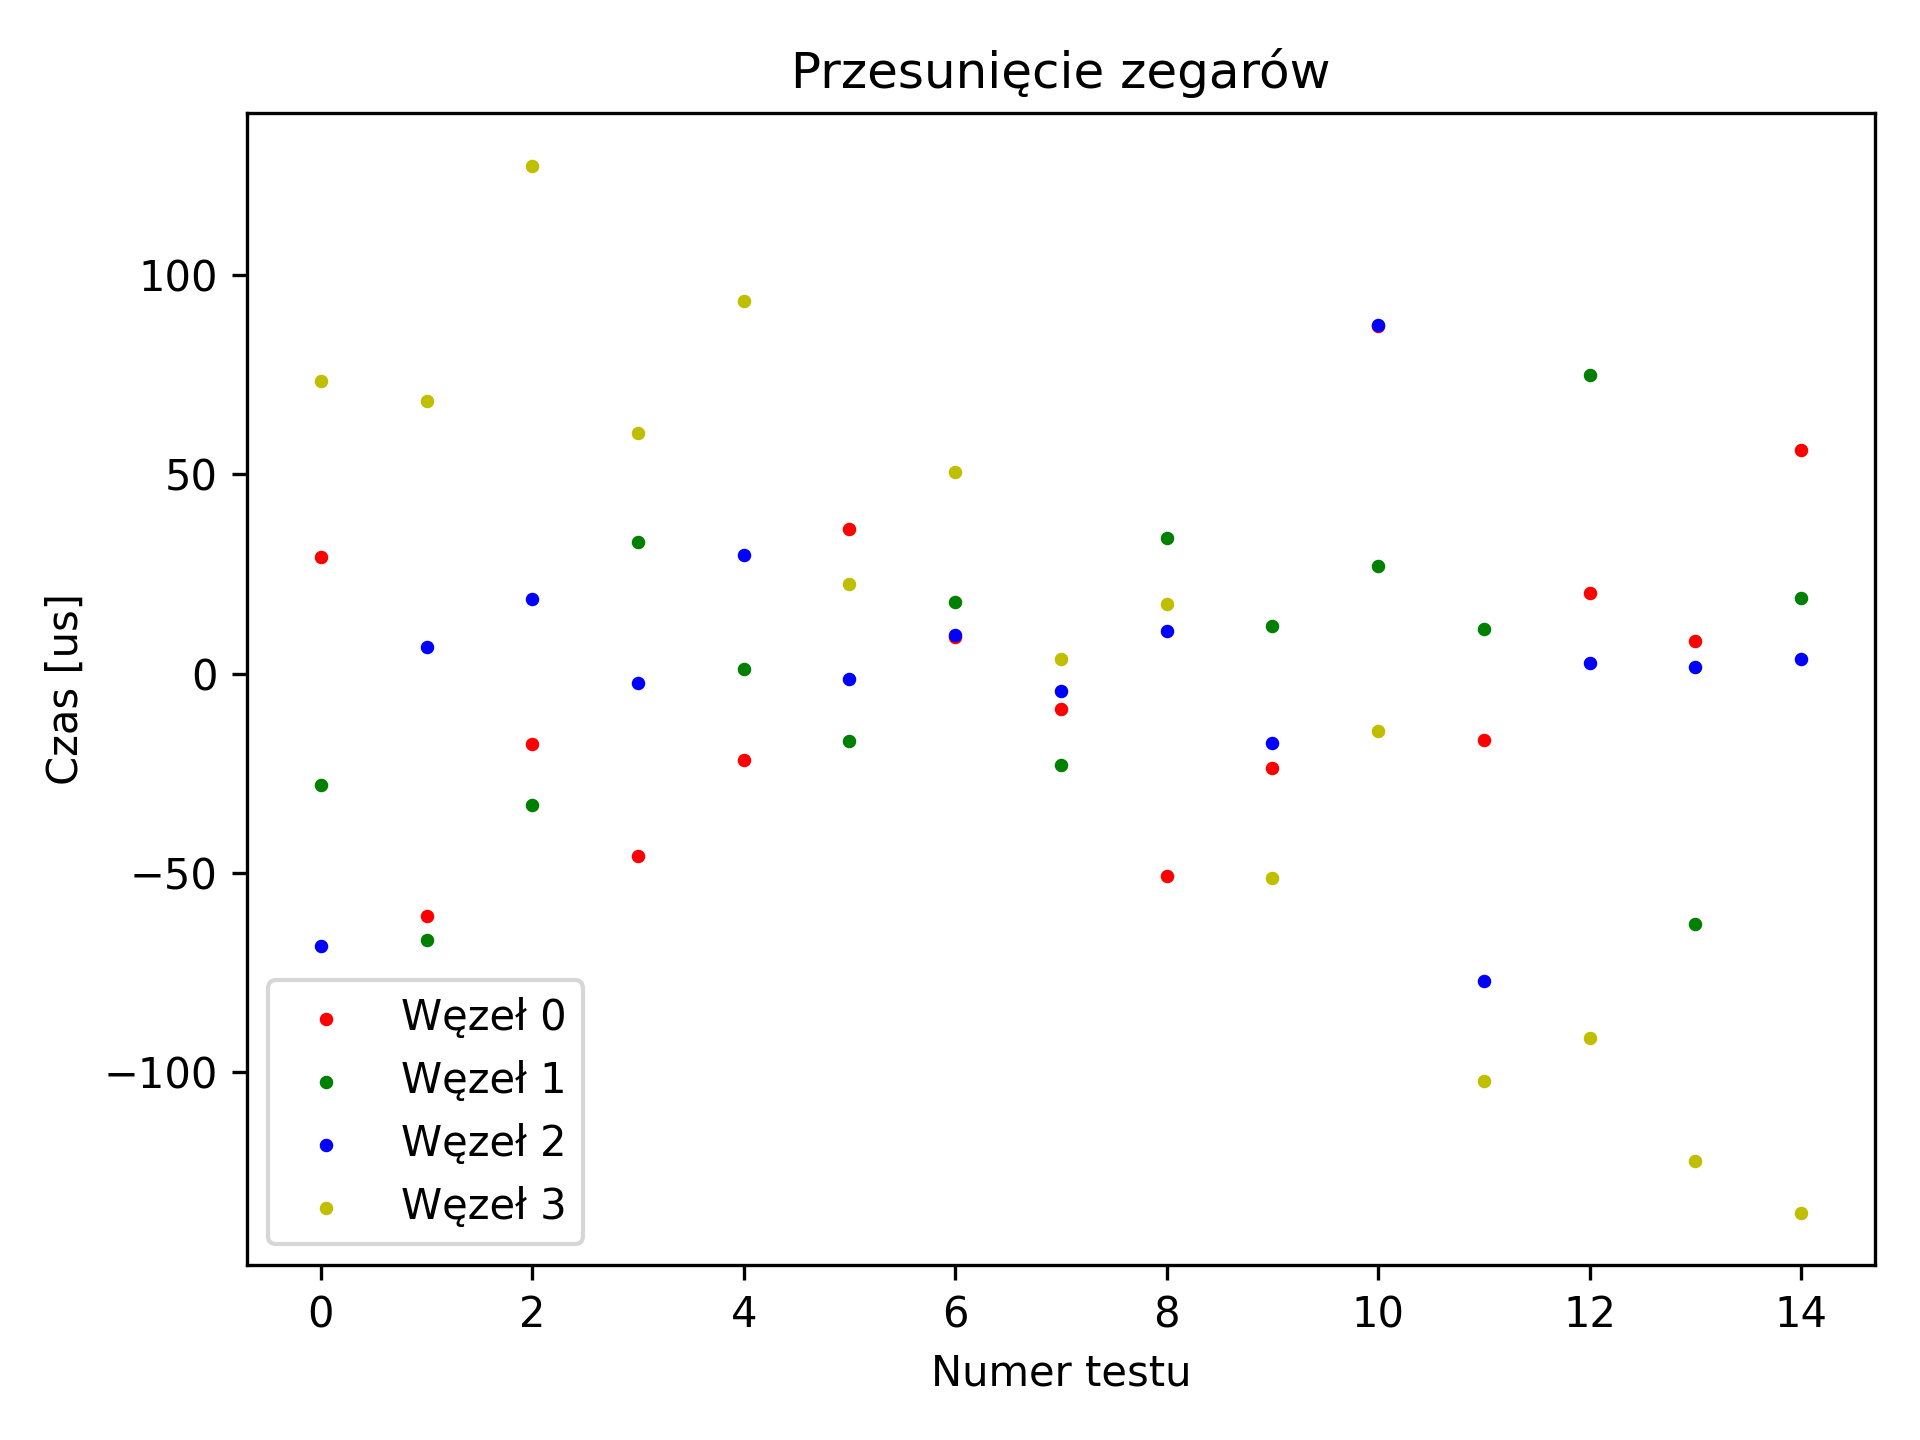
\includegraphics[width=\textwidth]{pics/mic_sync/offsets.png}
    \caption{Wyniki pomiarów przesunięć zegarów}
    \label{pic:mic_sync}
\end{figure}

\begin{figure}[H]
    \centering
    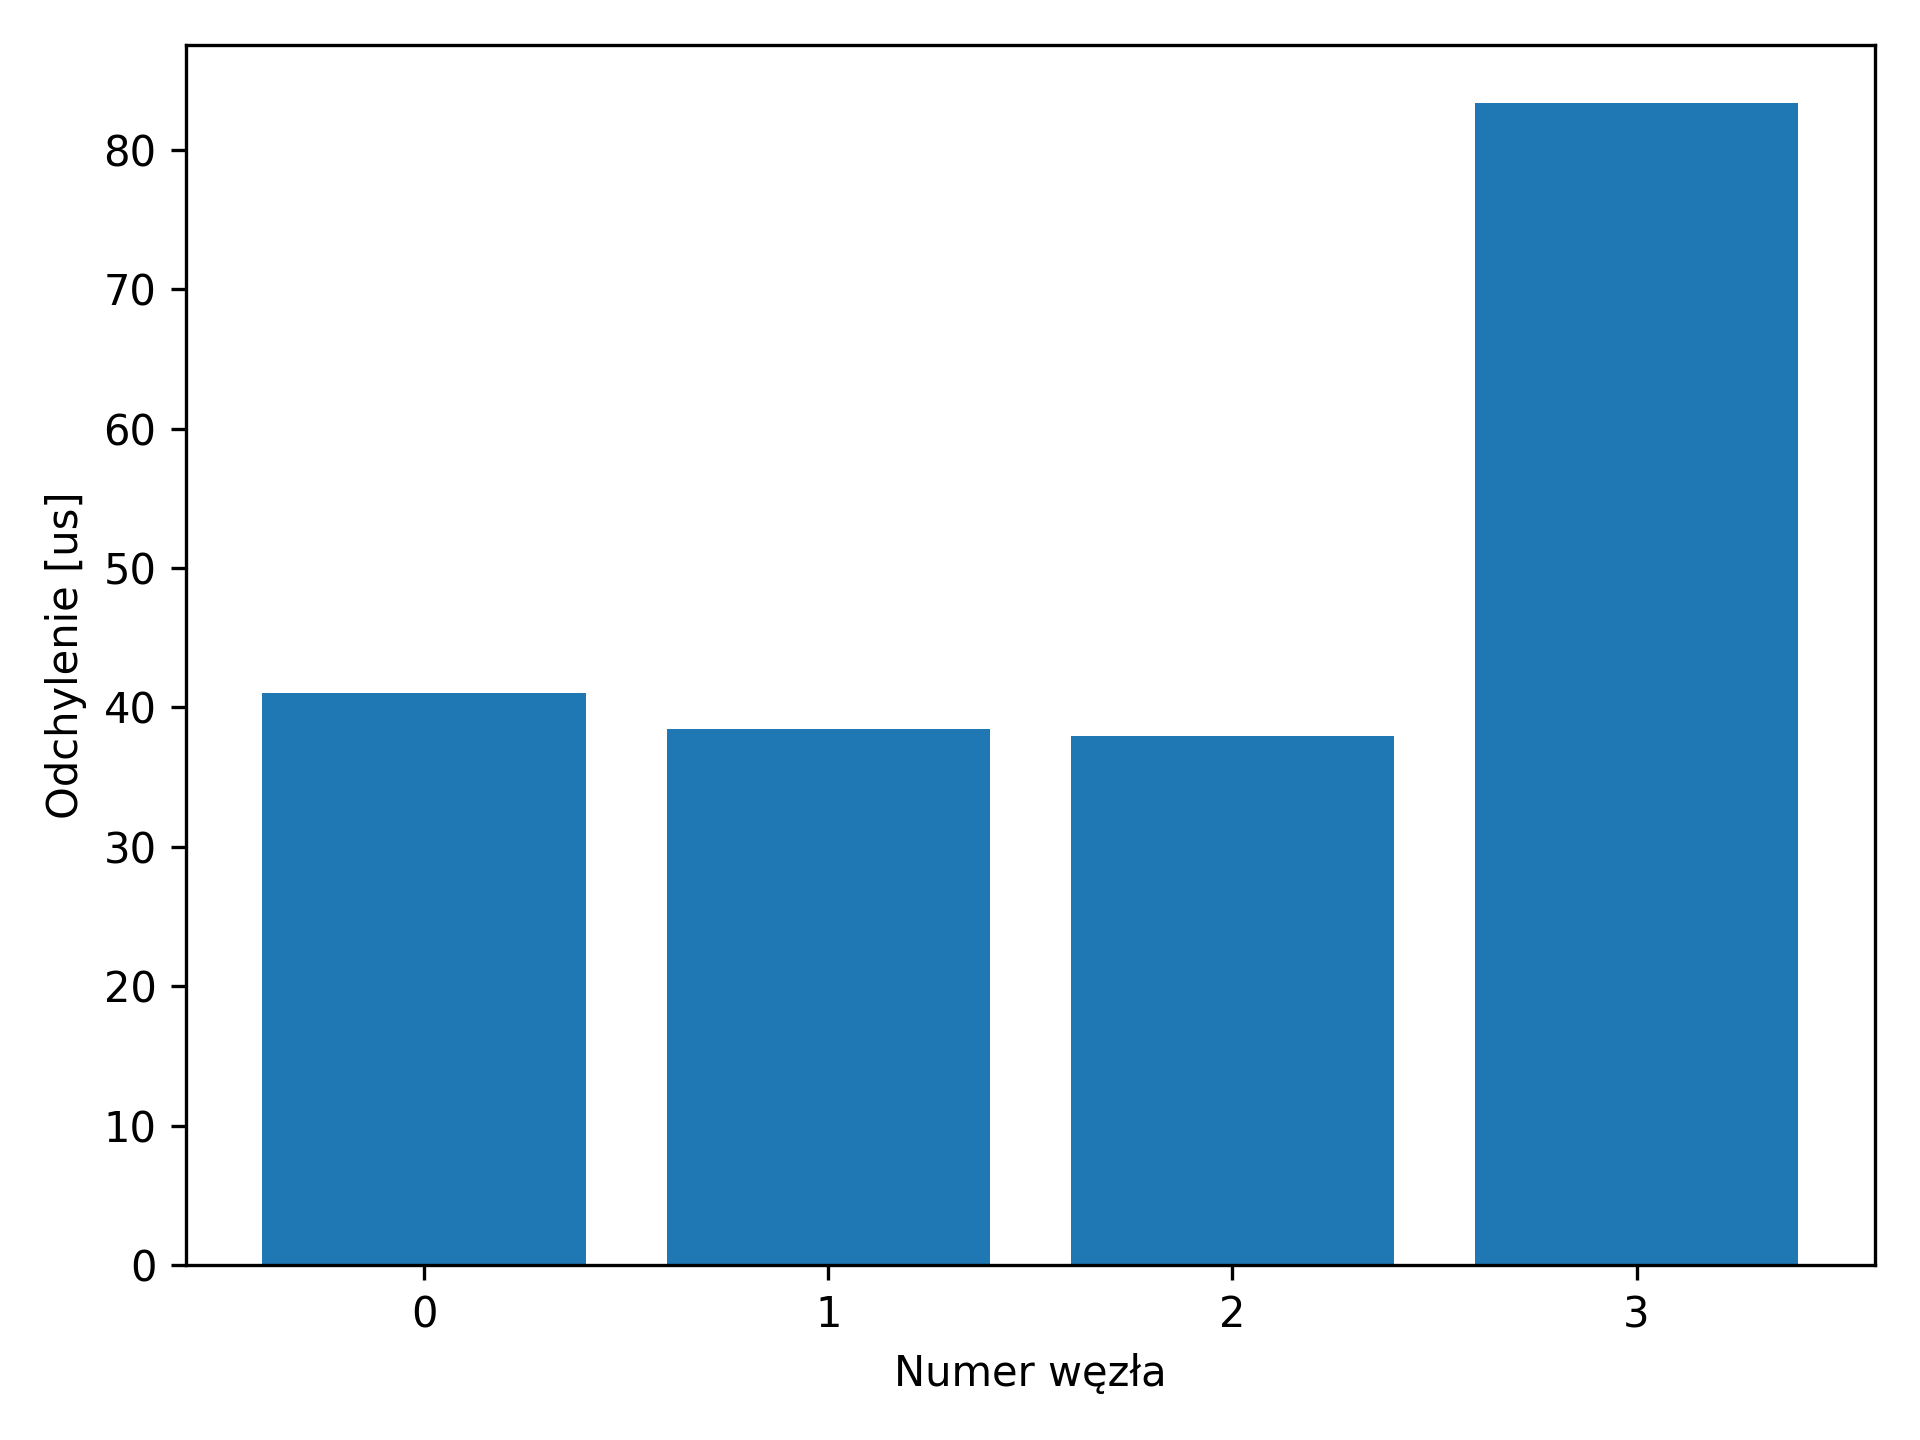
\includegraphics[width=.49\textwidth]{pics/mic_sync/stddev_offsets.png}
    \caption{Odchylenia standardowe pomiarów}
    \label{pic:stddev_mic}
\end{figure}

Łatwo zauważyć, ża udało się zmniejszyć odchylenia obliczonych przesunięć zegara aż o dwa rzędy wielkości. Taka dokładność daje znacznie lepsze przybliżenie rzeczywistej odległości między węzłami, ponieważ w czasie $40 \mu s$ dźwięk pokona jedynie $\frac{40}{10000000}s \cdot 343 \frac{m}{s} \approx 0,014m$. Mając tak dokładne odległości będziemy mogli wprowadzić je do modelu multilateracyjnego.

\subsection{Porównanie metod}

Porównajmy teraz dokładność obliczanych odległości na podstawie interwału czasowego pomiędzy nadaniem dźwięku a jego odbiorem w różnych wariantach synchronizacji zegarów. Wykresy uzyskane przy zastosowaniu synchronizacji czasowej zostały przedstawione przed i po znormalizowaniu poprzez przesunięcie tak, by średnia pomiarów rozpoczynała się od 0. Pomiary oparte o synchronizację z użyciem mikrofonów nie wymagały tego dodatkowego kroku.

\begin{figure}[H]
    \centering
    \begin{subfigure}{\textwidth}
        \centering
        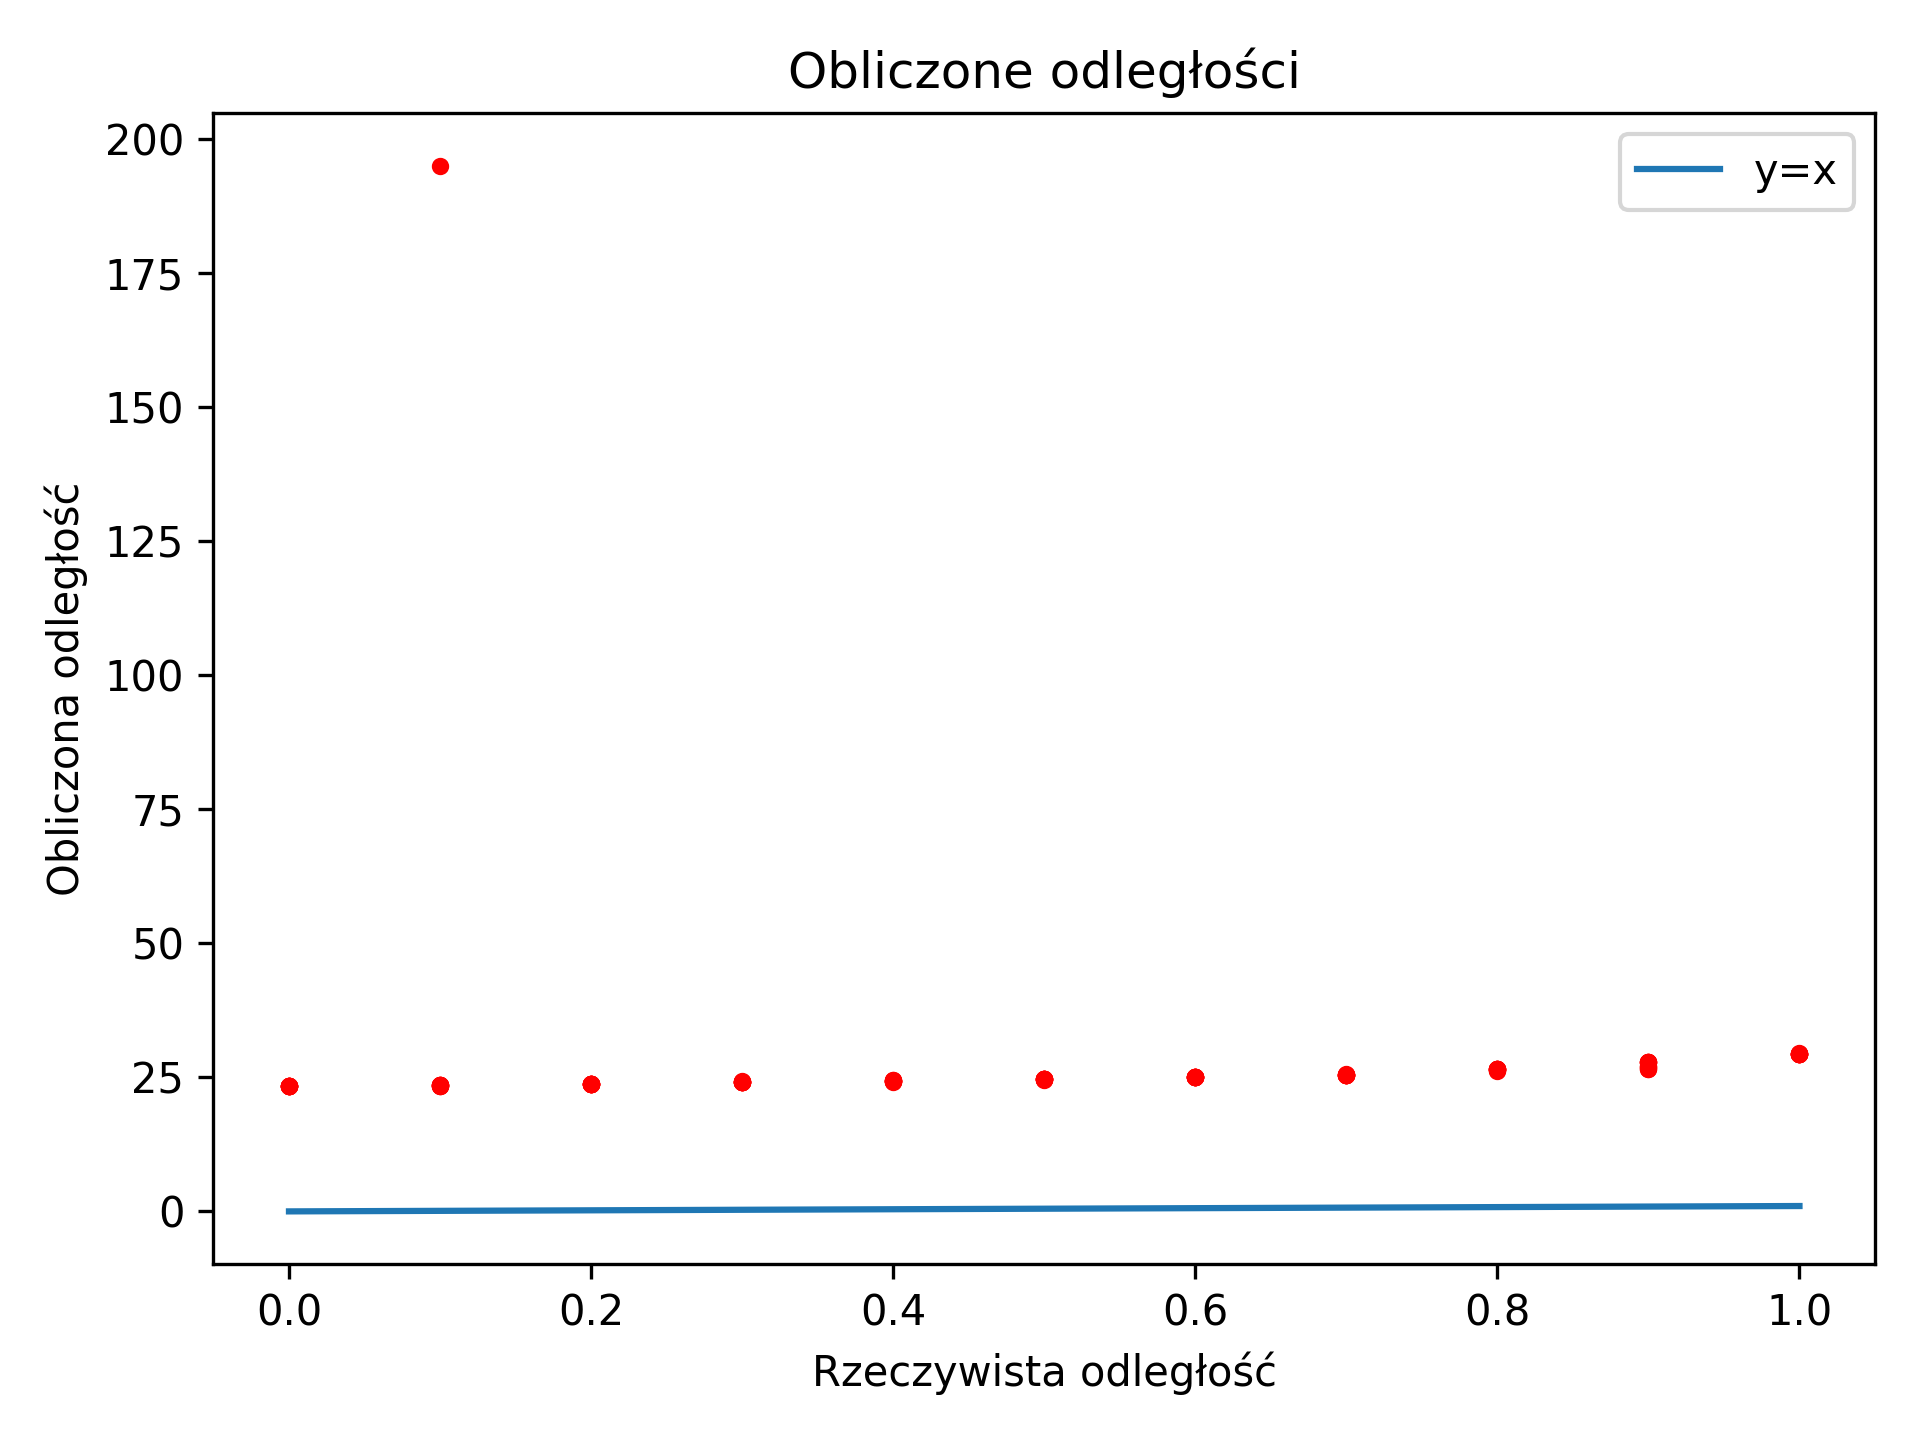
\includegraphics[width=0.49\textwidth]{pics/ntp_sync_dist/dists.png}
        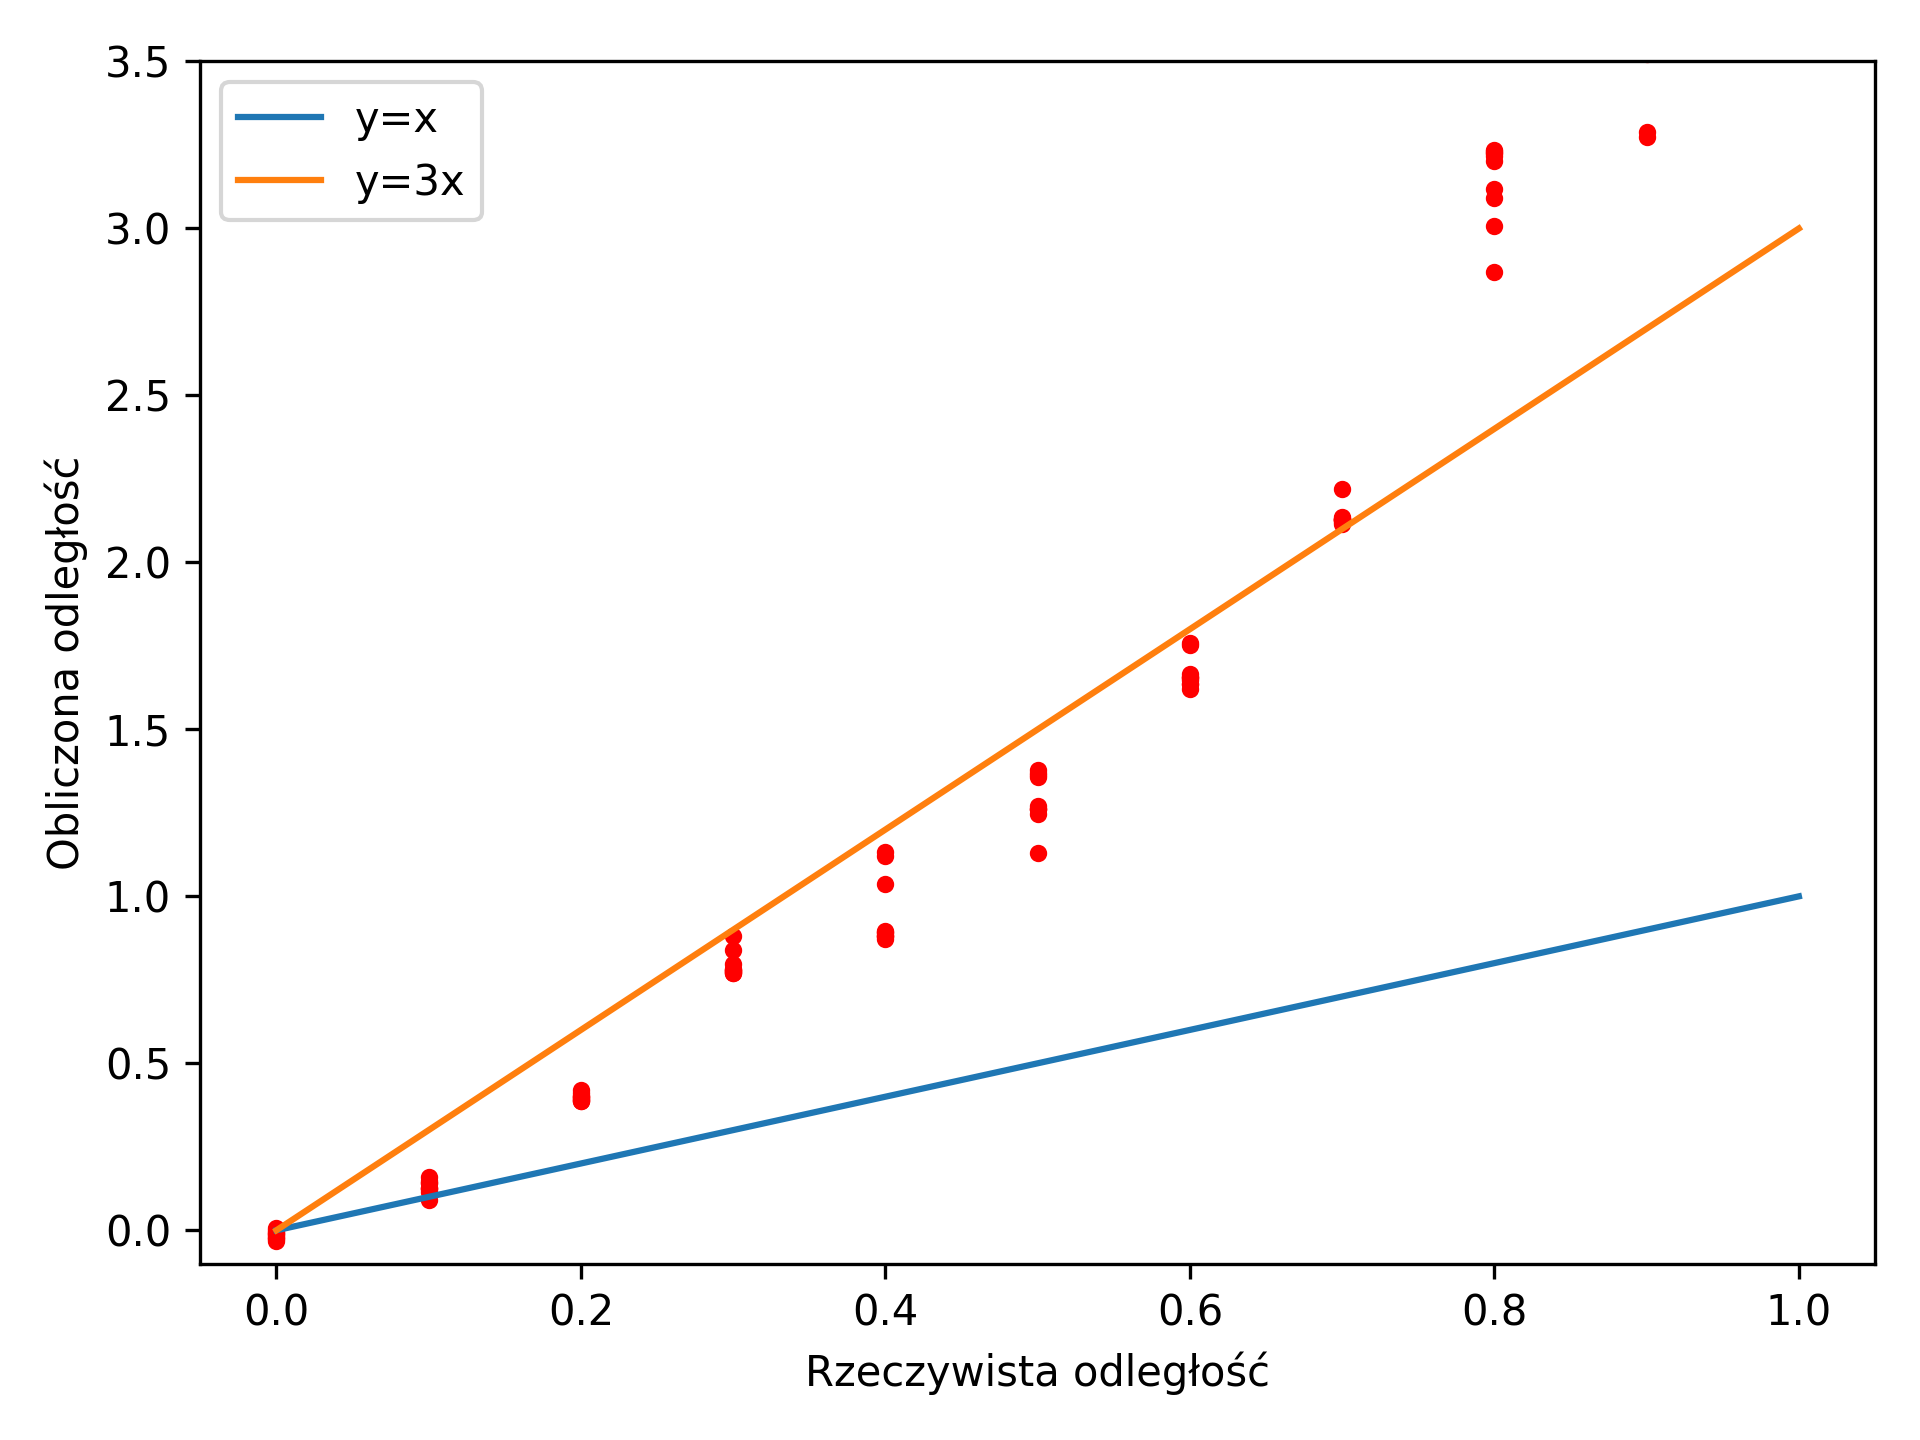
\includegraphics[width=0.49\textwidth]{pics/ntp_sync_dist/dists_close.png}
        \caption{synchronizacja NTP~\ref{sec:ntp_sync}}
        \label{pic:ntp_sync_dist}
    \end{subfigure}
\end{figure}
\begin{figure}[H]
    \ContinuedFloat\centering
    \begin{subfigure}{\textwidth}
        \centering
        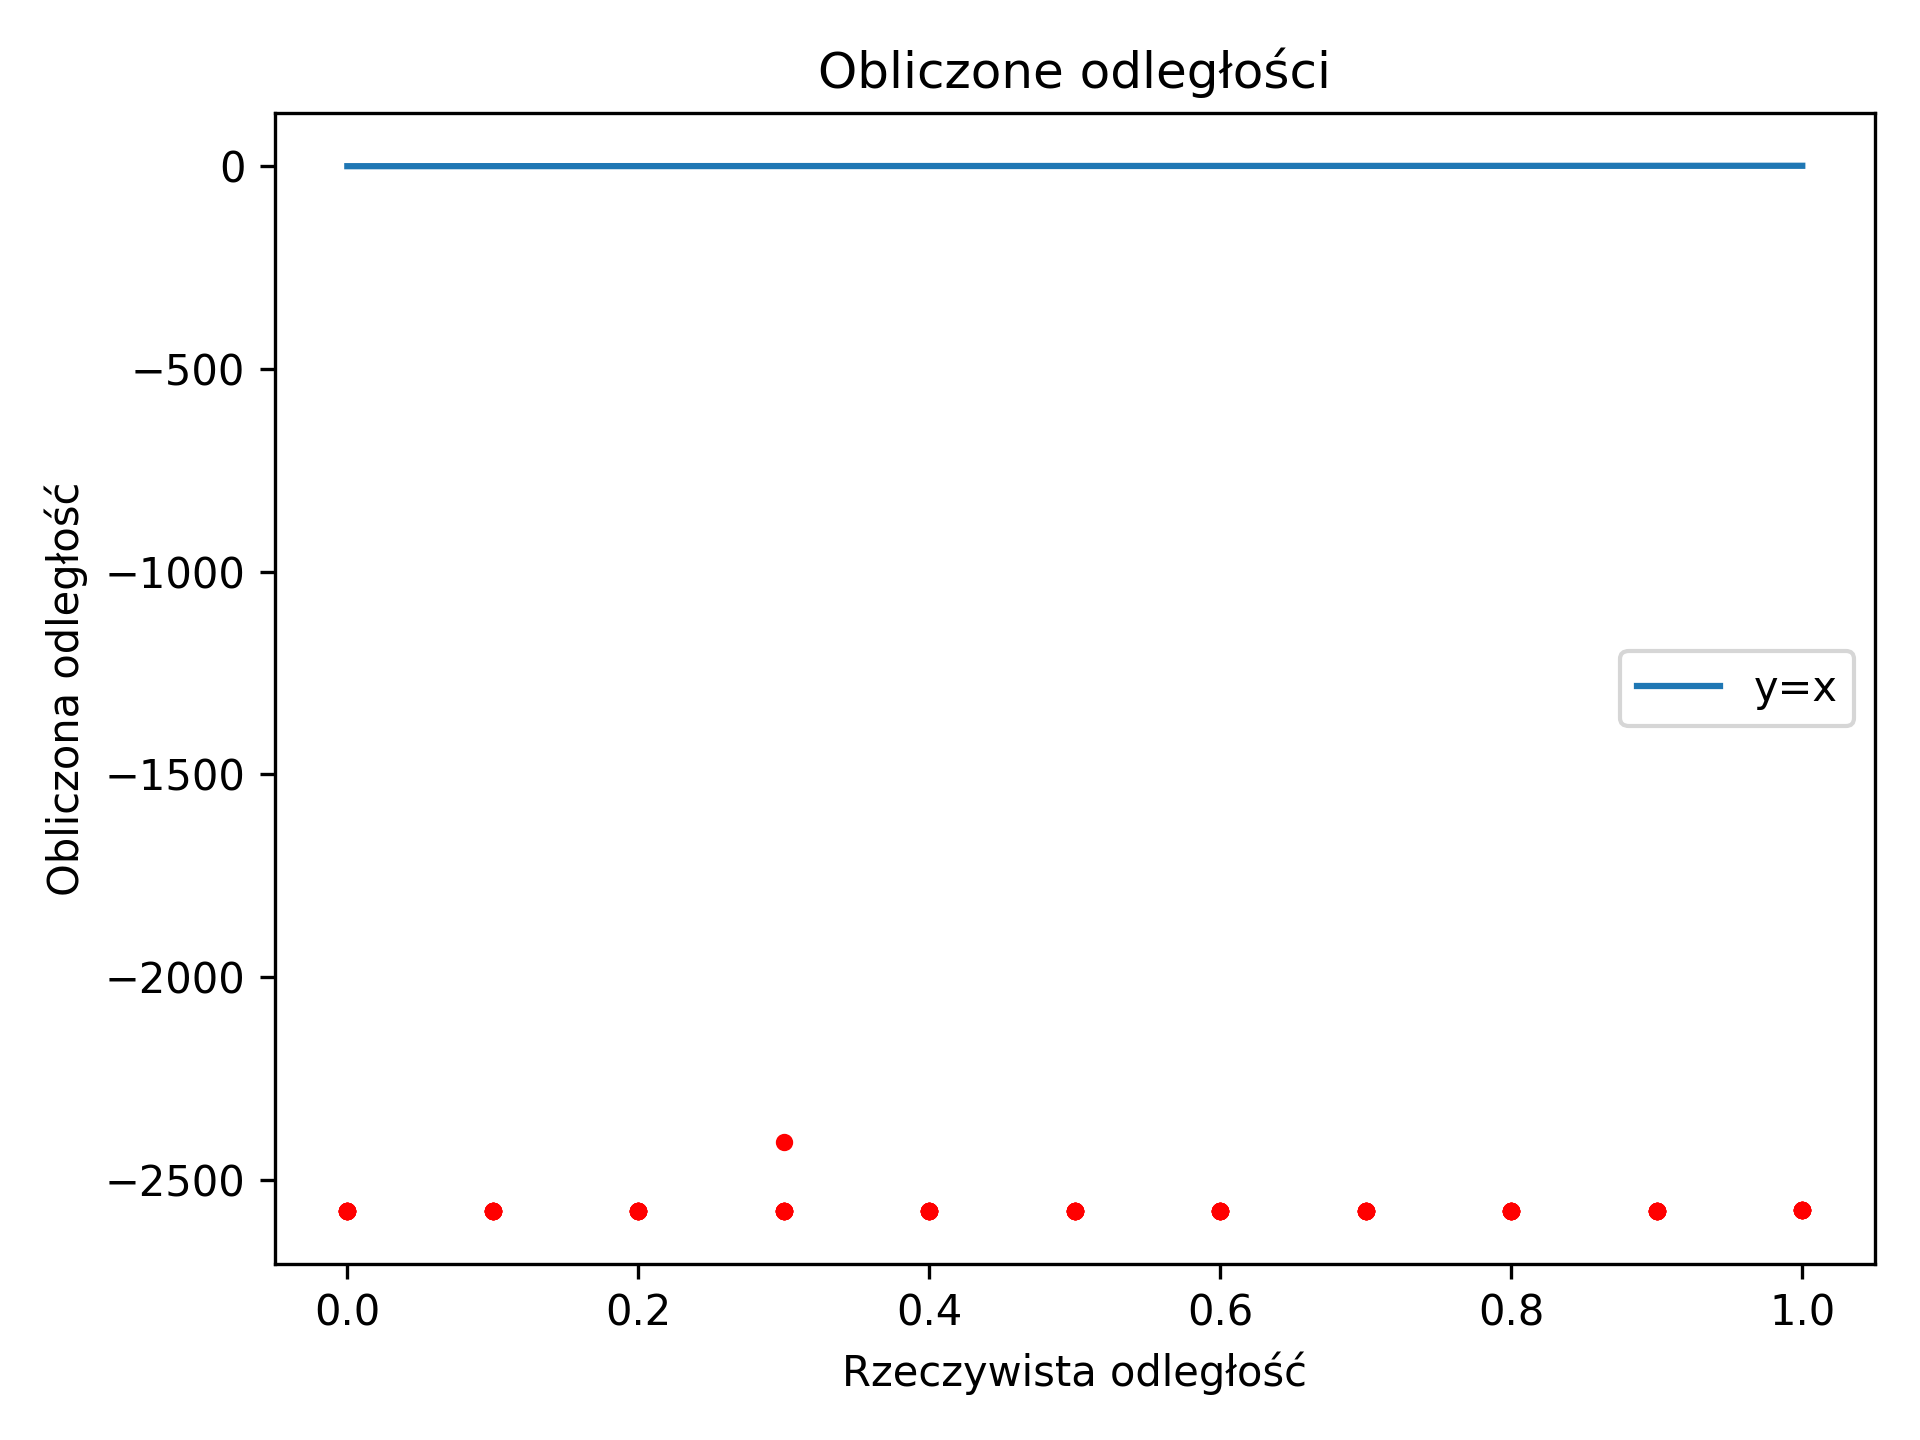
\includegraphics[width=0.49\textwidth]{pics/time_deltas_dist/dists.png}
        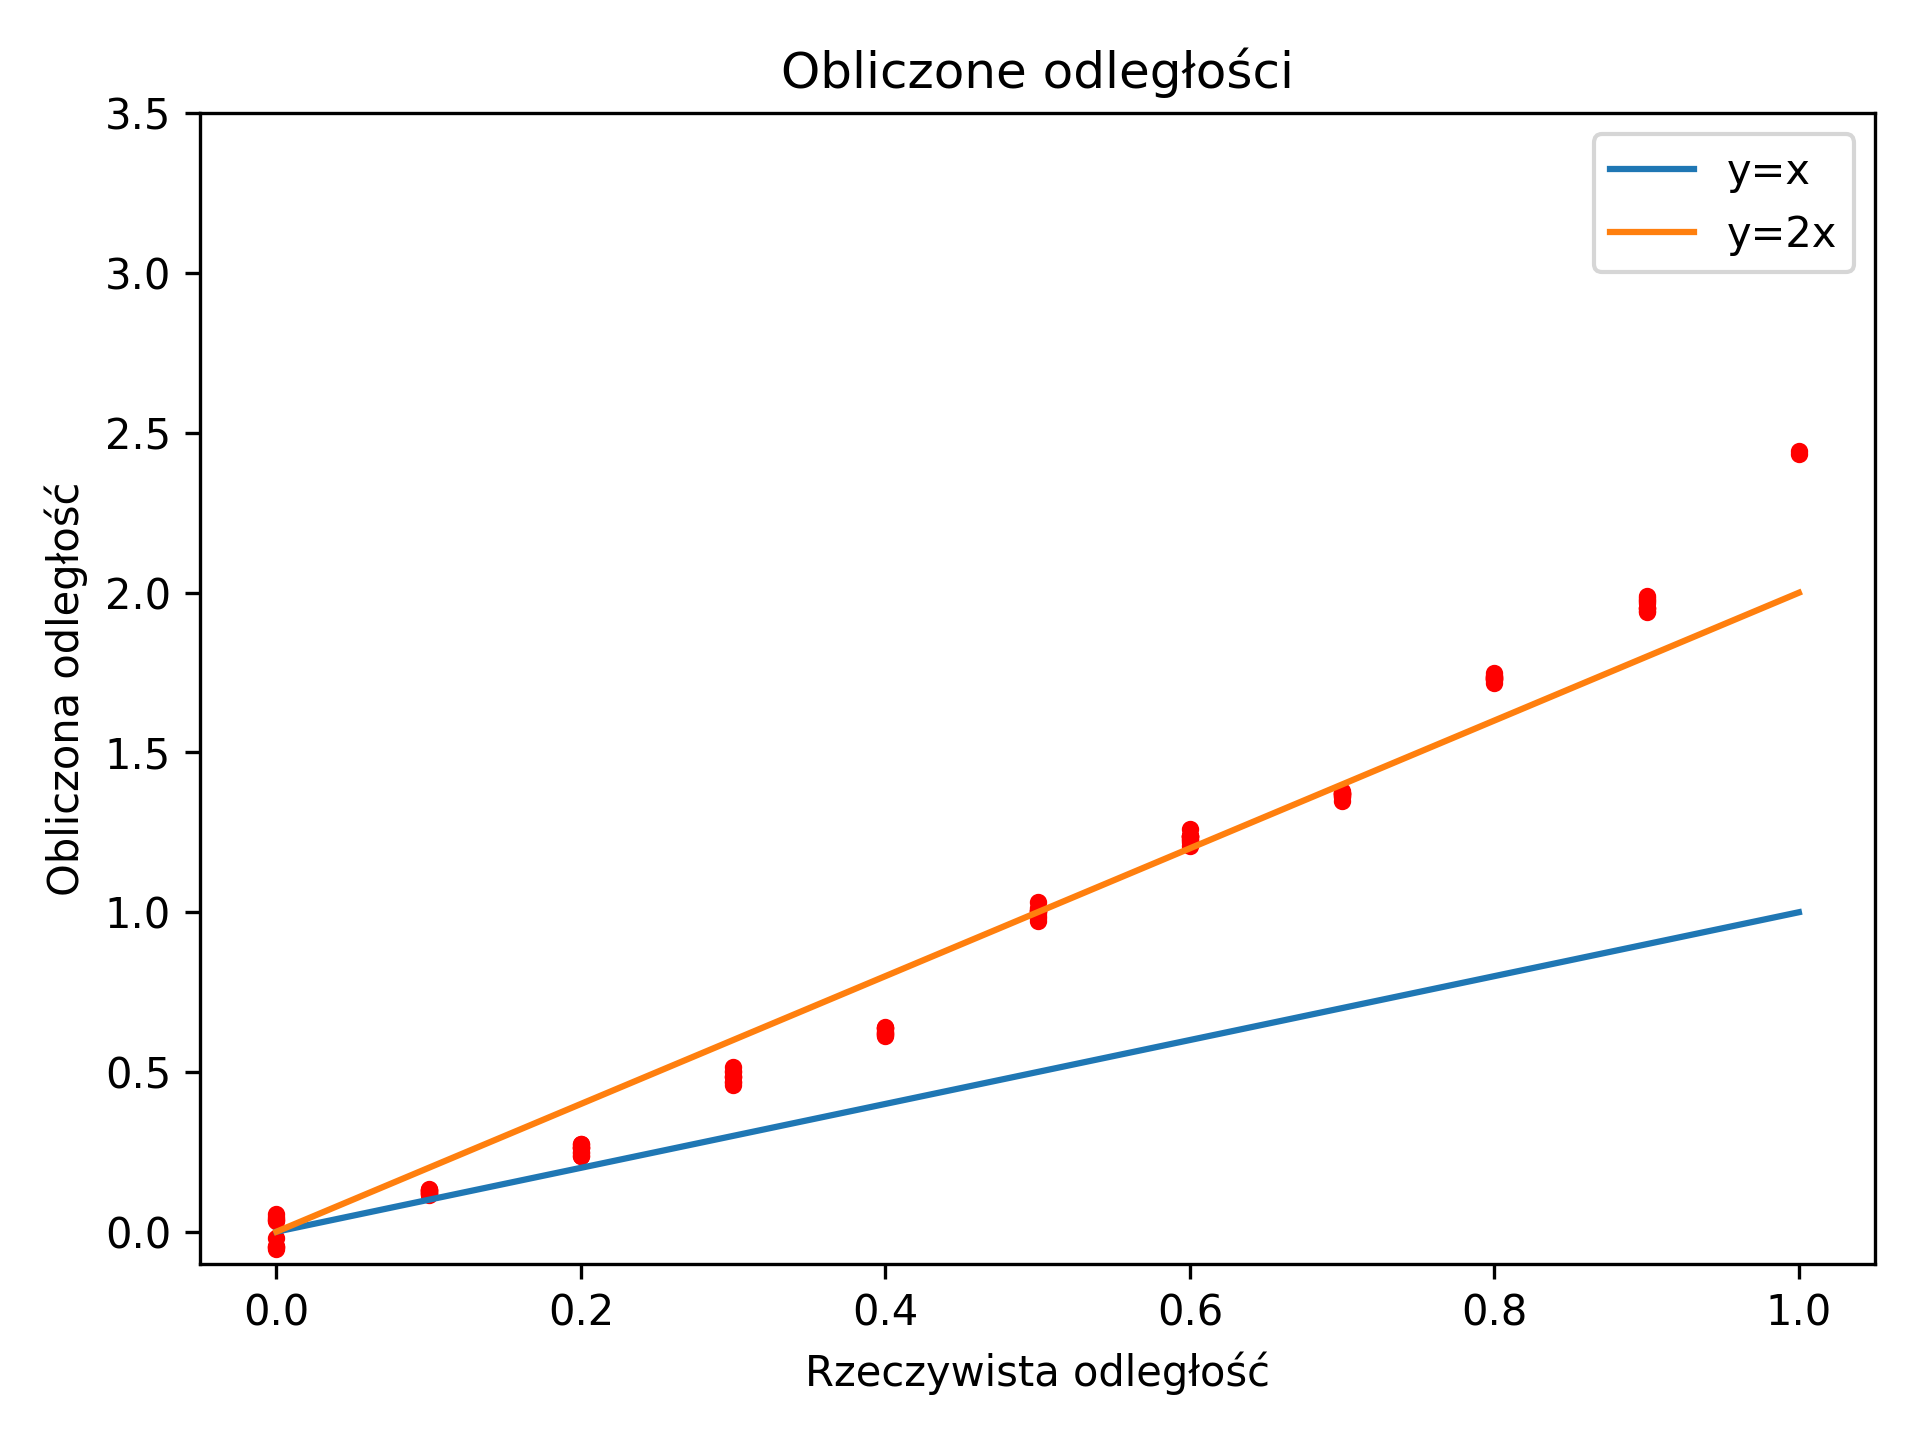
\includegraphics[width=0.49\textwidth]{pics/time_deltas_dist/dists_close.png}
        \caption{synchronizacja pomiaru przesunięć~\ref{sec:time_deltas_sync}}
        \label{pic:time_deltas_dist}
    \end{subfigure}
\end{figure}
\begin{figure}[H]
    \ContinuedFloat\centering
    \begin{subfigure}{\textwidth}
        \centering
        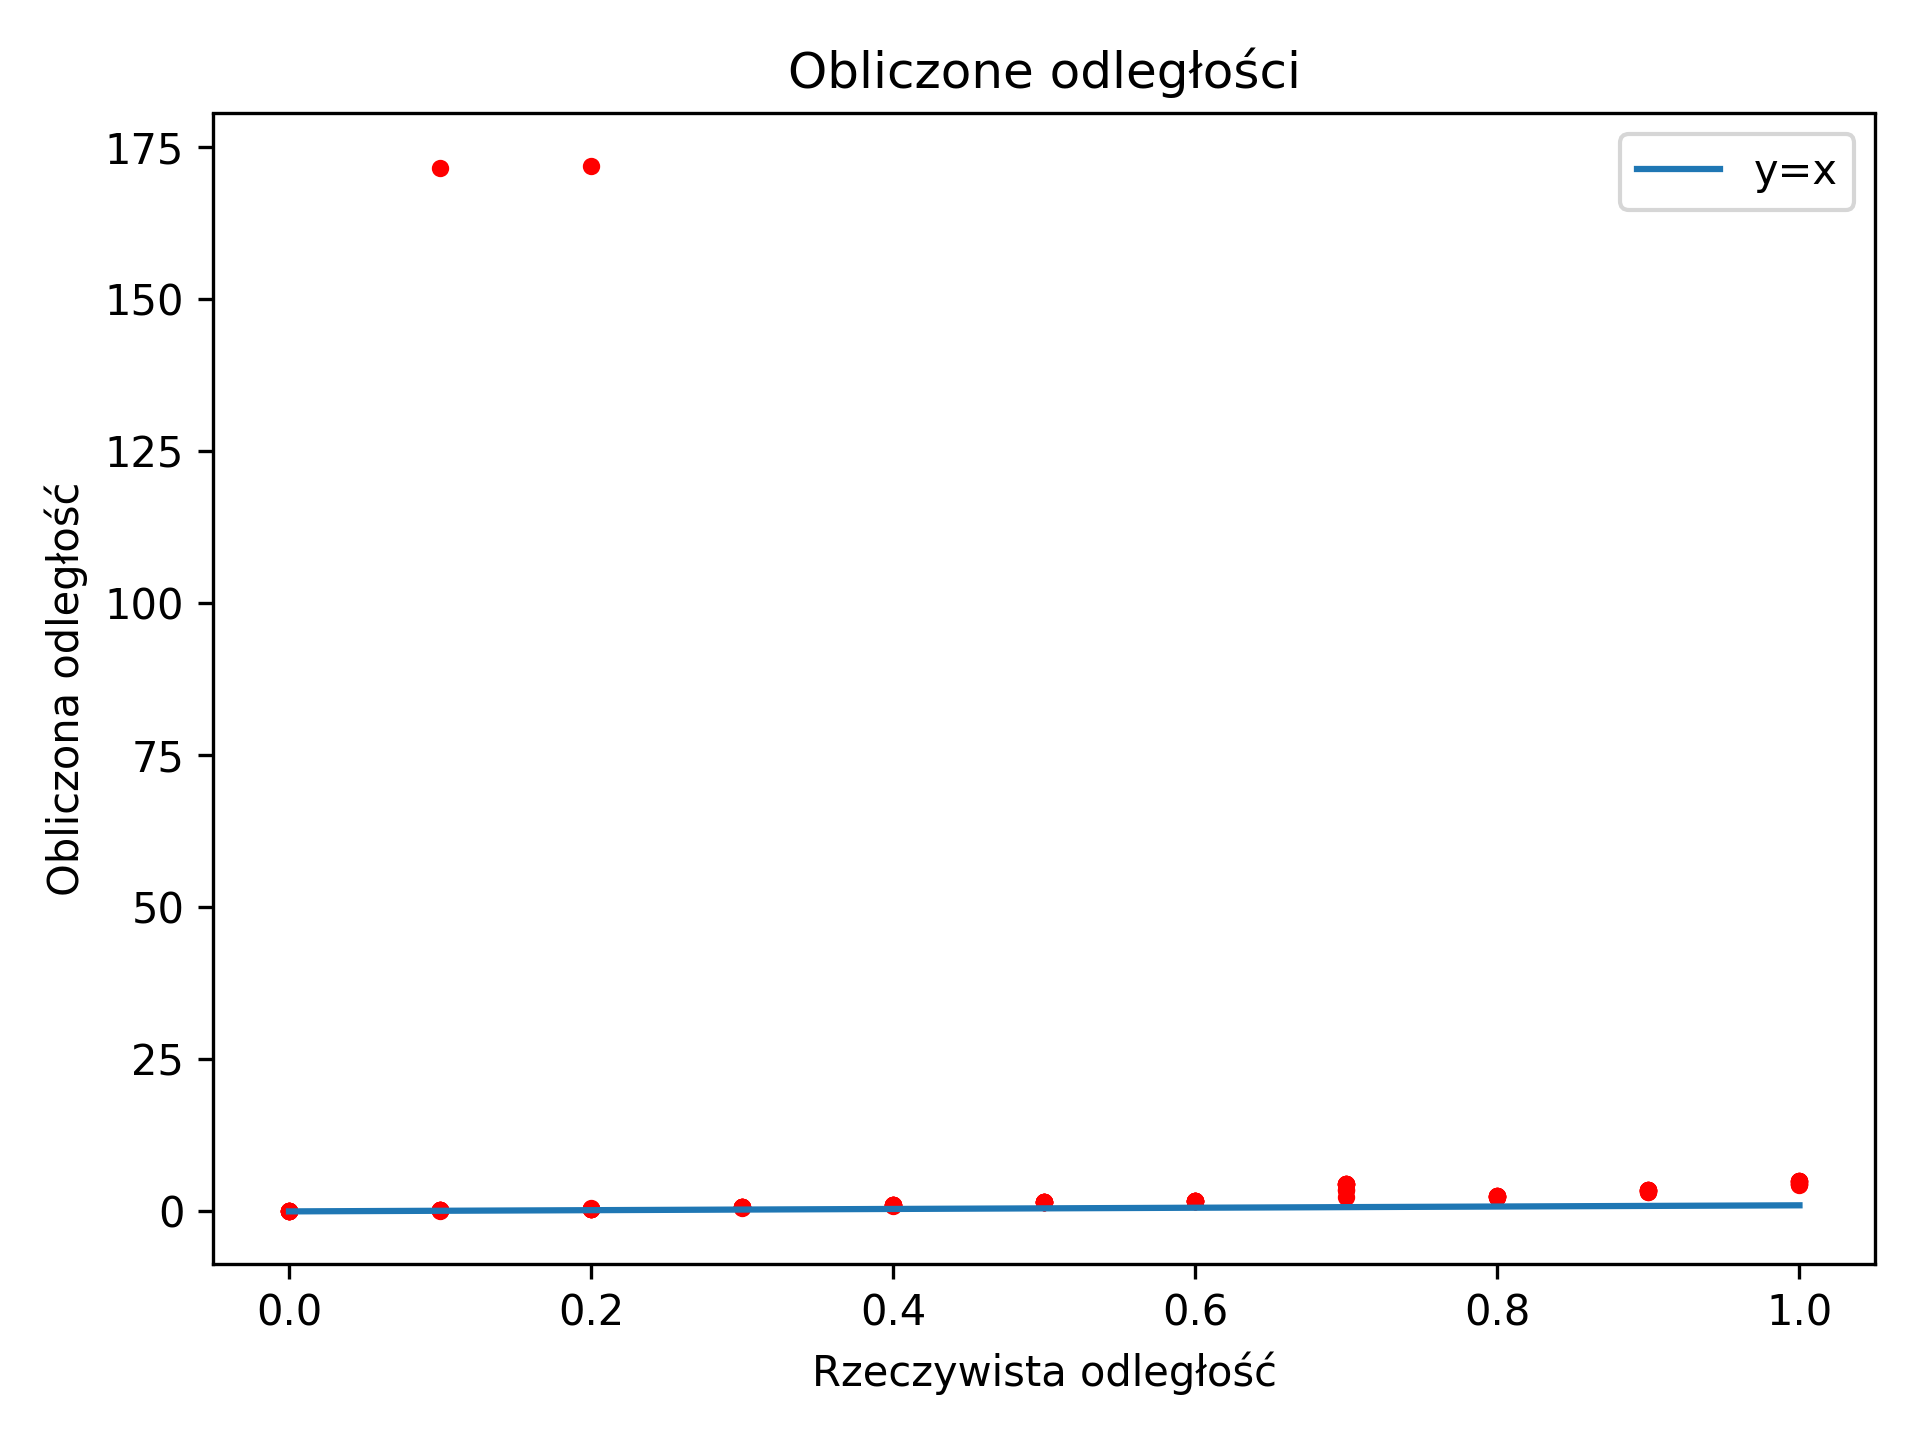
\includegraphics[width=0.49\textwidth]{pics/mic_sync_dist/dists.png}
        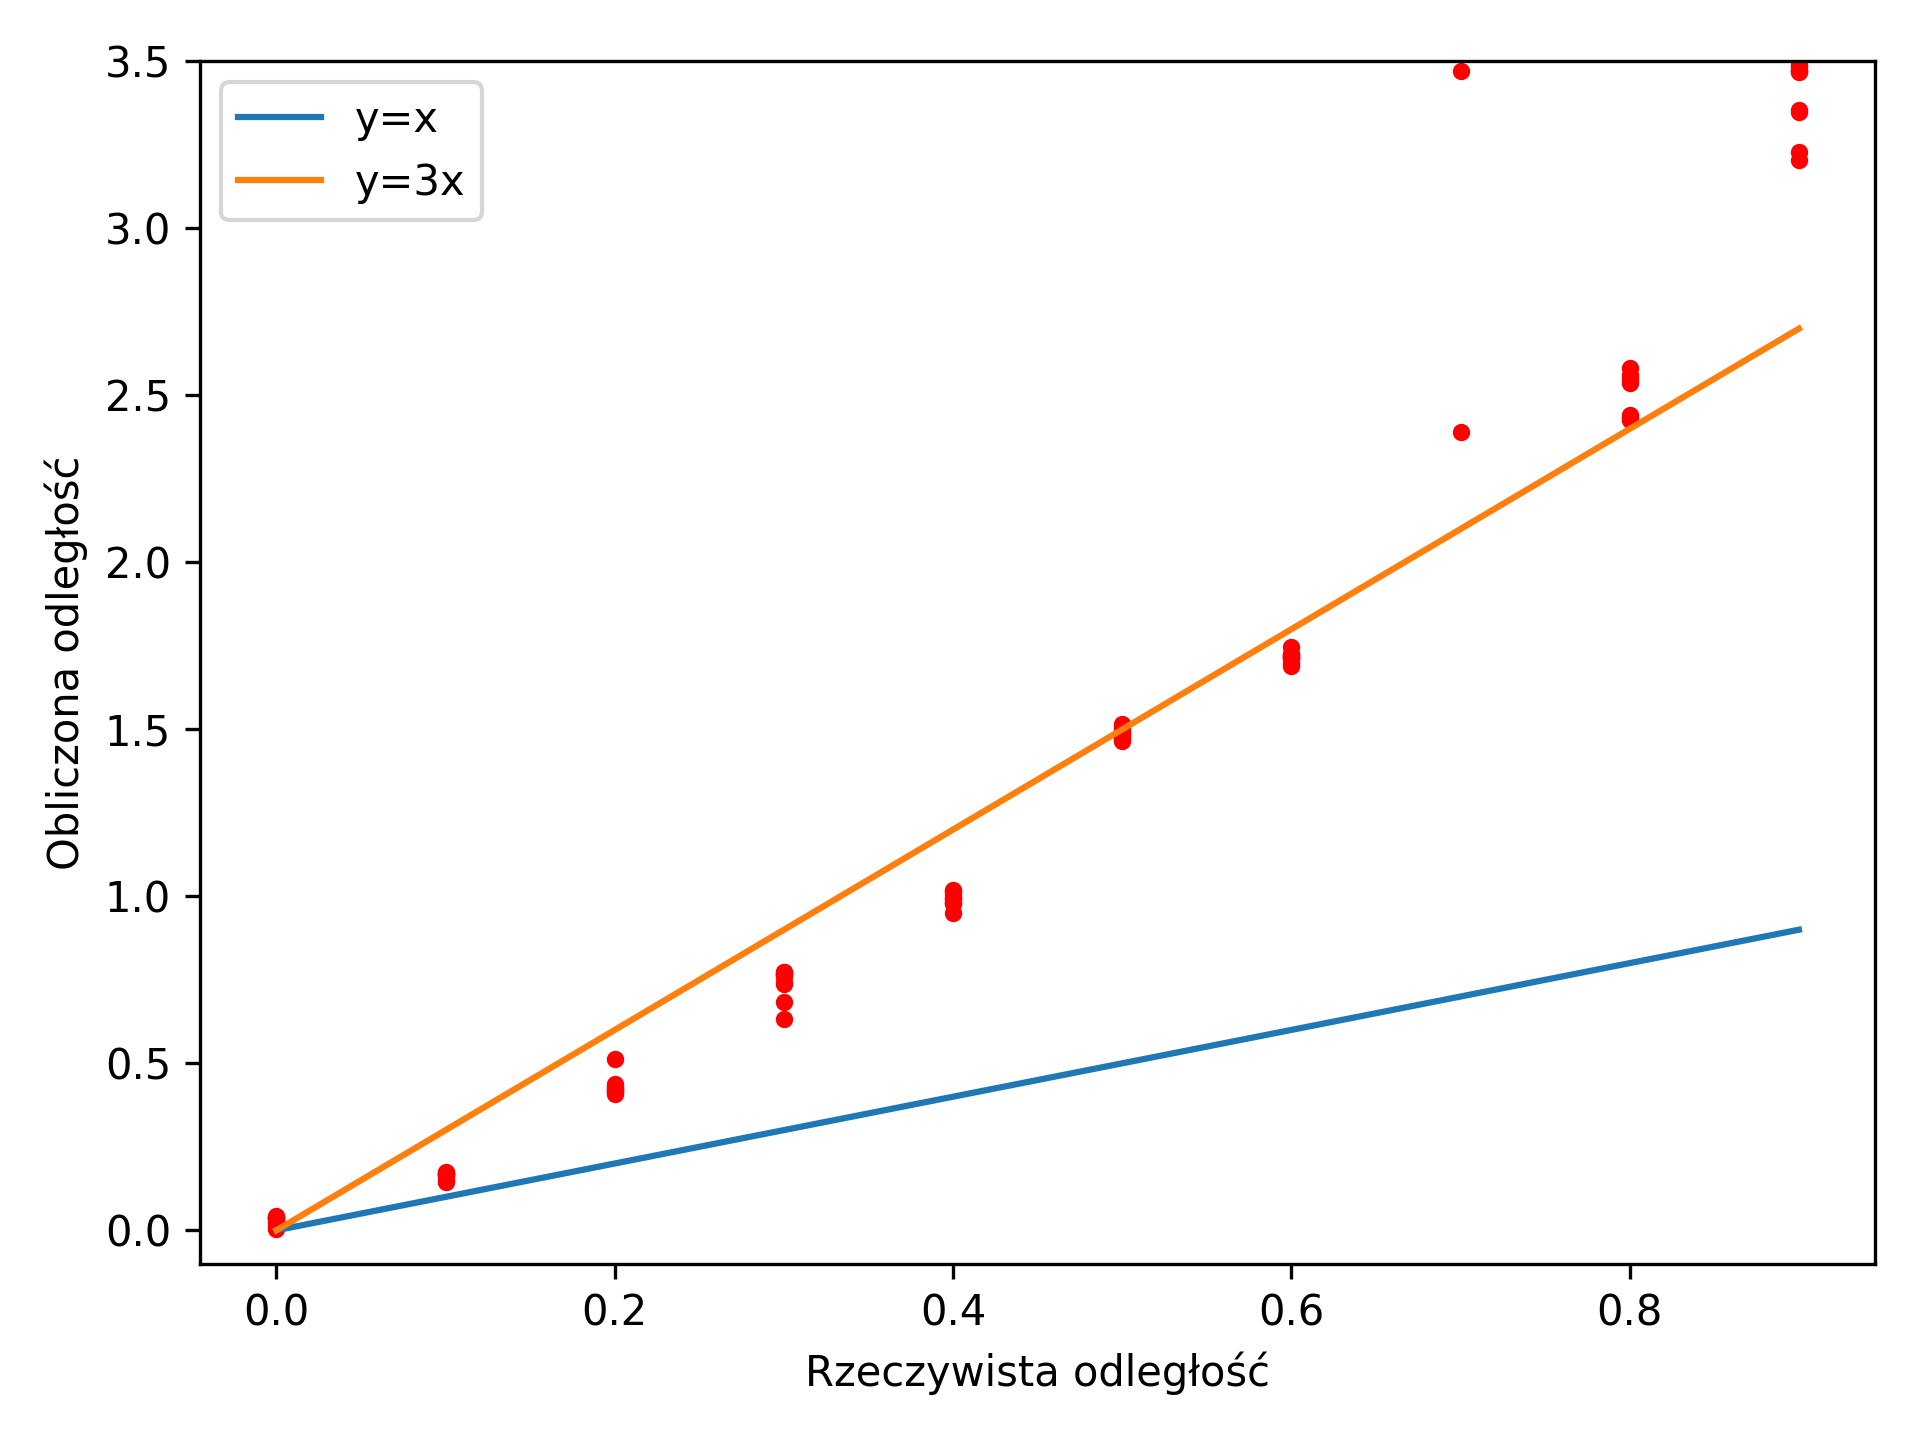
\includegraphics[width=0.49\textwidth]{pics/mic_sync_dist/dists_close.png}
        \caption{synchronizacja mikrofonowa~\ref{sec:mic_sync}}
        \label{pic:mic_sync_dist}
    \end{subfigure}
    \caption{Wyniki pomiarów odległości z użyciem rozpatrywanych synchronizacji}
    \label{fig:sync_test}
\end{figure}

Na wykresach widać, że wszystkie trzy algorytmy synchronizacji po normalizacji dają wyniki o podobnej dokładności adekwatnej do użycia w danych wejściowych multilateracji. Ciekawą jest natomiast obserwacja skalowania obliczonych odległości. Widzimy, że w przypadku~\ref{pic:ntp_sync_dist} oraz~\ref{pic:mic_sync_dist} otrzymane wartości leżą blisko trzykrotności rzeczywistej badanej odległości, natomiast w~\ref{pic:time_deltas_dist} blisko dwukrotności. W kolejnym rozdziale pochylimy się nad możliwymi przyczynami i rozwiązaniem tego zachowania.
\chapter{Multilateriacja}\label{chap:multilateration}

\section{Przygotowanie danych wejściowych}

Aby otrzymać poprawne wyniki algorytmu multilateracji dane wejściowe, w naszym przypadku odległości między węzłami odbiorczymi a nadajnikiem powinny być jak najbliższe rzeczywistym odległościom z możliwie małymi odchyleniami. Będziemy kontynuować usprawnianie metod uzyskiwania poprawnych wyników zapoczątkowane w rozdziale poprzednim.

\subsection{Korekcja odległości}

W wynikach eksperymentów porównawczych metod synchronizacji czasu węzłów przeprowadzonych w rozdziale~\ref{chap:time_sync}.\ zaobserwowaliśmy skalowanie wyników na pierwszy rzut oka zachowujące się liniowo. Przyjrzyjmy się teraz dokładnie temu zjawisku. W tym i kolejnych przypadkach będziemy używać już jedynie synchronizacji sprzętowej z użyciem mikrofonów ze względu na brak konieczności dodatkowej kalibracji przesunięcia punktu 0.

Prawdopodobnym powodem skalowania obliczanych odległości może być odczyt zmiany sygnału mikrofonowego odczytywanego przez mikrokontroler. Poniższe wykresy są wynikiem czterech kolejnych eksperymentów, w których jedyną zmienną była czułość zintegrowanego wzmacniacza mikrofonu. Wzmacniacz ten nie pozwala na precyzyjną regulację, a jedynie na zmianę rezystancji wbudowanego potencjometru. Ponieważ przedział czułości odpowiadający wykrywaniu sygnału węzła nadającego przy jednoczesnym zminimalizowaniu fałszywych aktywacji jest niewielki (około $\frac{1}{8}$ obrotu potencjometru) cztery zbadane przypadki nie dzielą równo badanego zakresu. Rozpoczynając od największej możliwej czułości przy każdym kolejnym eksperymencie zmniejszano ją póki pozwalała wciąż na wykrywanie sygnału z badanych odległości.

\begin{figure}[h]
\centering
    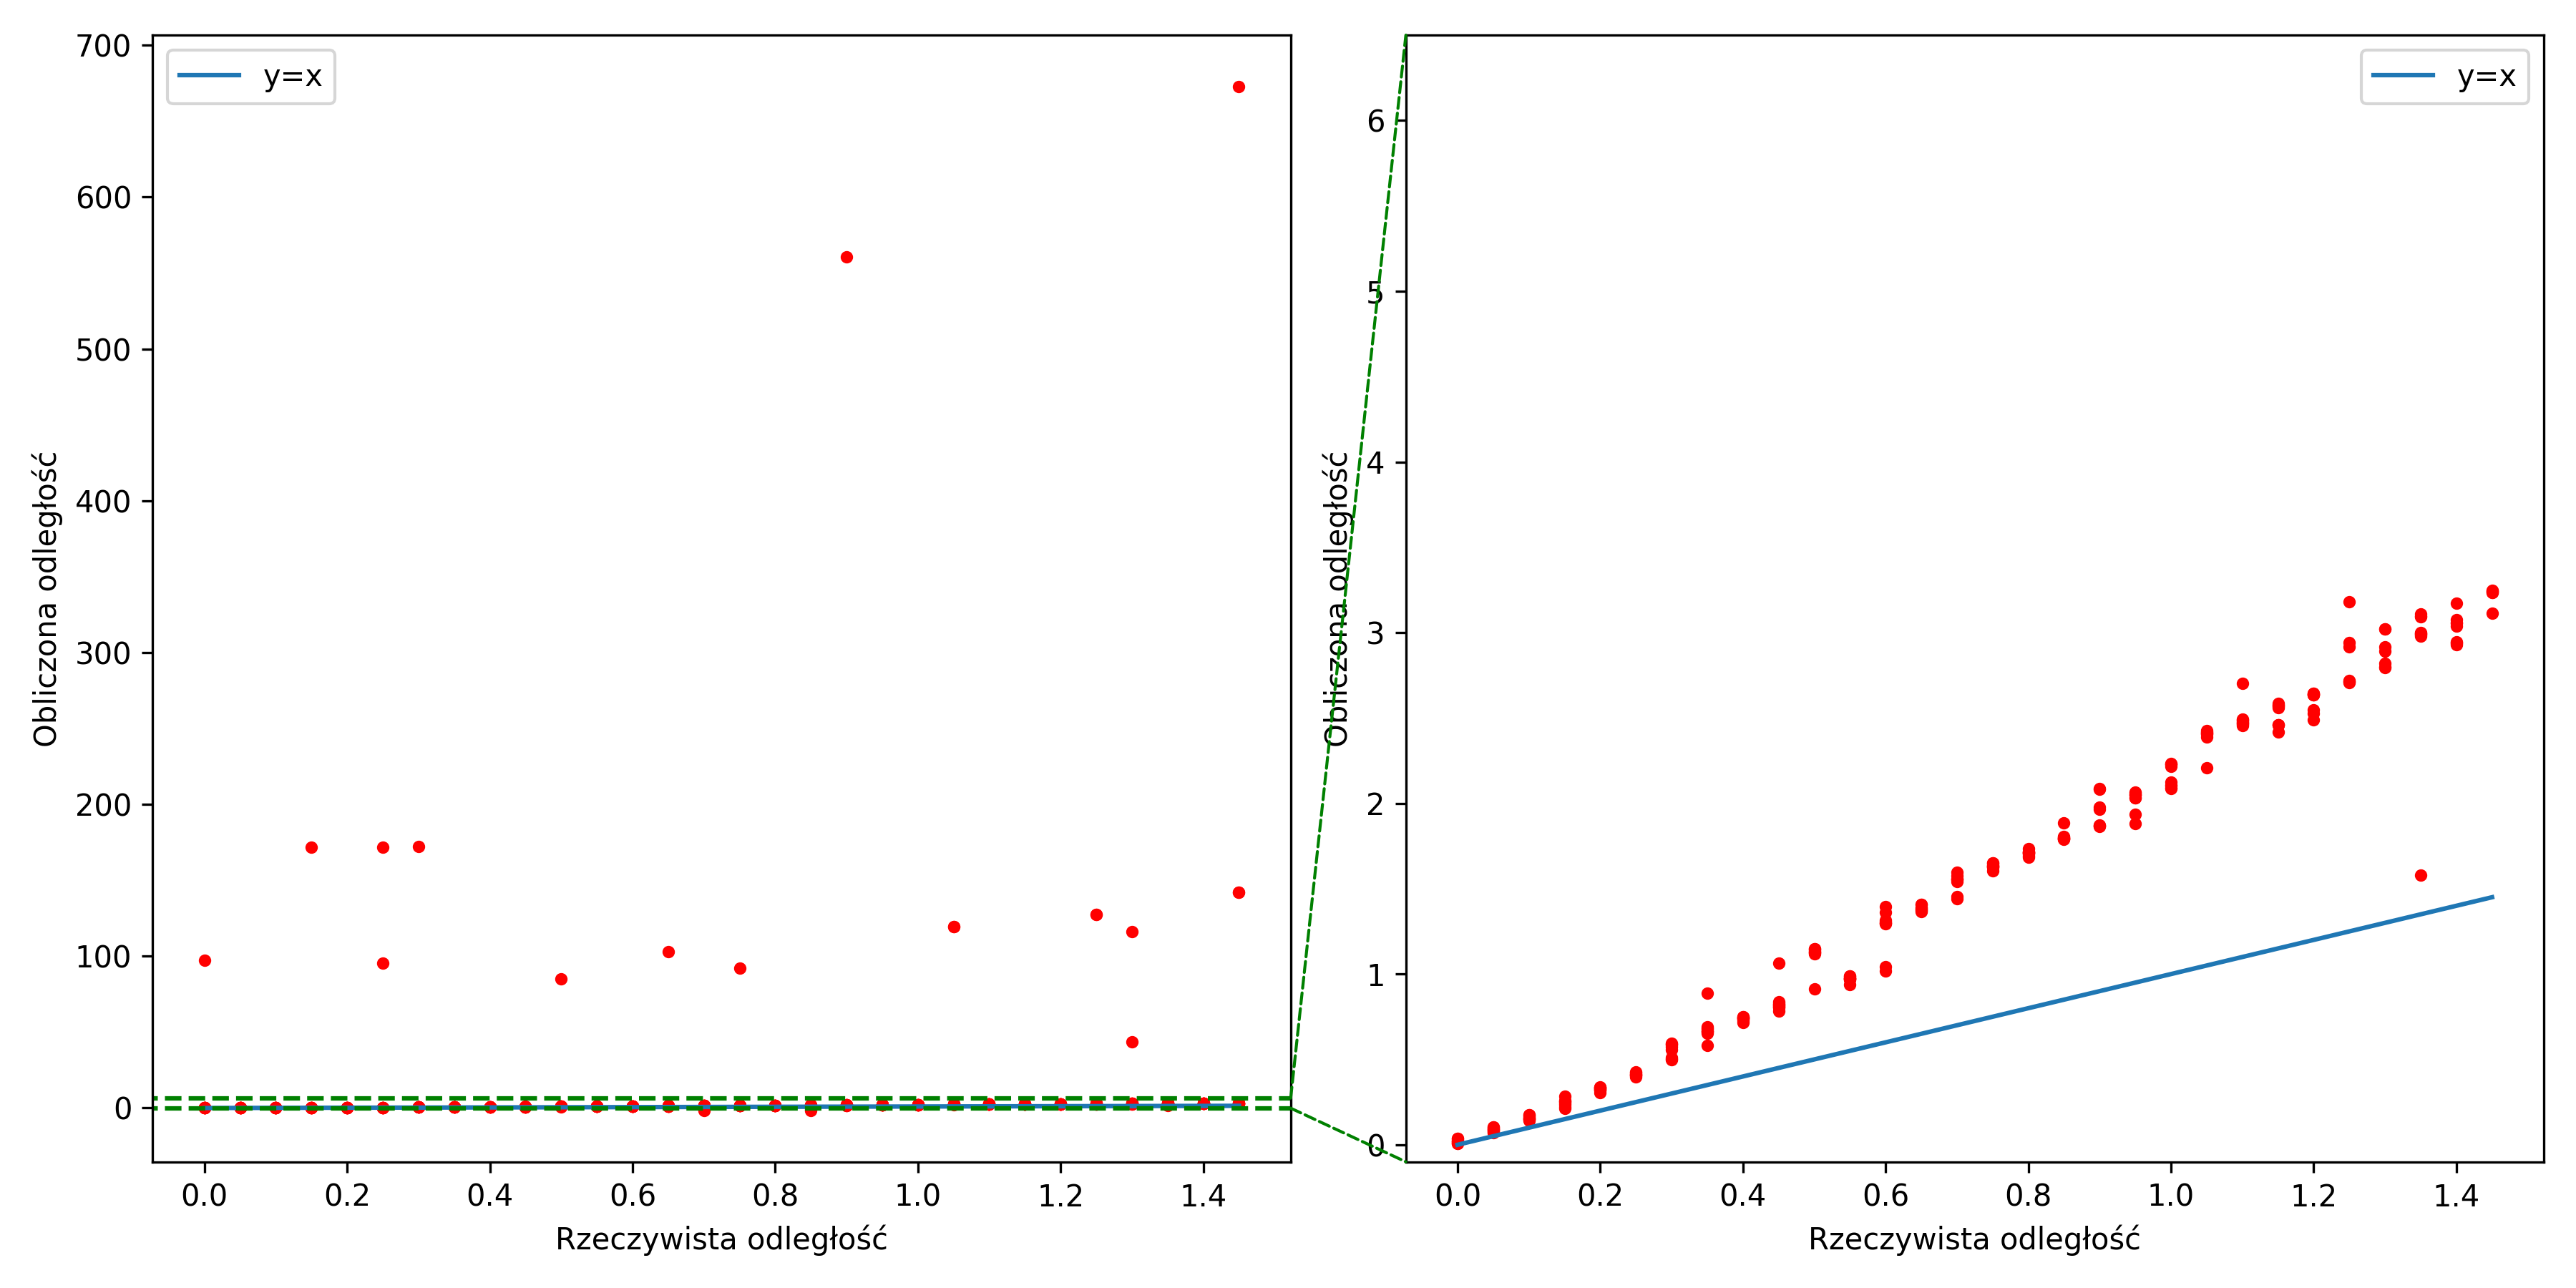
\includegraphics[width=.49\textwidth]{pics/mic_sync_dist/dists_long_0.png}
    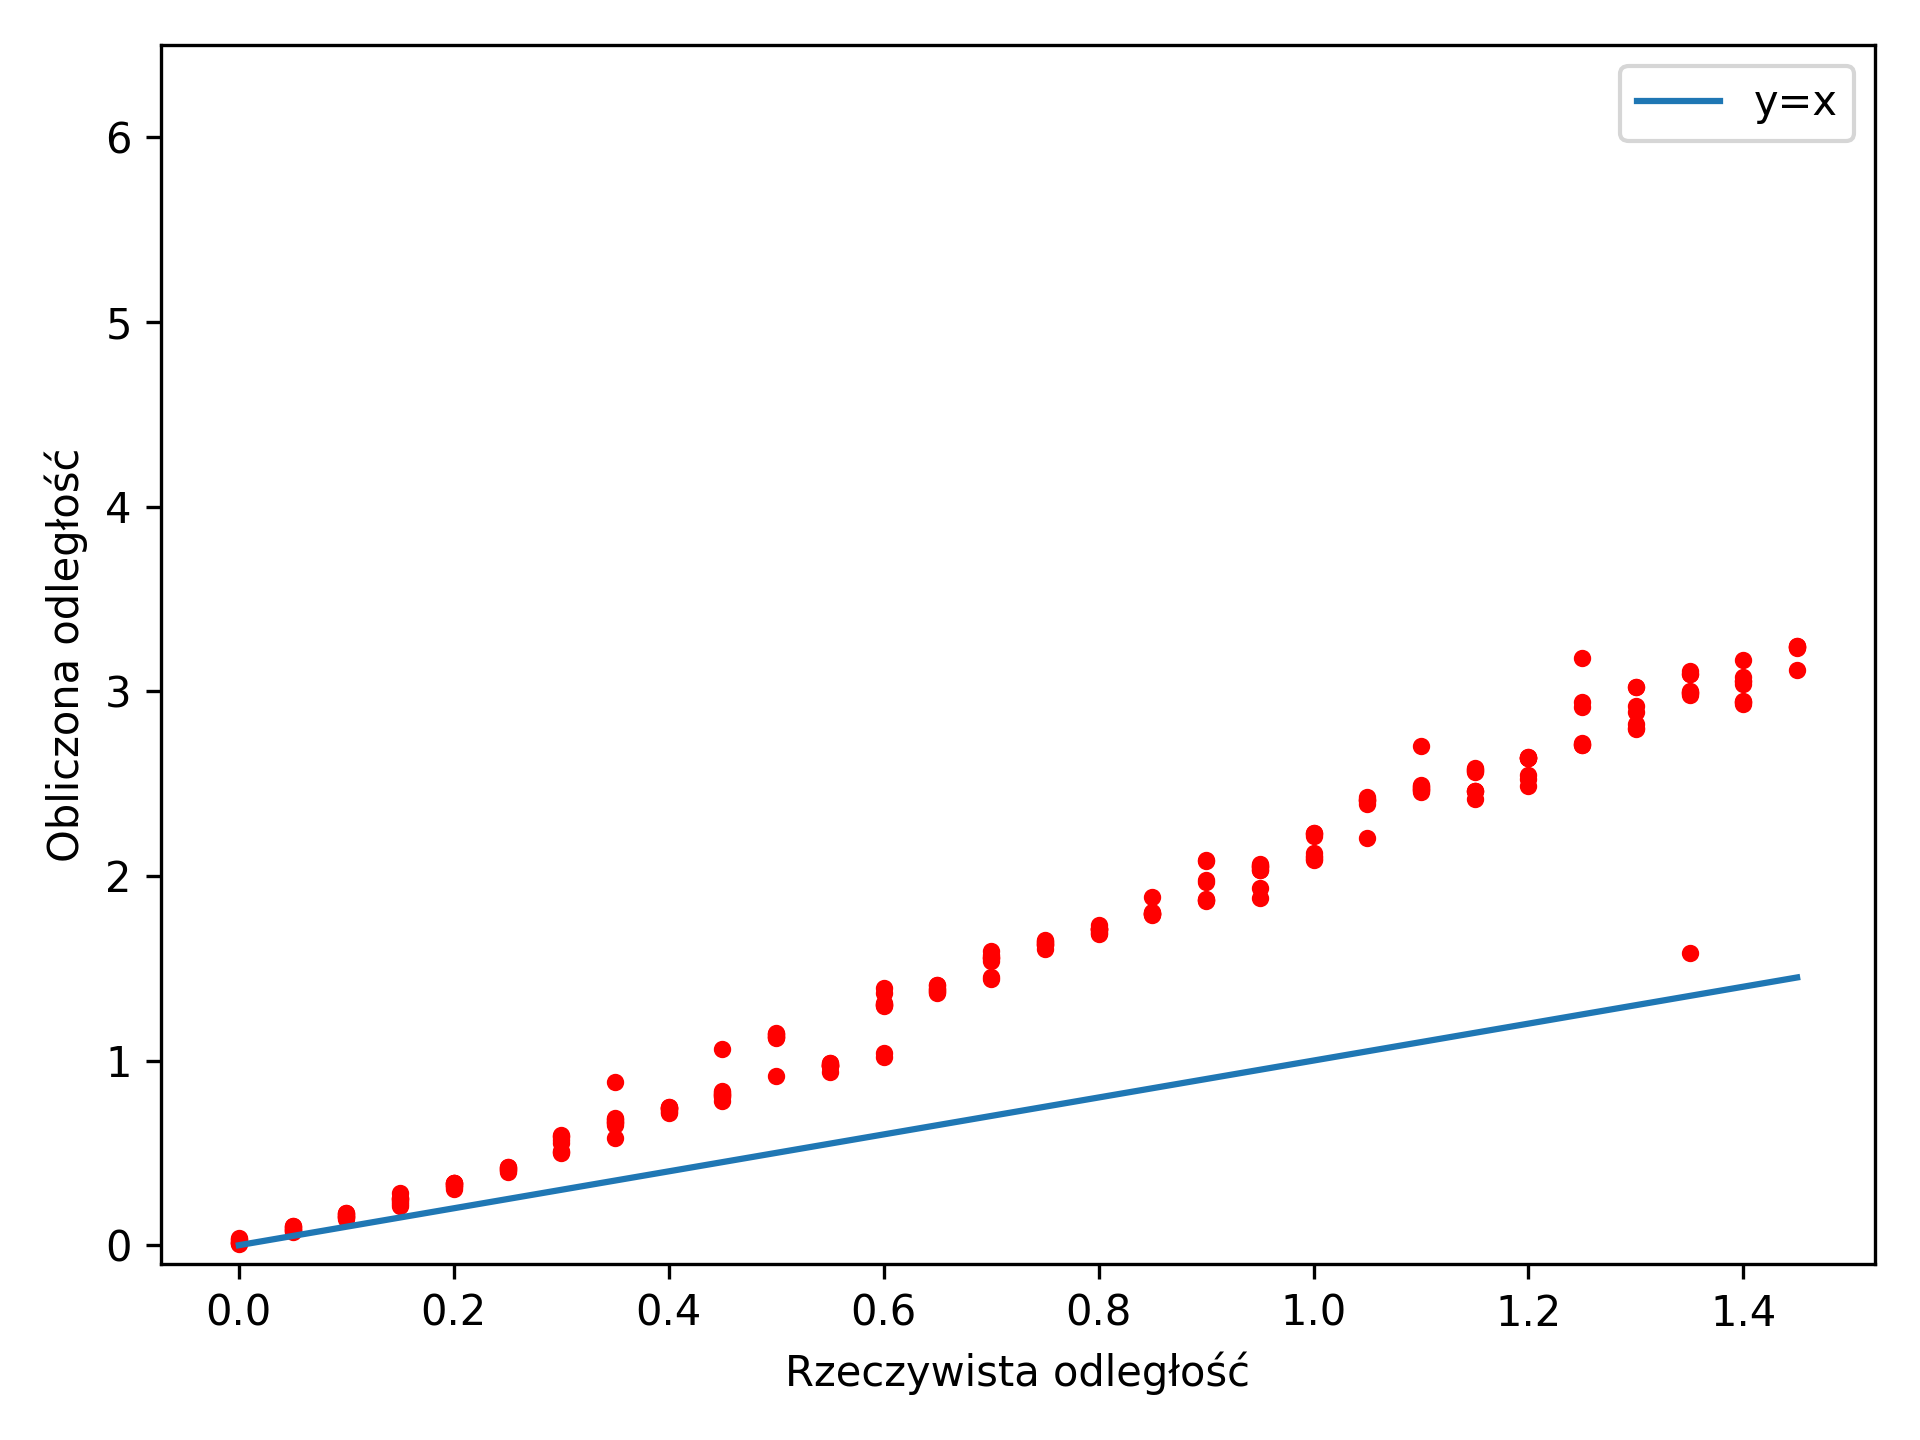
\includegraphics[width=.49\textwidth]{pics/mic_sync_dist/dists_close_long_0.png}
\caption{Pomiar obliczanych odległości 1.}
\label{pic:slope_test_0}
\end{figure}

\begin{figure}[h]
\centering
    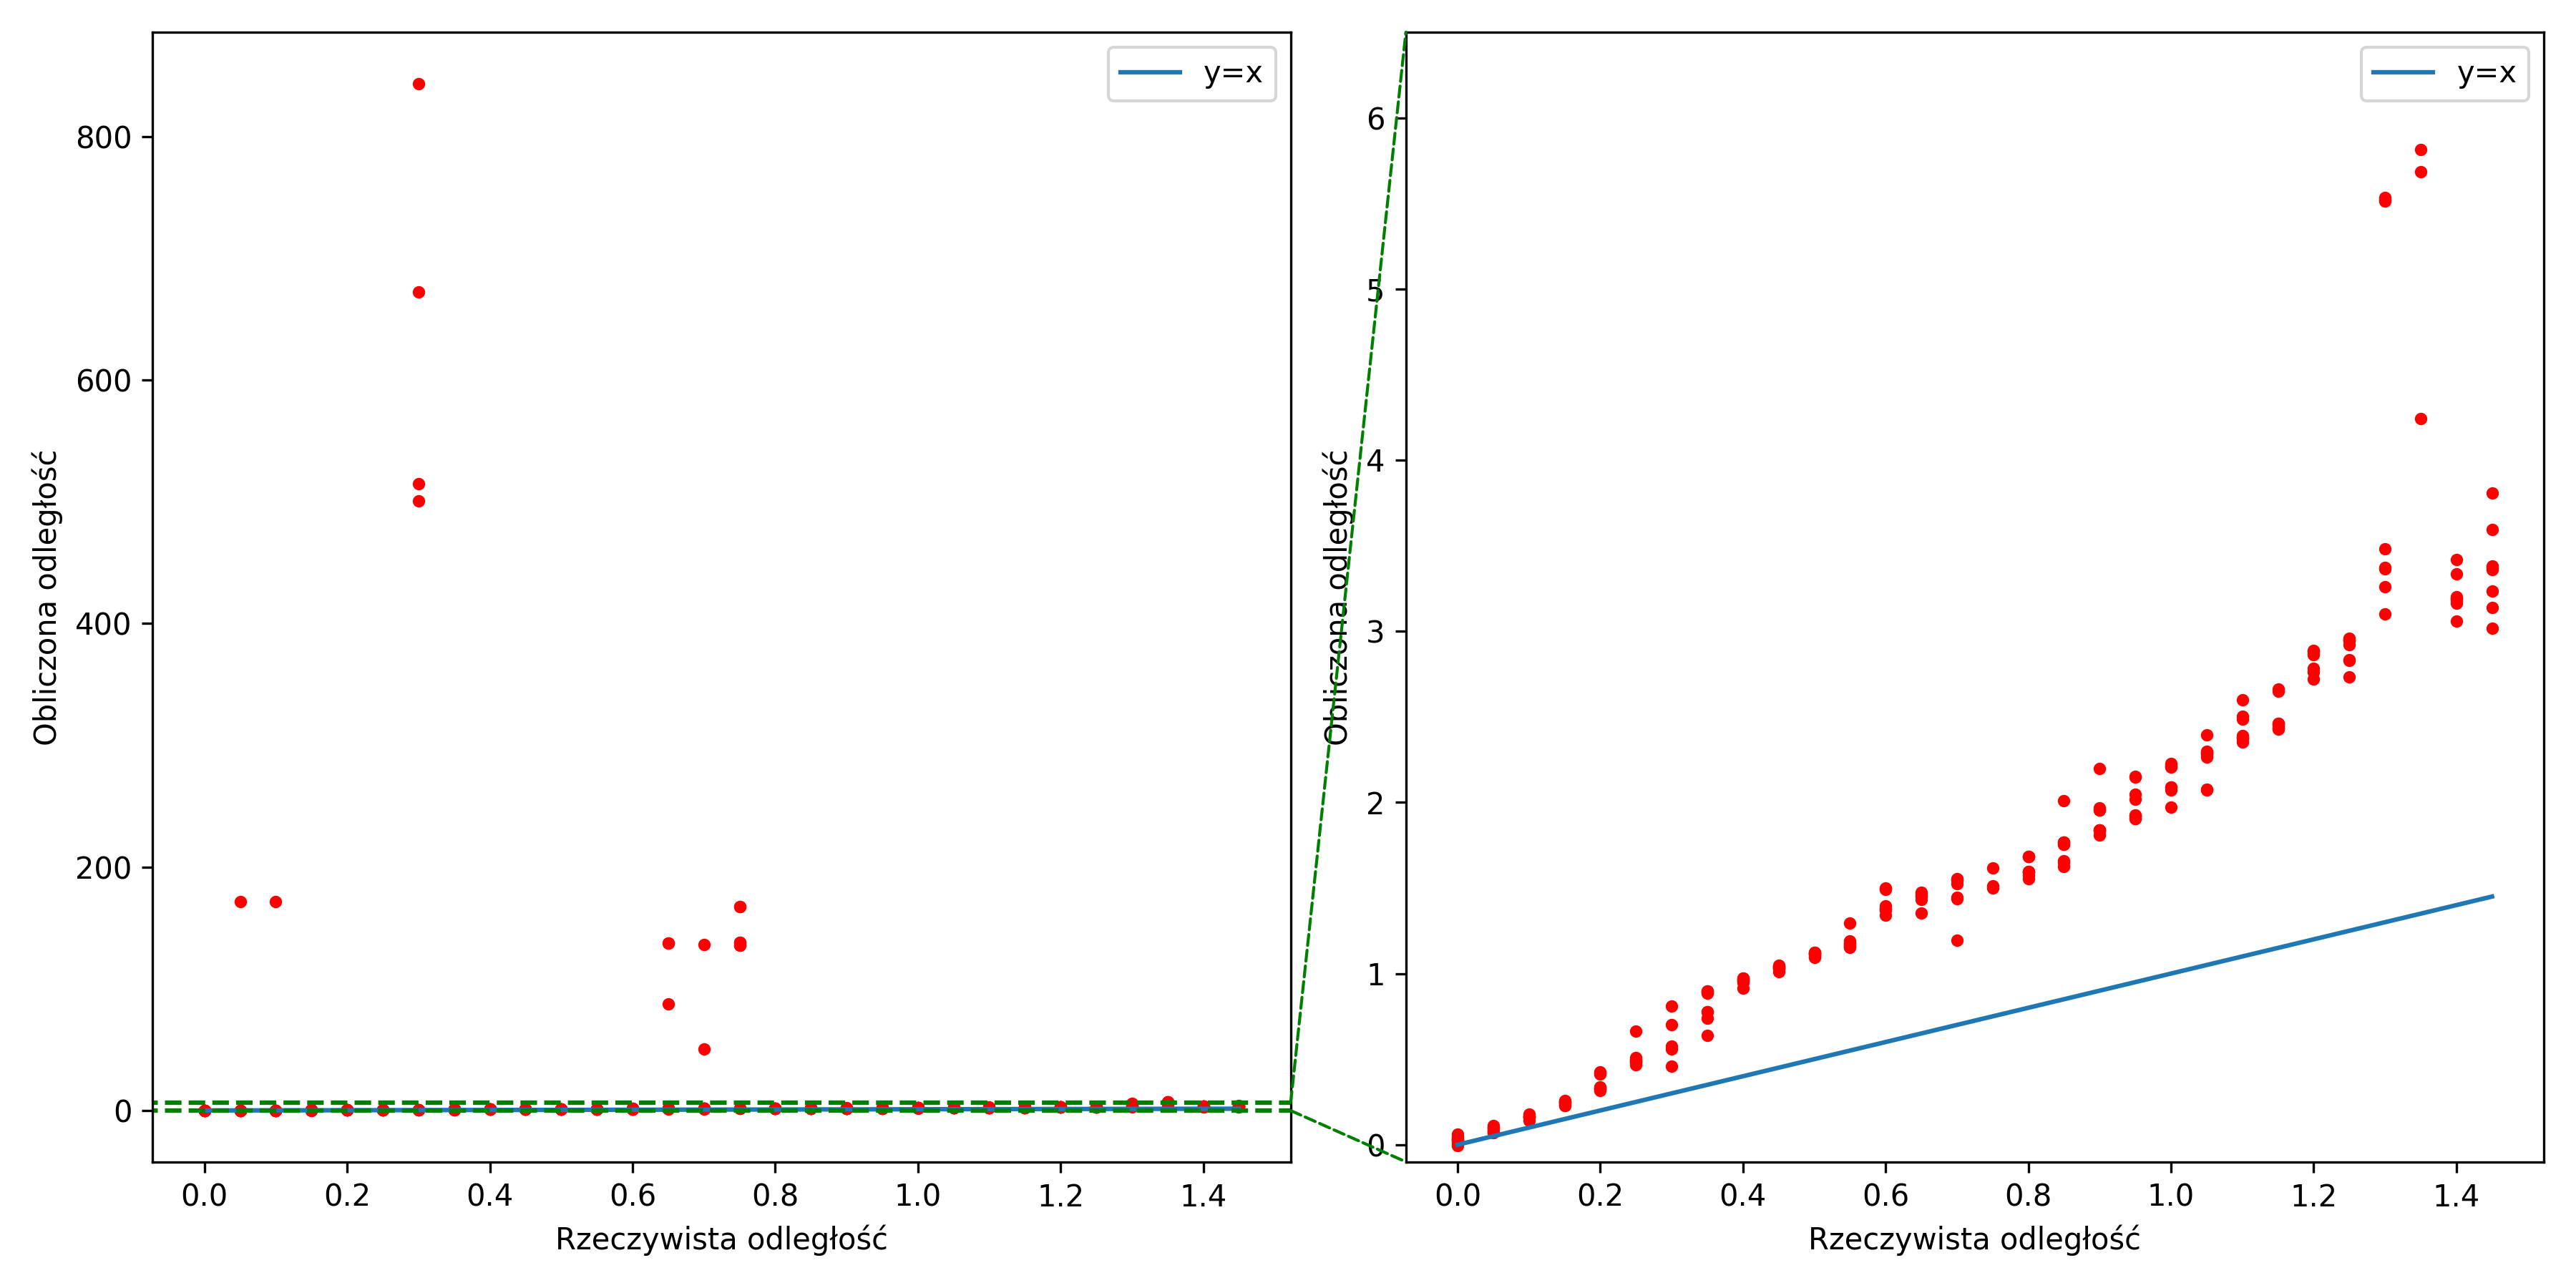
\includegraphics[width=.49\textwidth]{pics/mic_sync_dist/dists_long_1.png}
    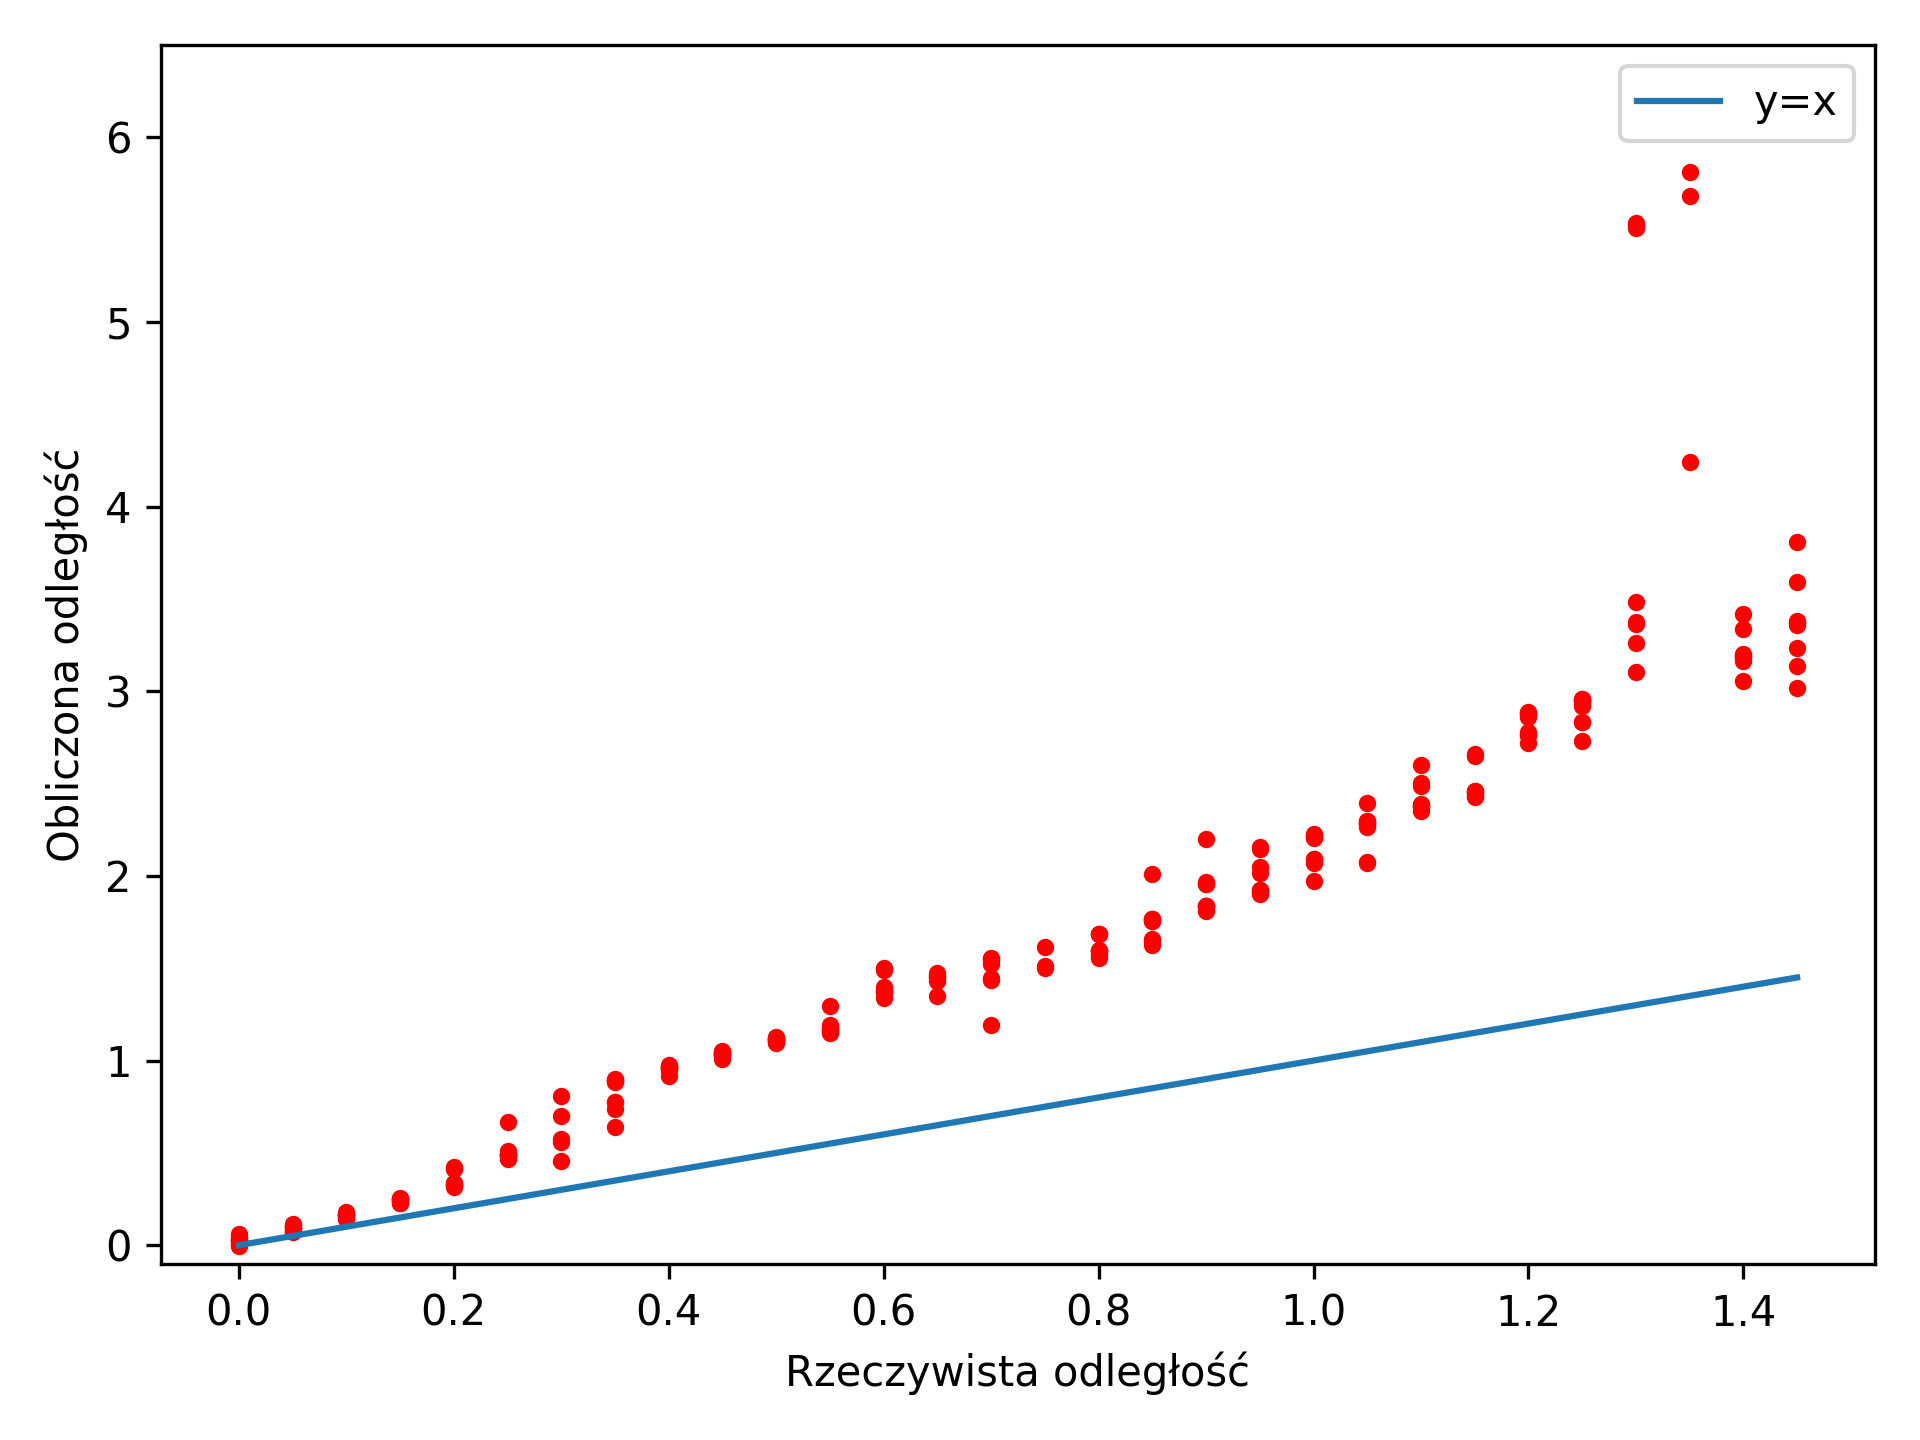
\includegraphics[width=.49\textwidth]{pics/mic_sync_dist/dists_close_long_1.png}
\caption{Pomiar obliczanych odległości 2.}
\label{pic:slope_test_1}
\end{figure}

\begin{figure}[h]
\centering
    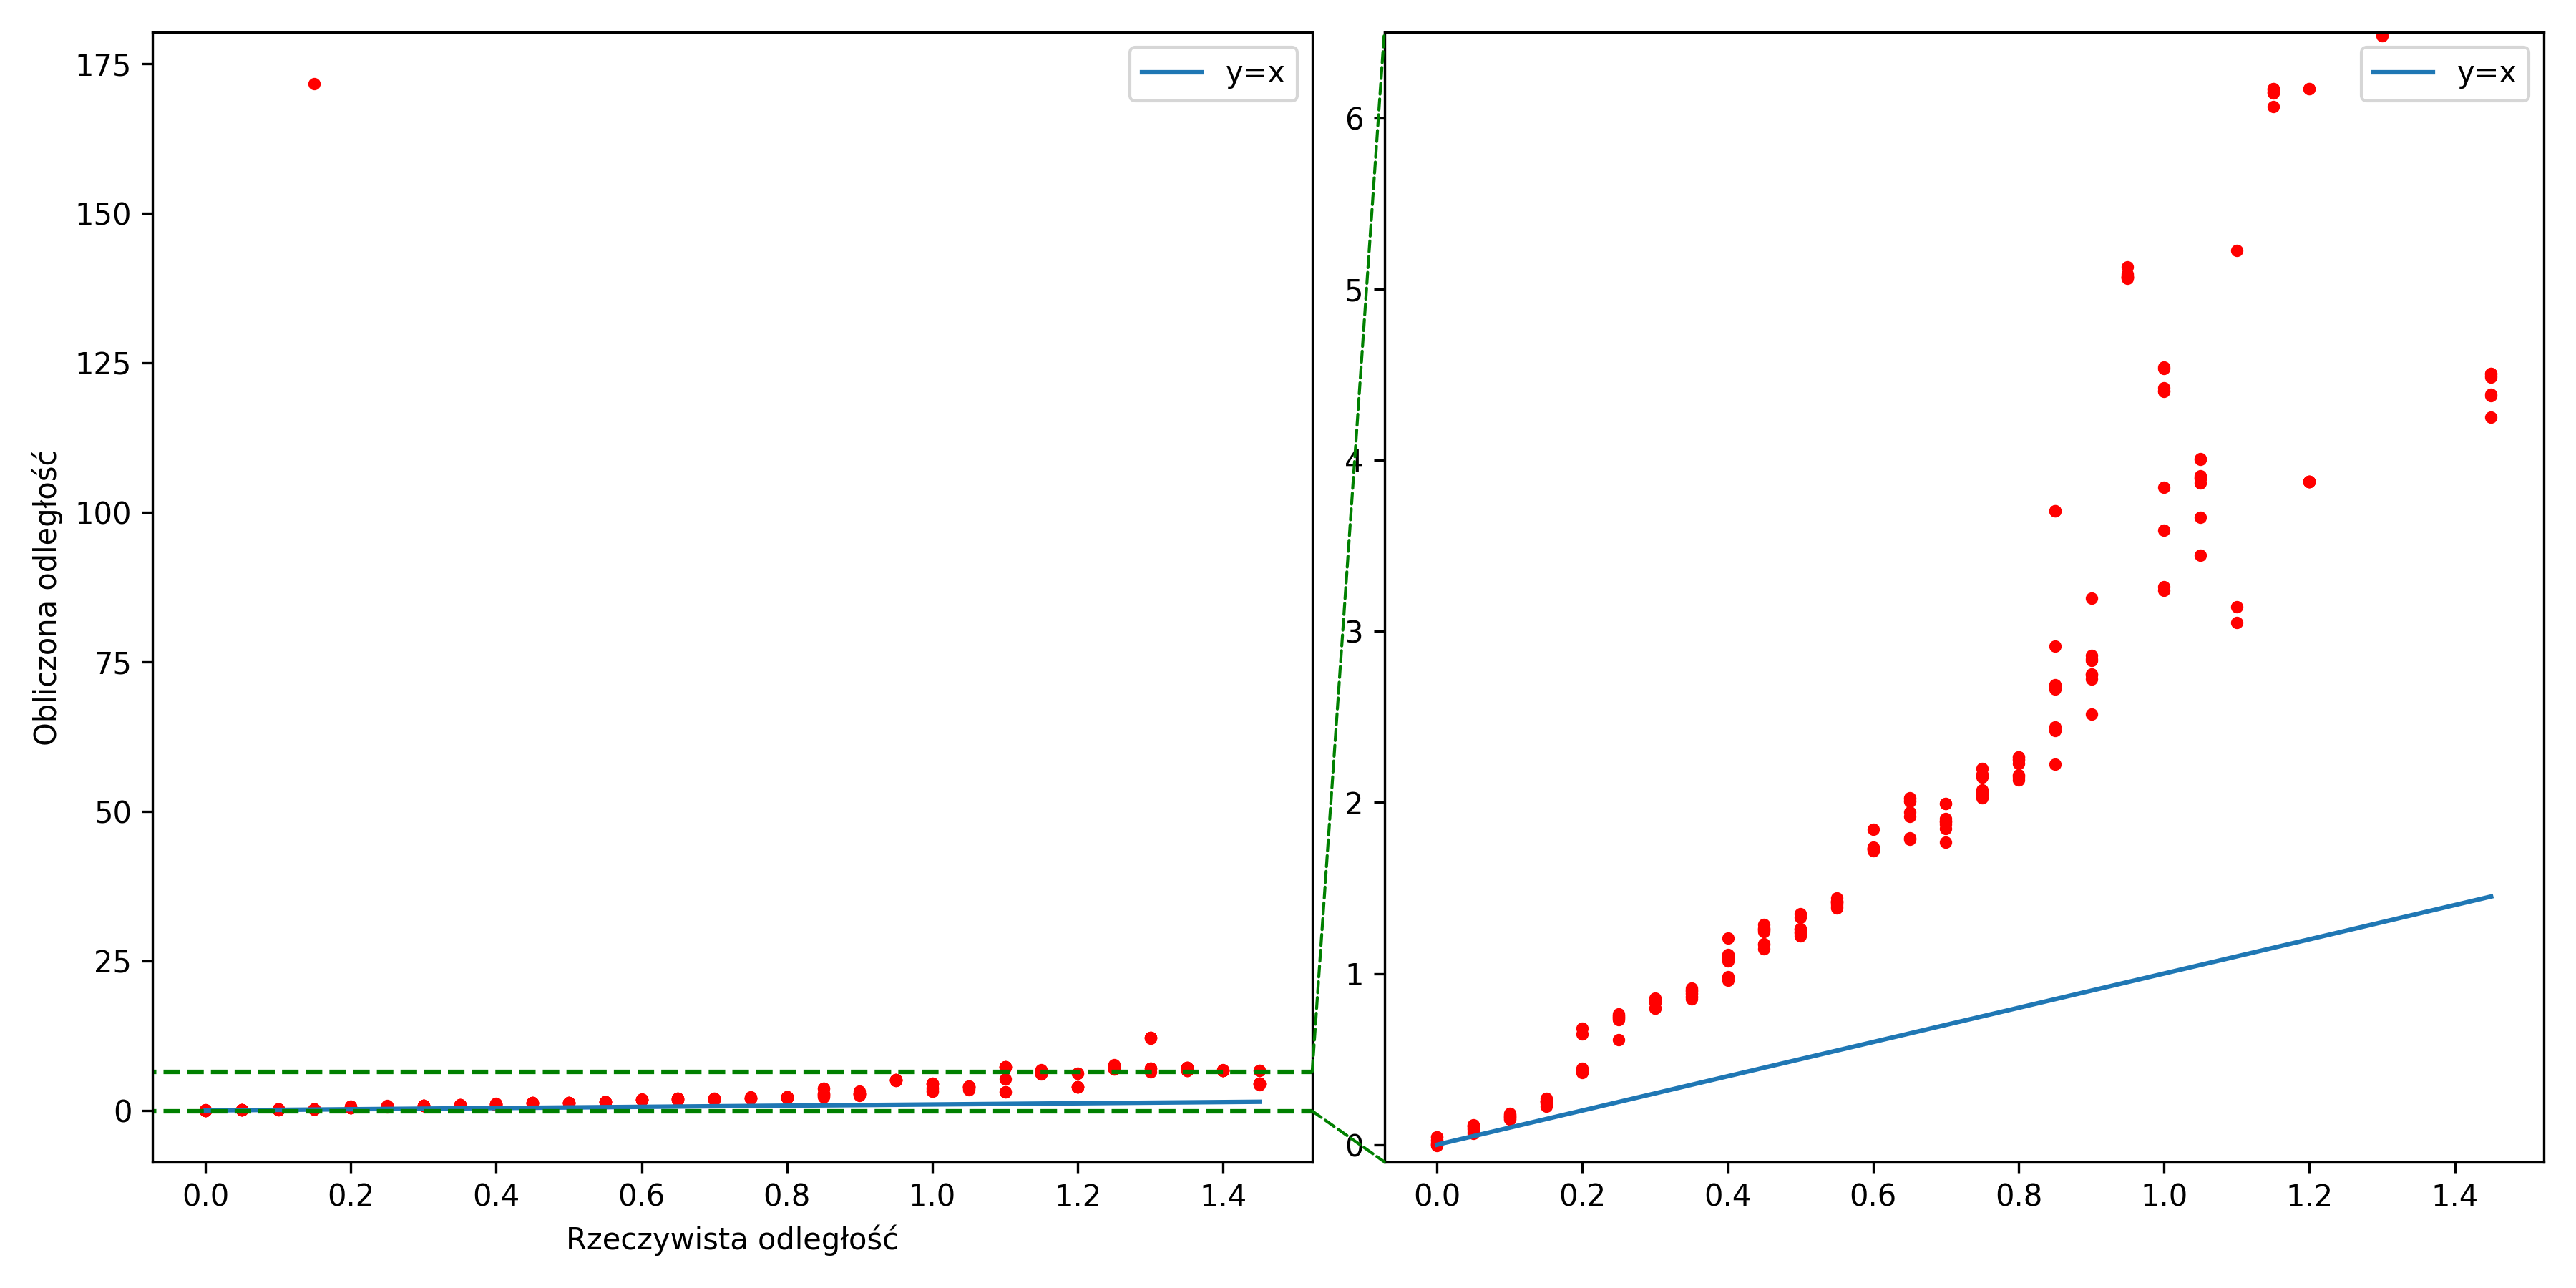
\includegraphics[width=.49\textwidth]{pics/mic_sync_dist/dists_long_2.png}
    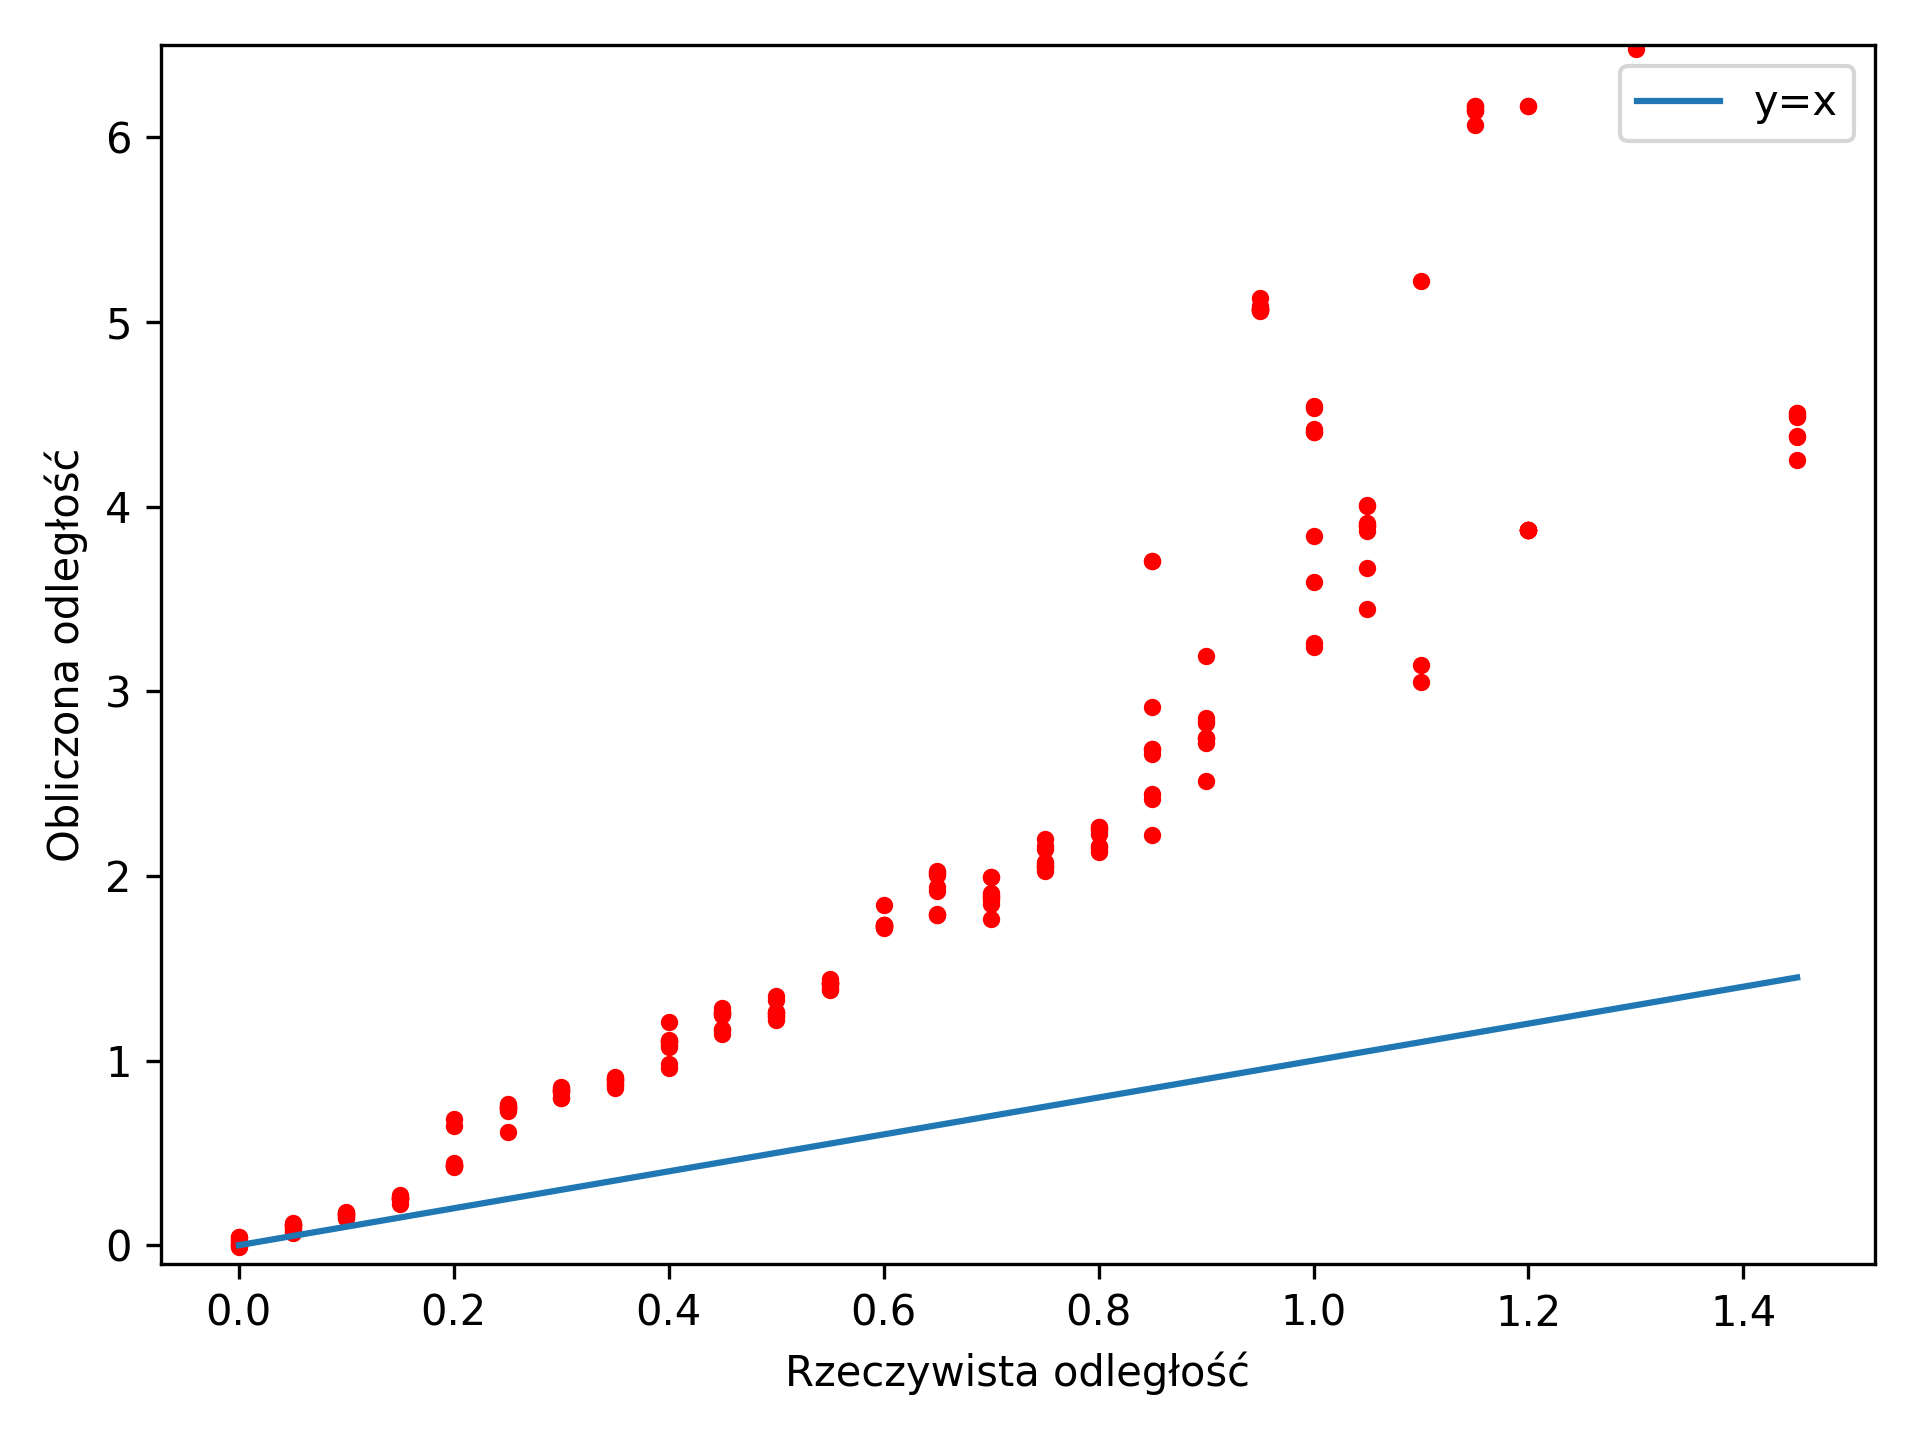
\includegraphics[width=.49\textwidth]{pics/mic_sync_dist/dists_close_long_2.png}
\caption{Pomiar obliczanych odległości 3.}
\label{pic:slope_test_2}
\end{figure}

\begin{figure}[h]
\centering
    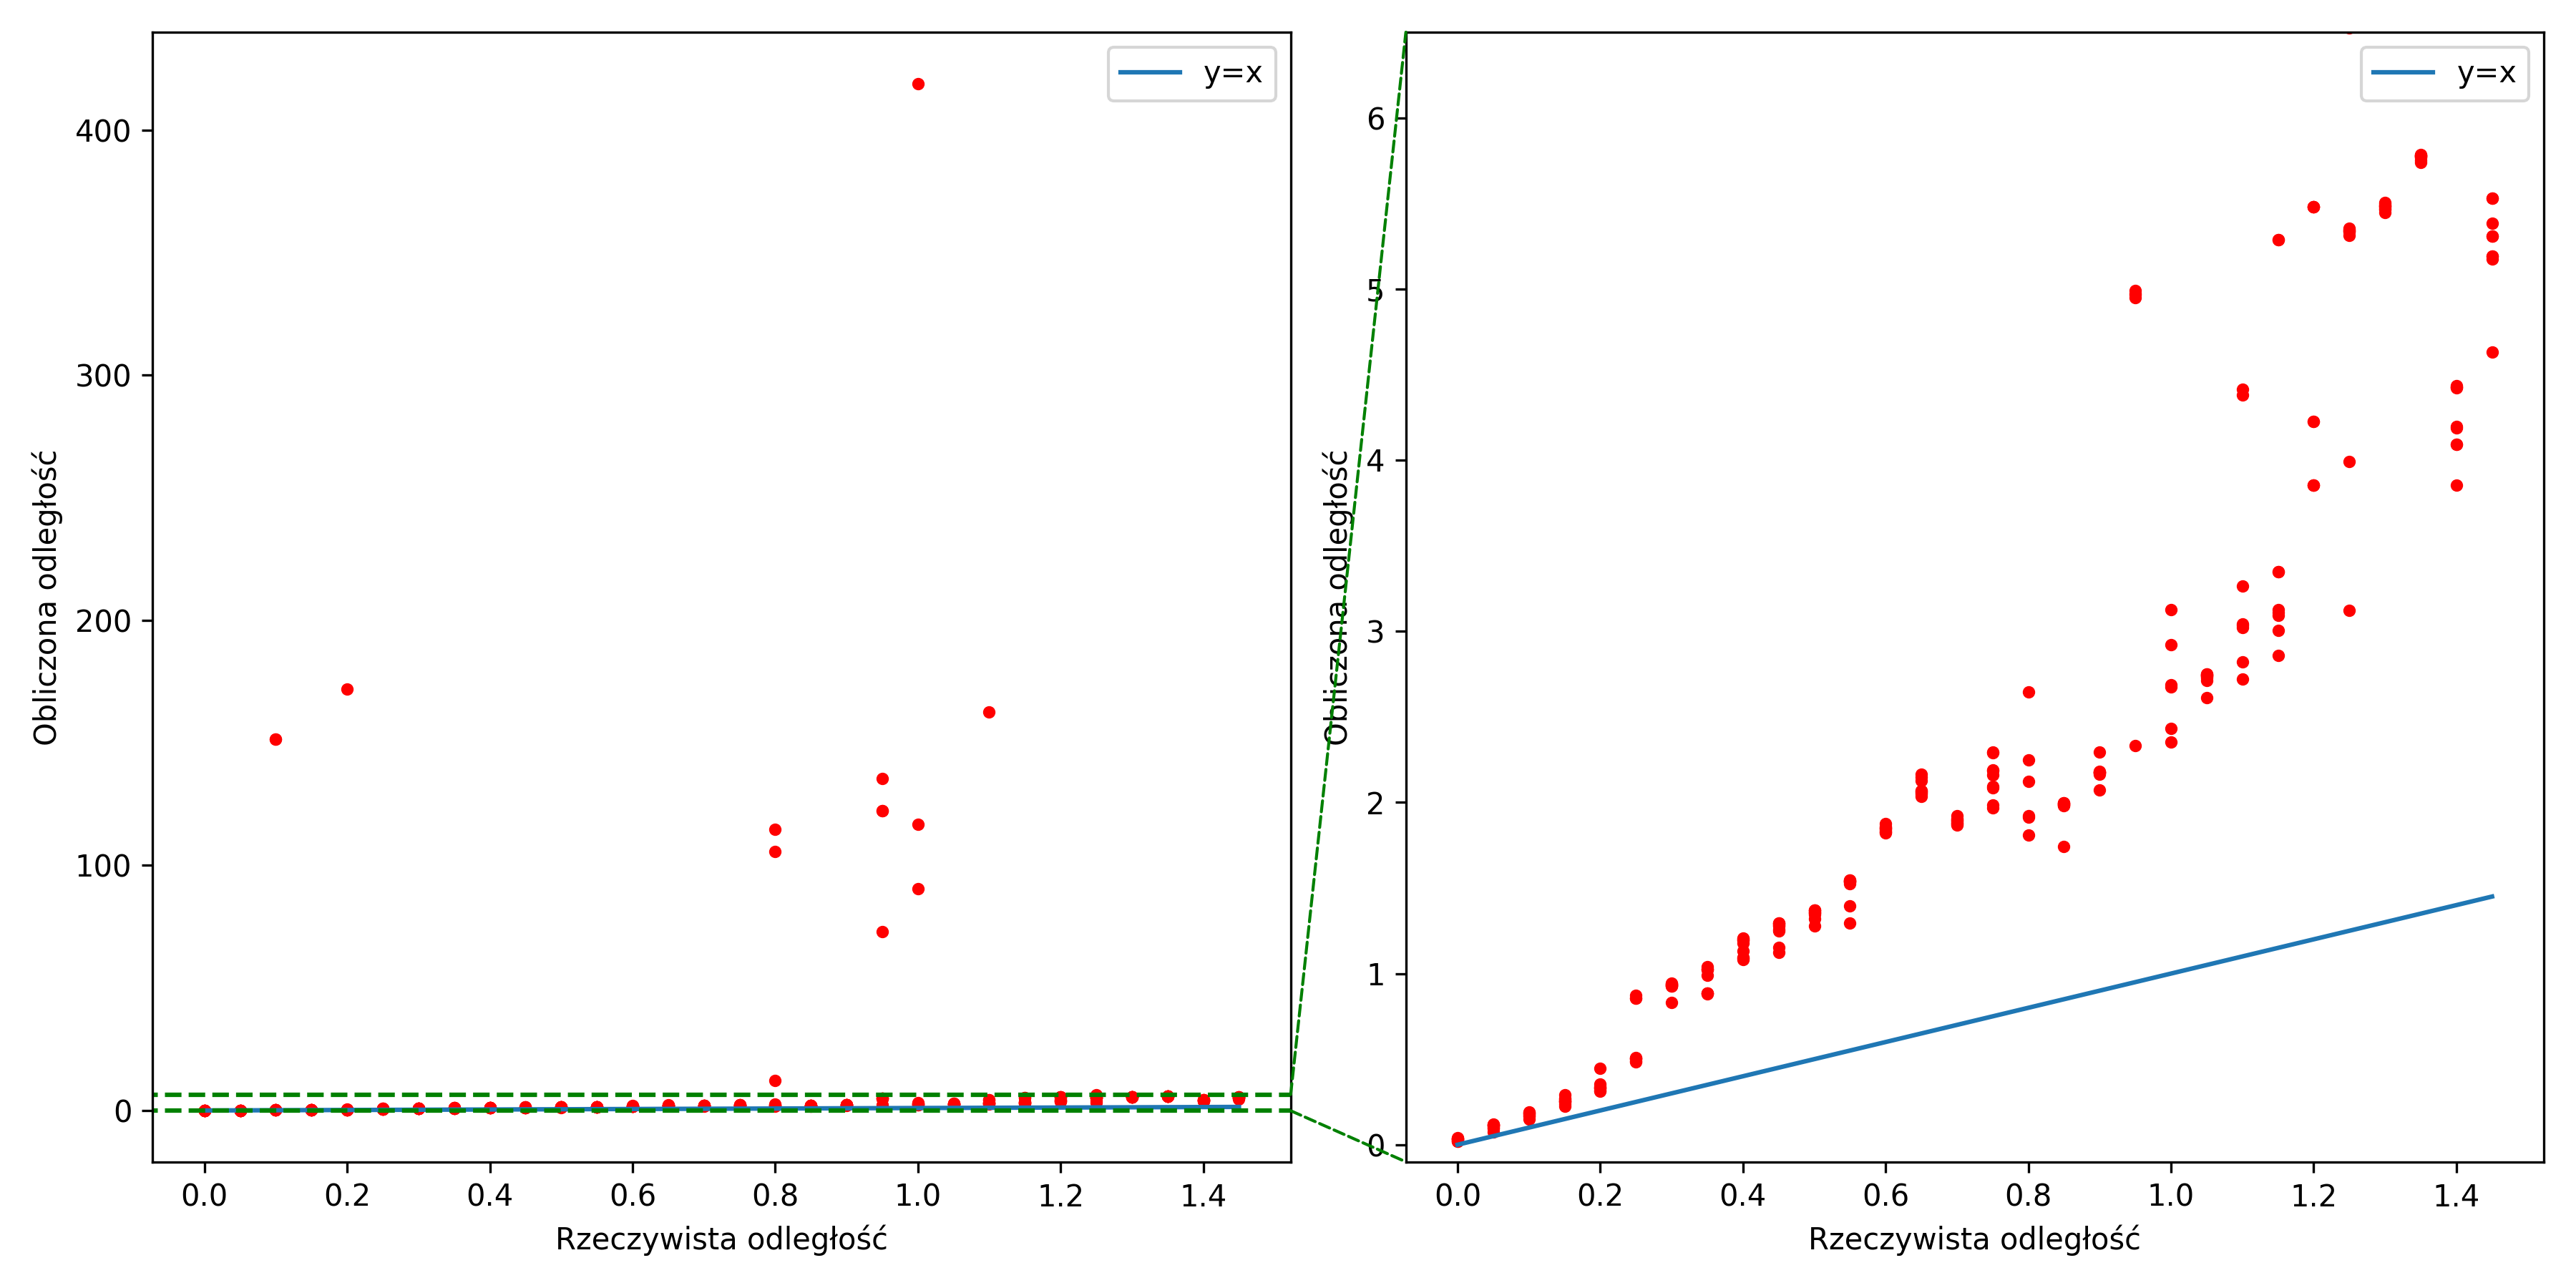
\includegraphics[width=.49\textwidth]{pics/mic_sync_dist/dists_long_3.png}
    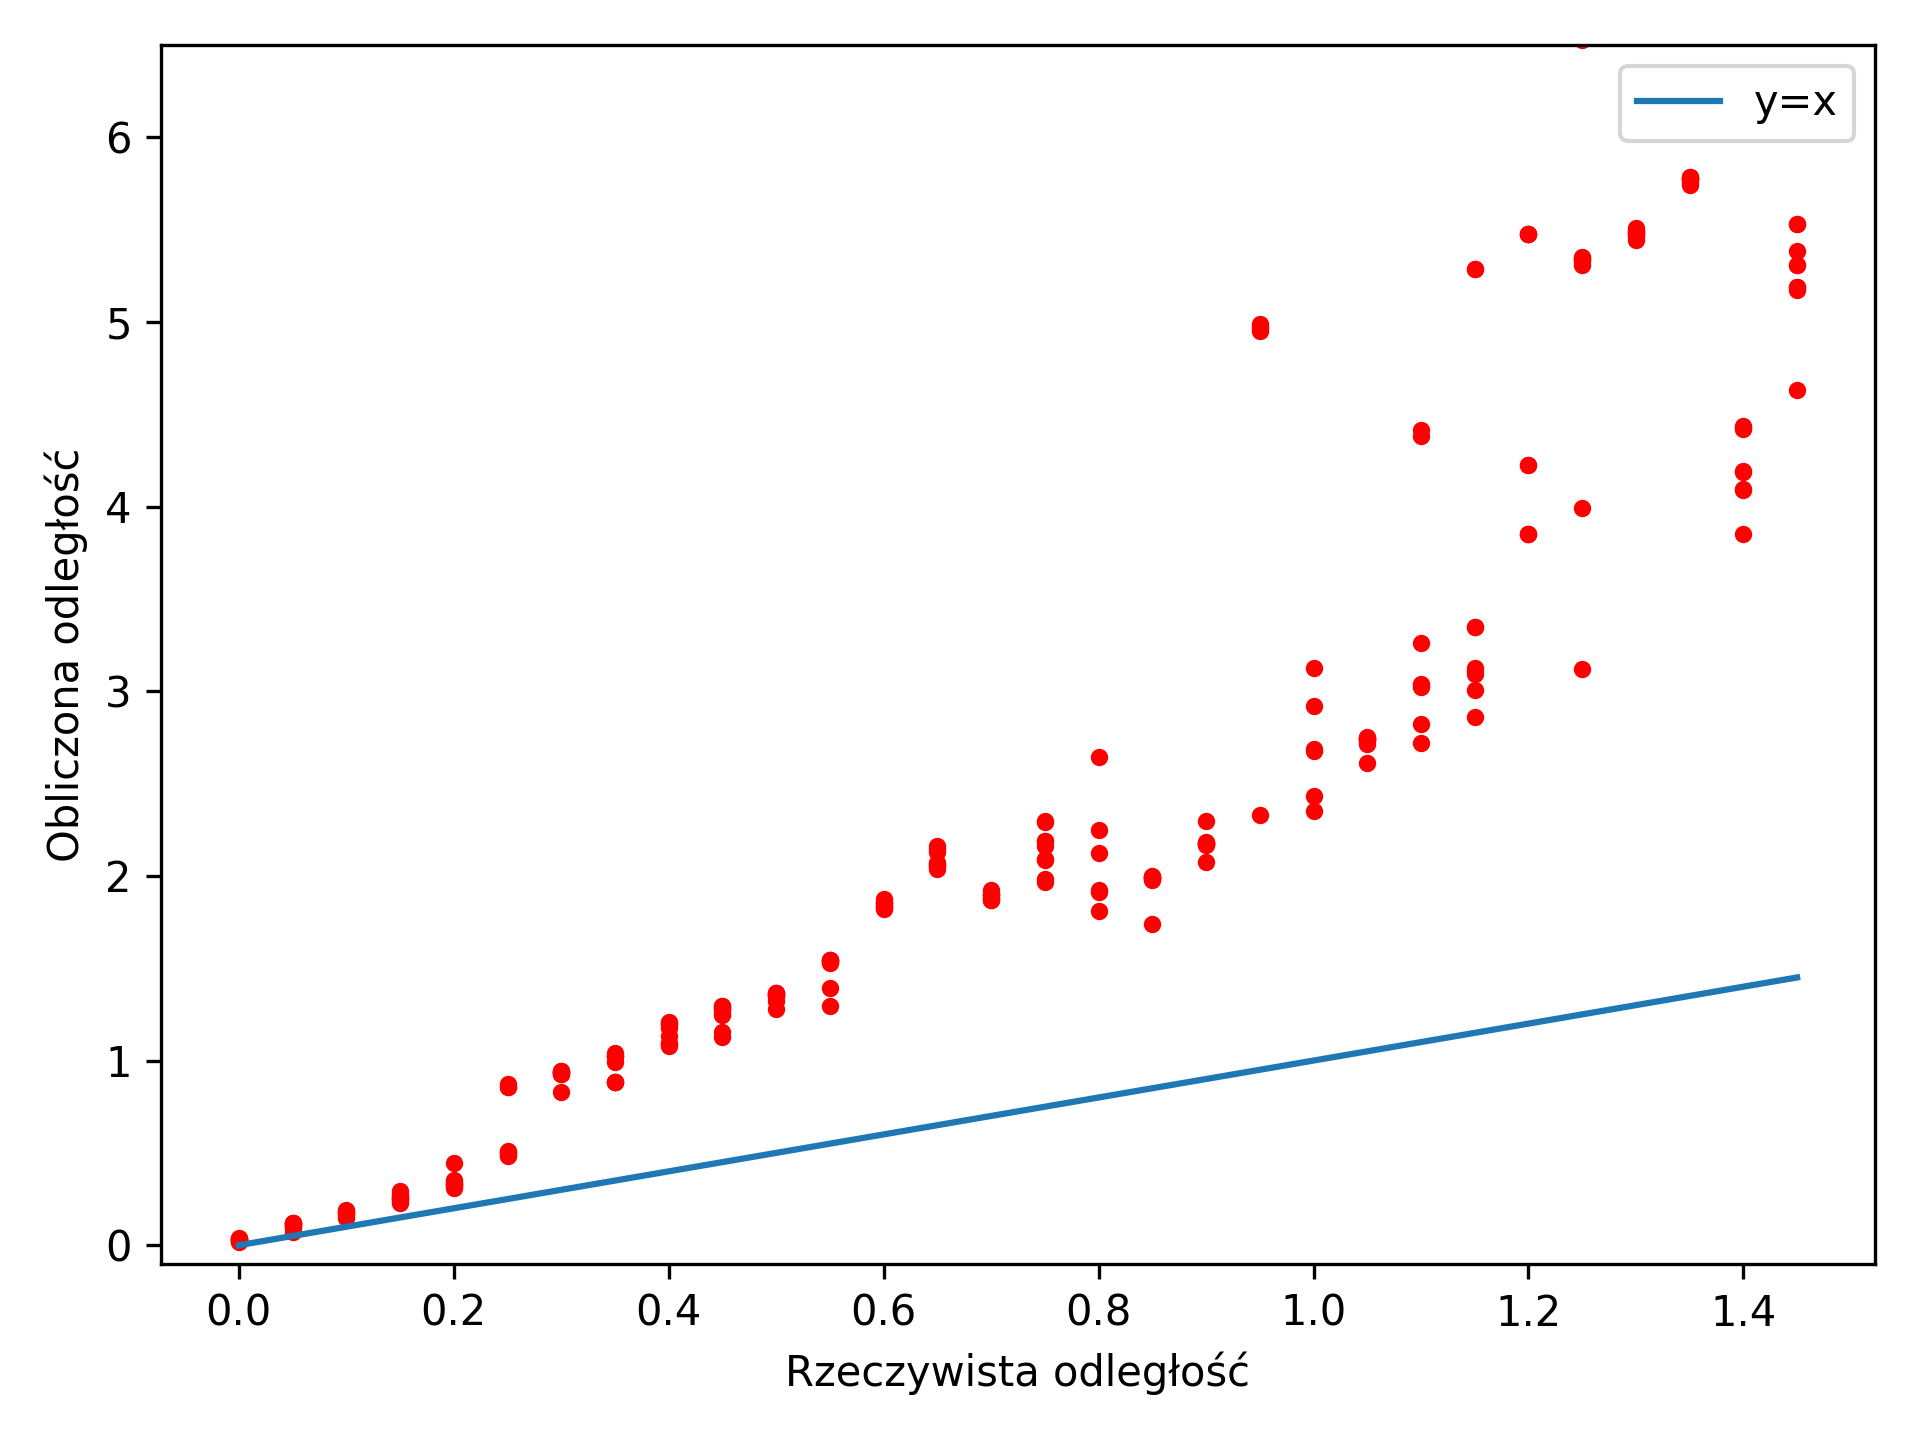
\includegraphics[width=.49\textwidth]{pics/mic_sync_dist/dists_close_long_3.png}
\caption{Pomiar obliczanych odległości 4.}
\label{pic:slope_test_3}
\end{figure}

Aby lepiej odczytać informacje z wykresu uśrednijmy pomiary dla każdej z badanych odległości i dodajmy do nich funkcje liniowe o współczynniku otrzymanym przy pomocy regresji liniowej z tychże uśrednionych punktów.

\begin{figure}[h]
\centering
    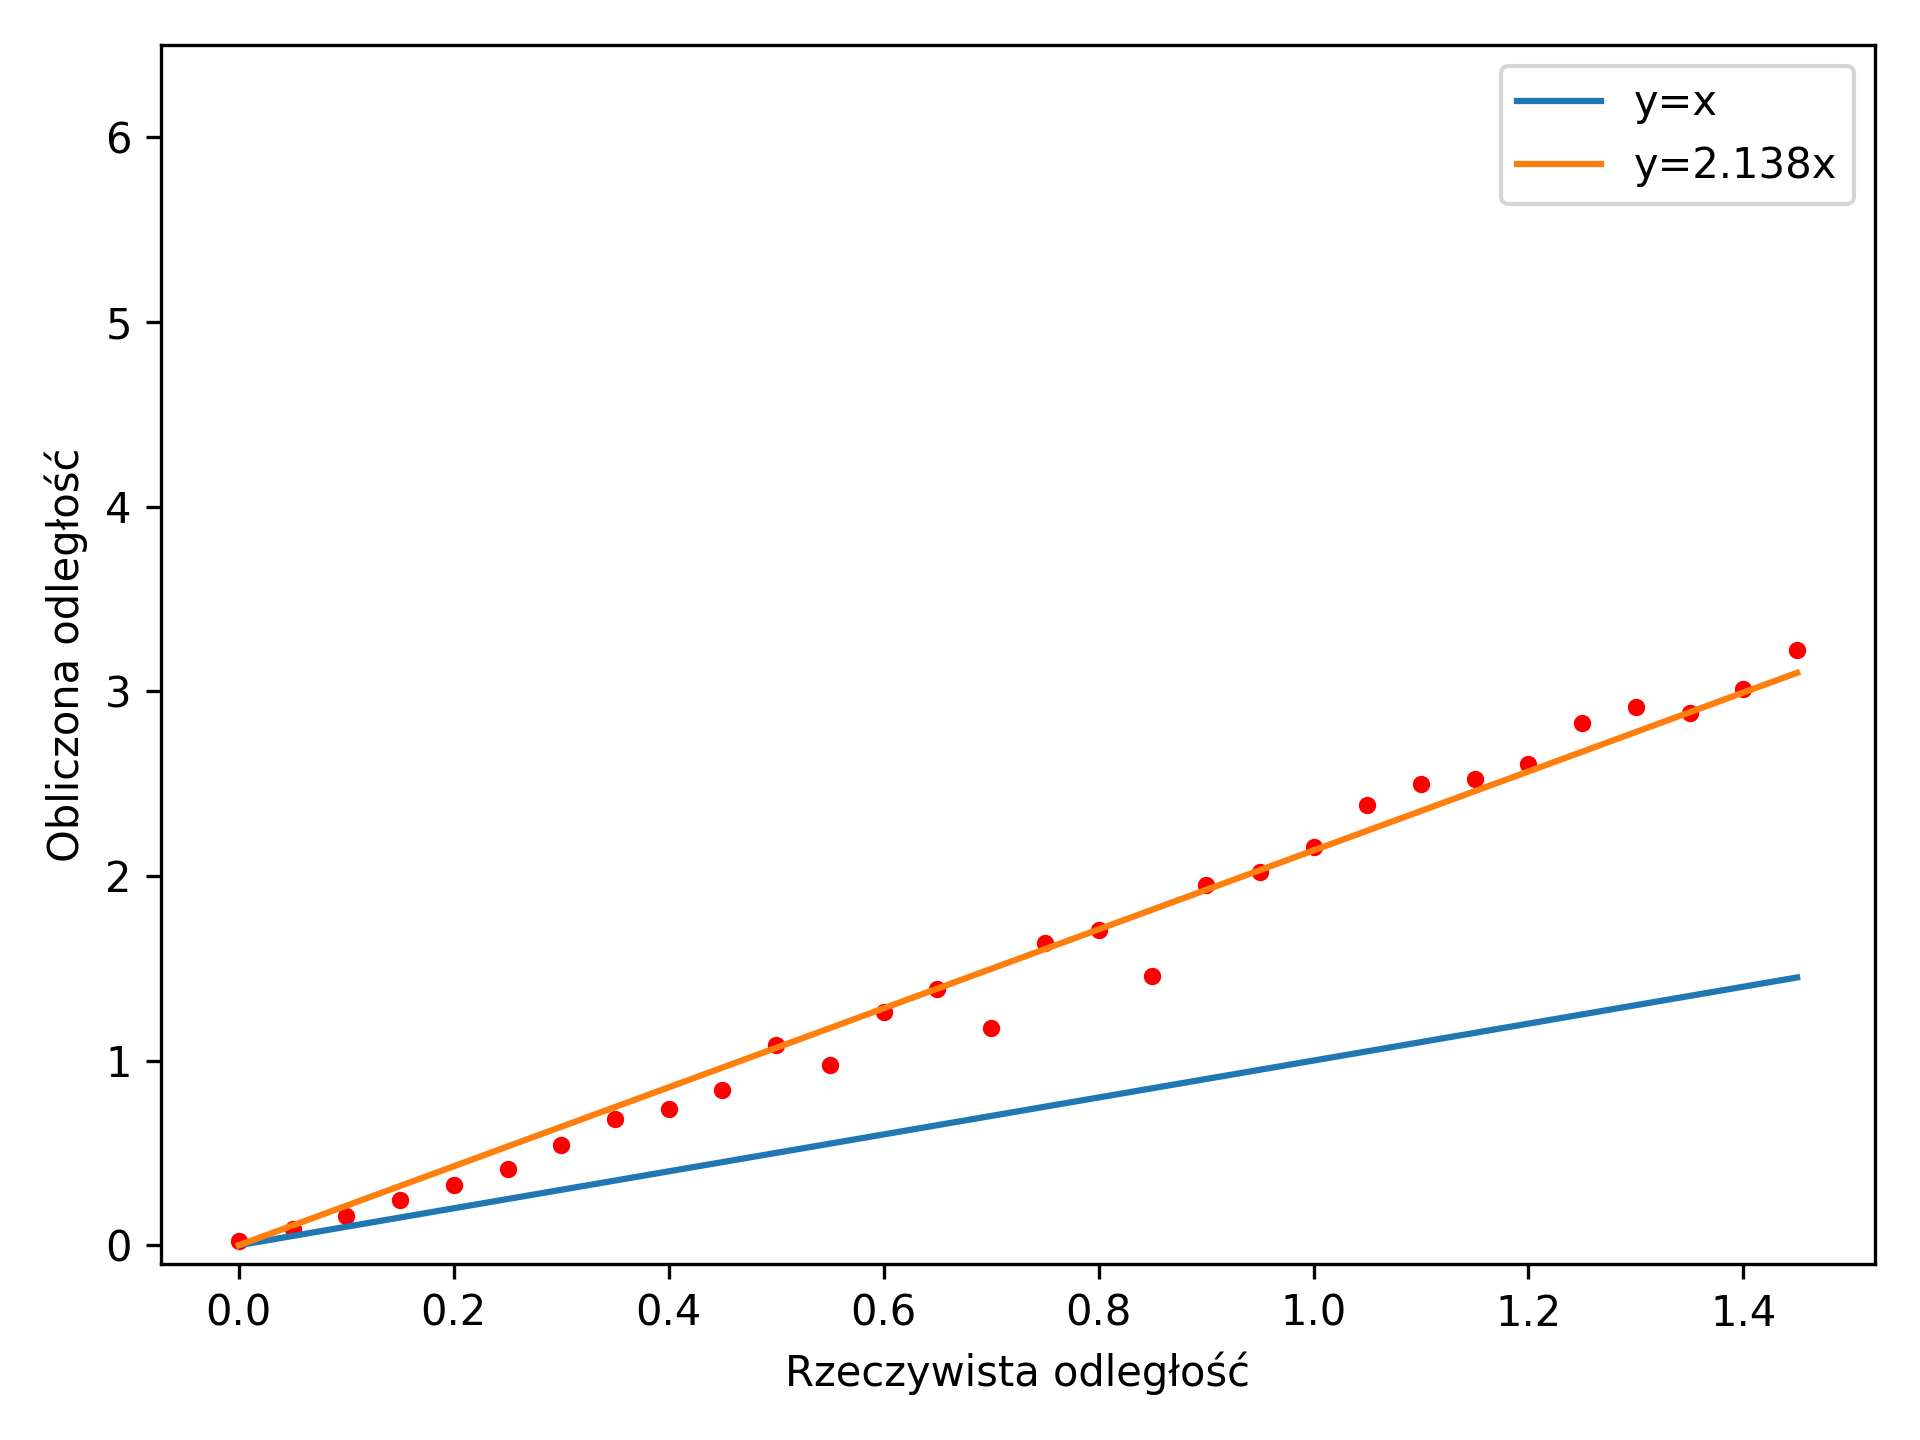
\includegraphics[width=.49\textwidth]{pics/mic_sync_dist/dists_close_long_0_mean.png}
    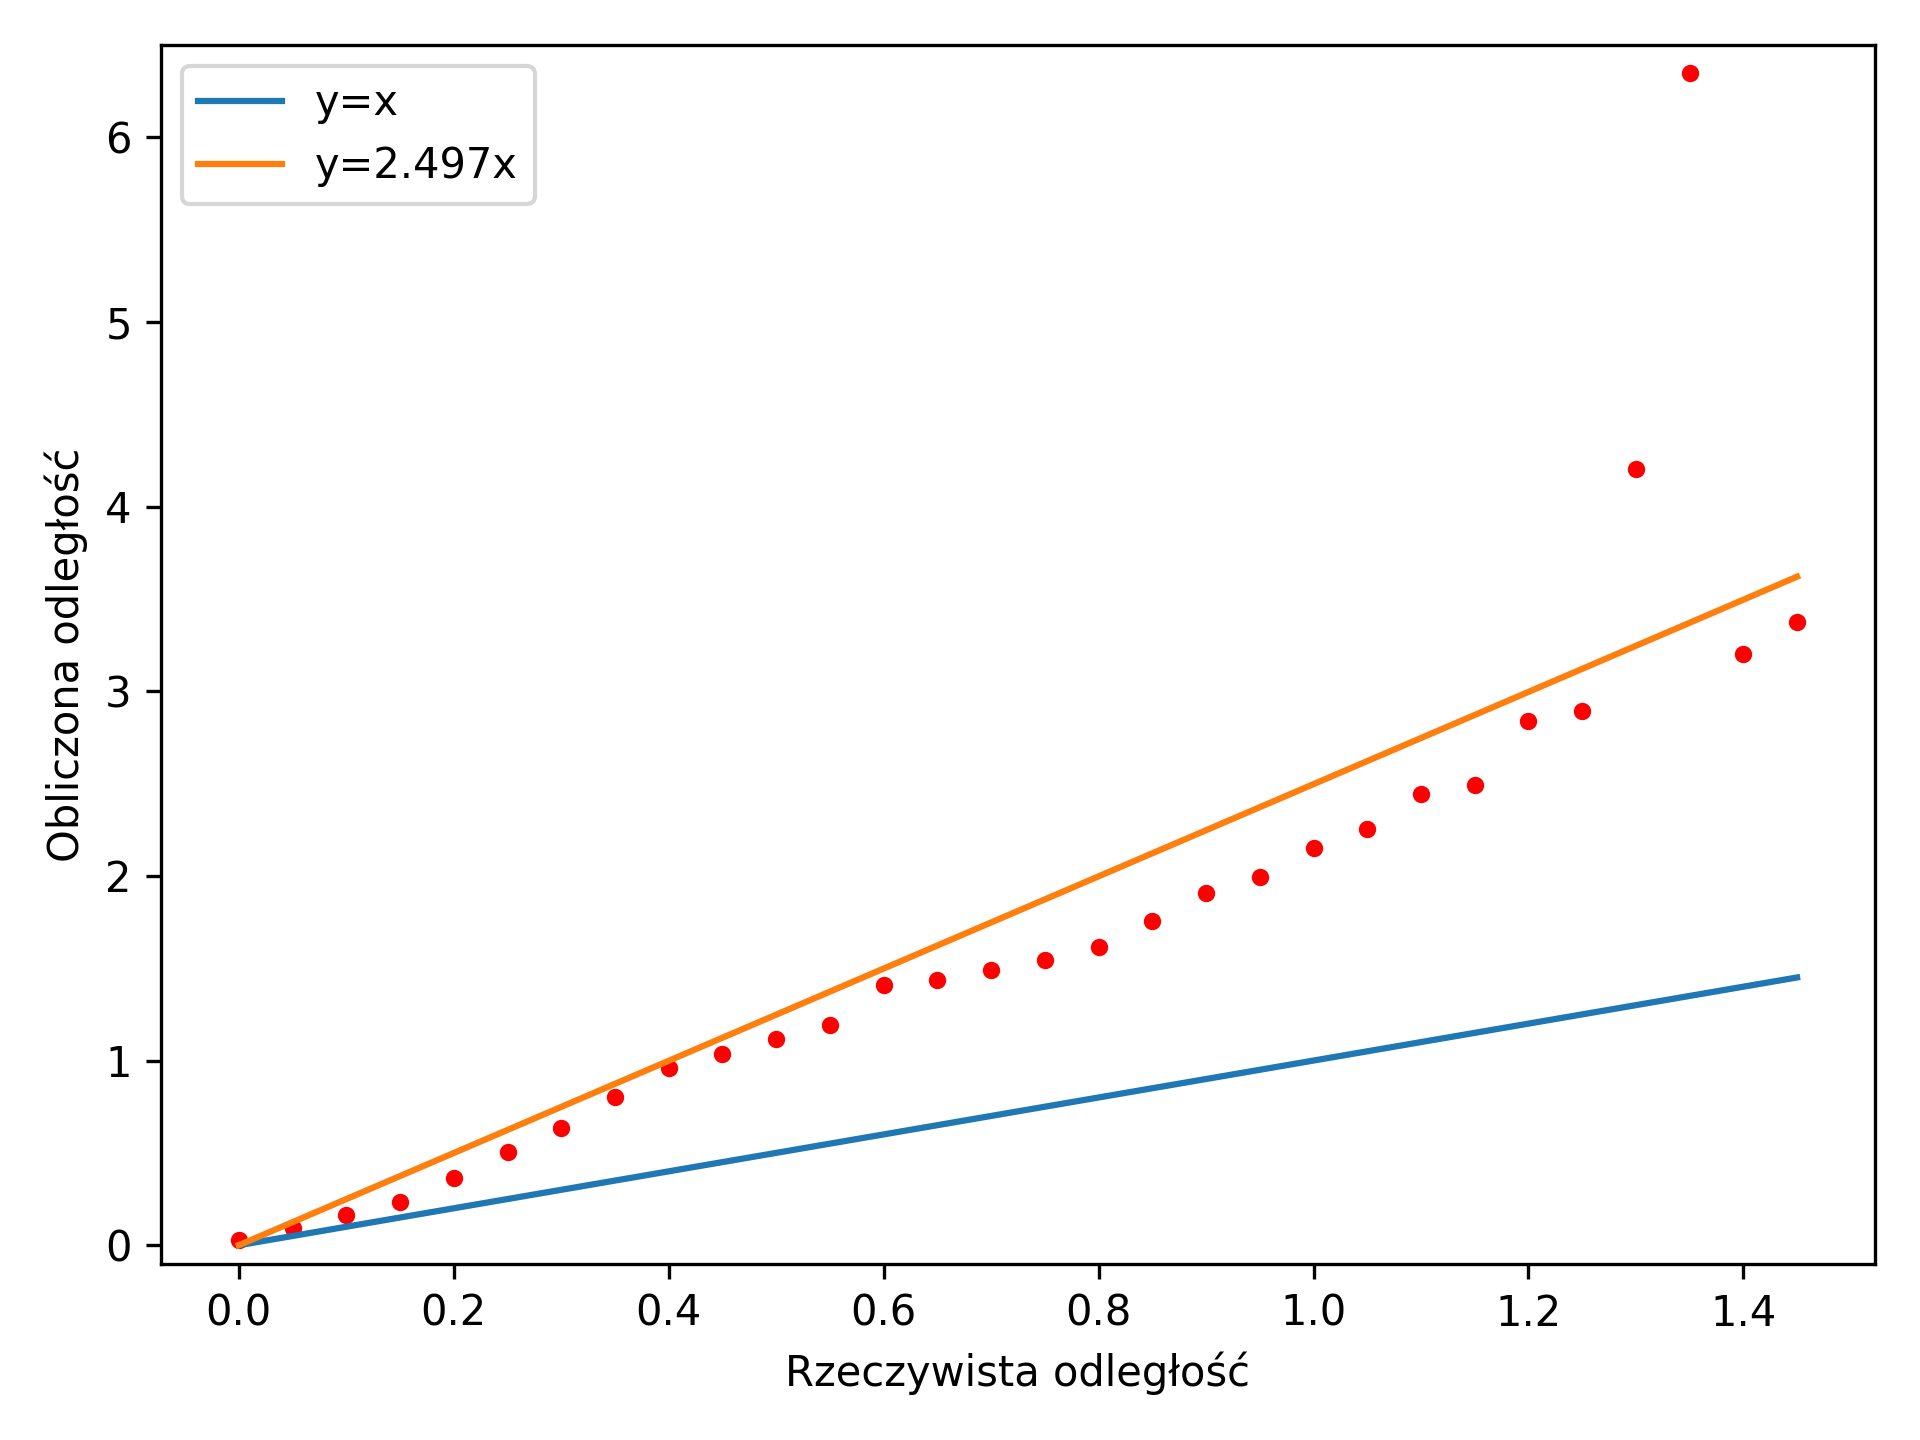
\includegraphics[width=.49\textwidth]{pics/mic_sync_dist/dists_close_long_1_mean.png}
    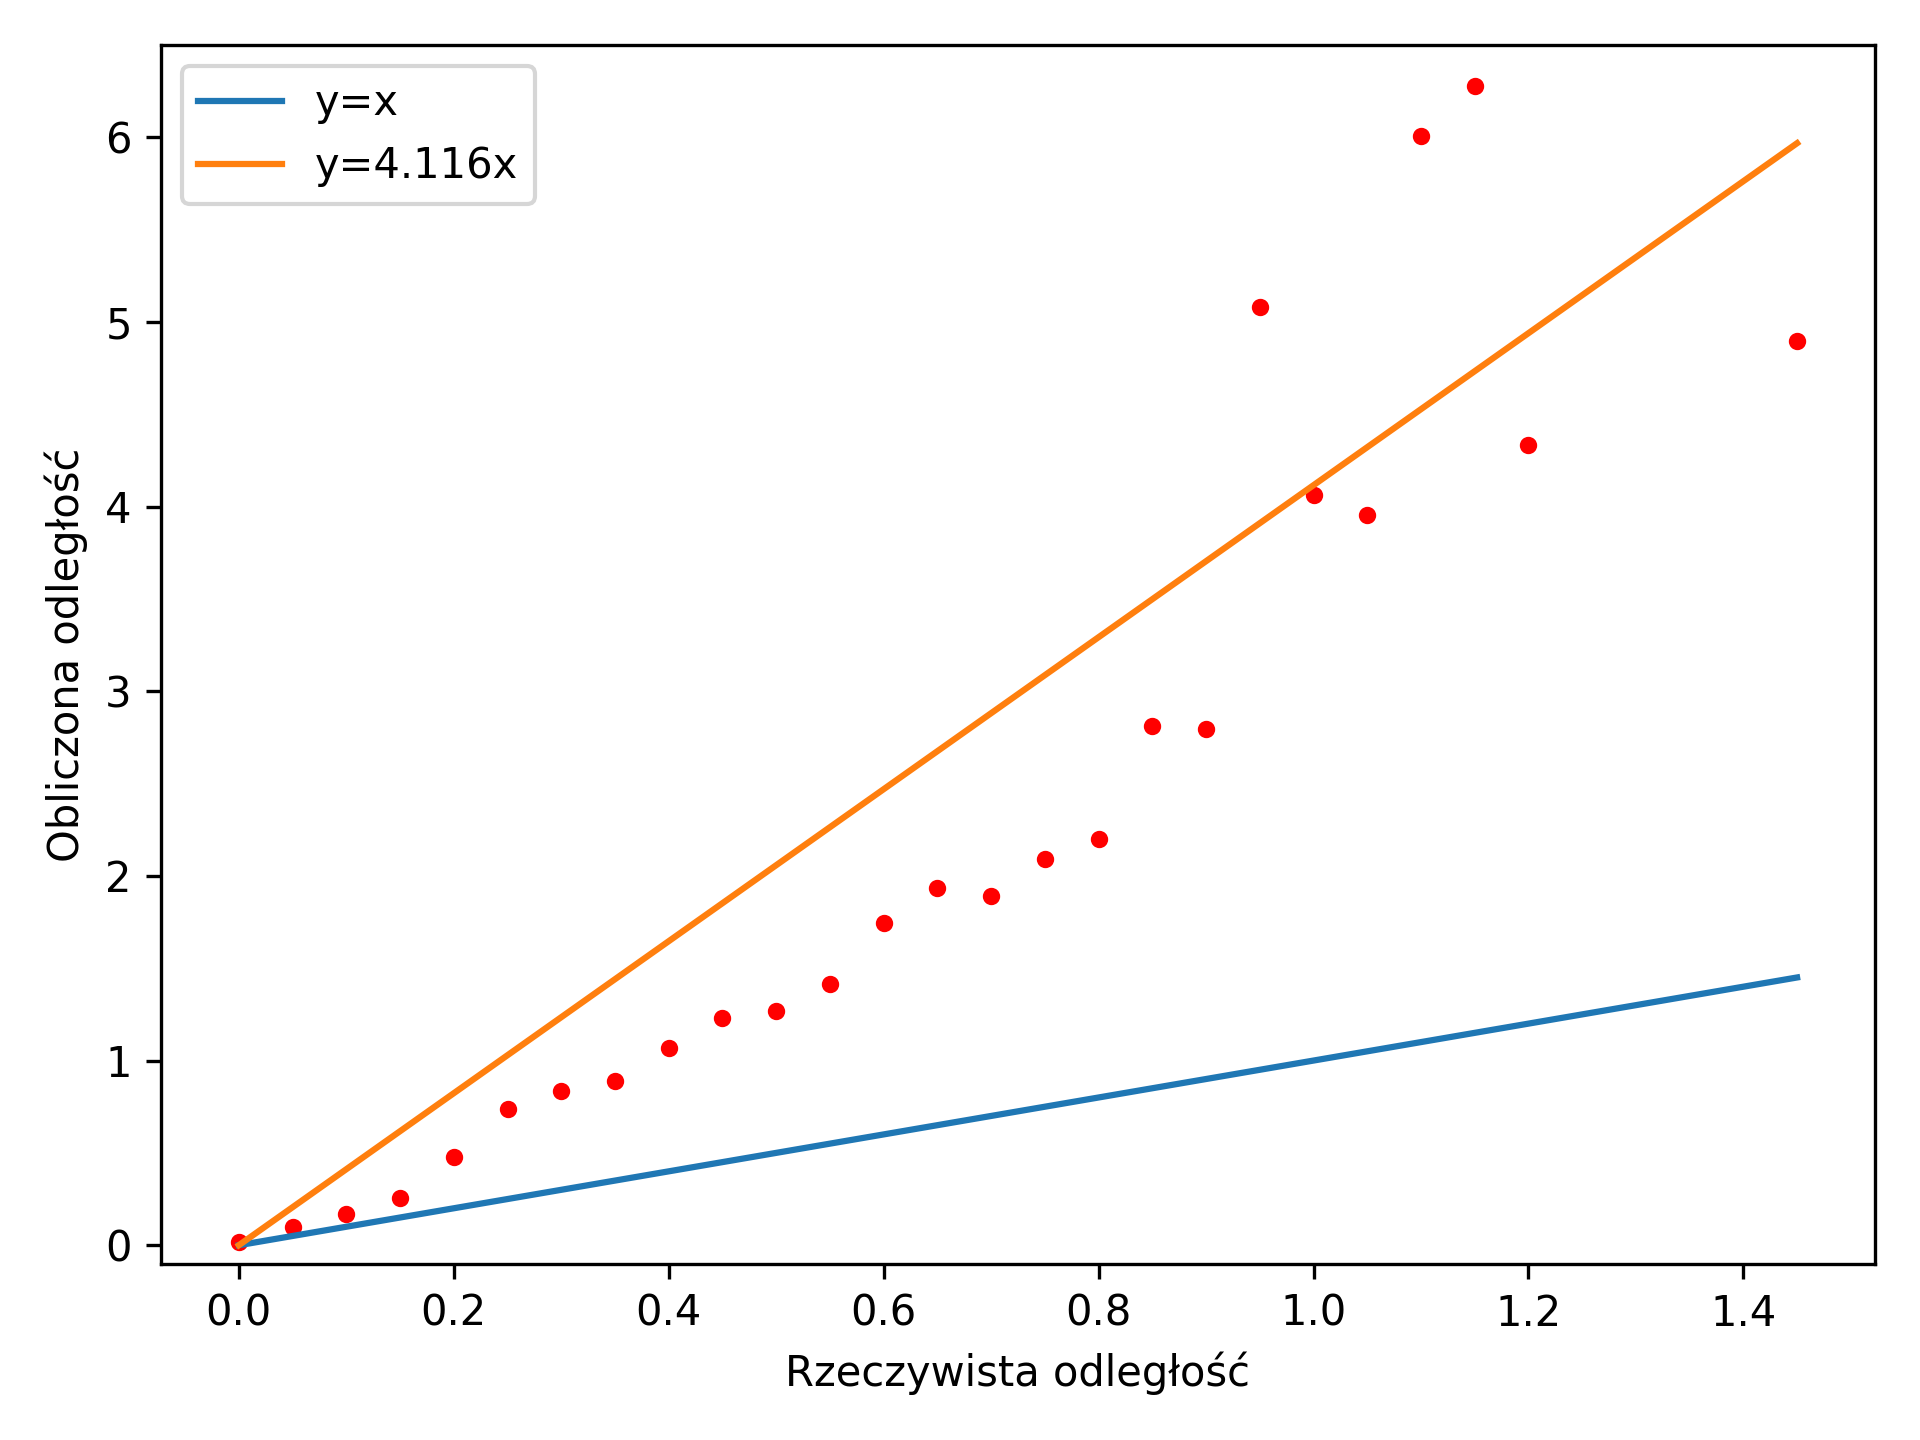
\includegraphics[width=.49\textwidth]{pics/mic_sync_dist/dists_close_long_2_mean.png}
    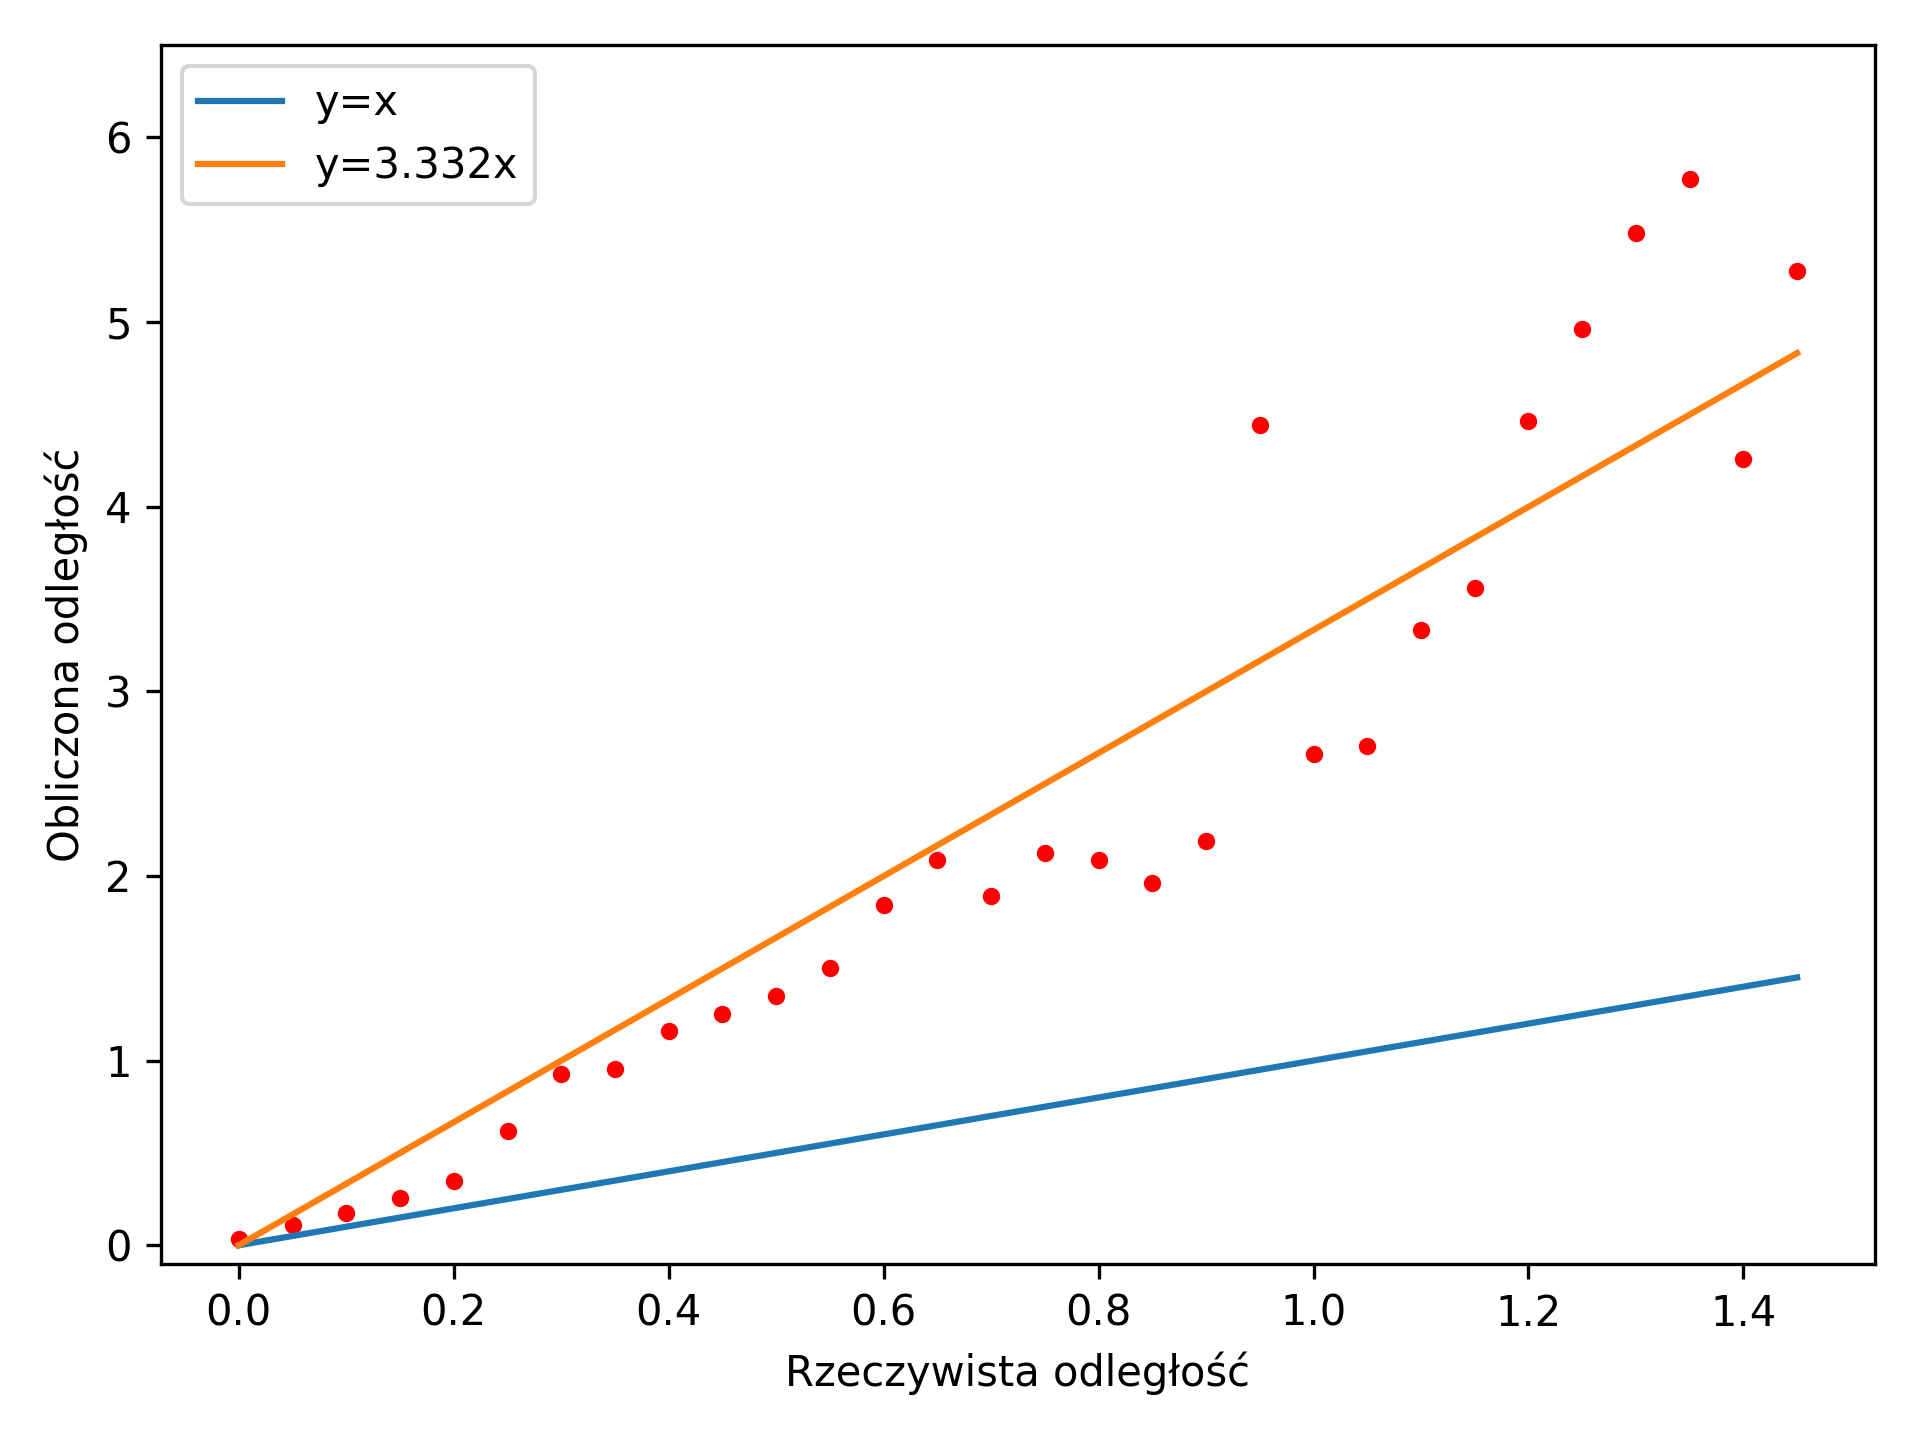
\includegraphics[width=.49\textwidth]{pics/mic_sync_dist/dists_close_long_3_mean.png}
\caption{Średnie obliczonych odległości}
\label{pic:slope_test_mean}
\end{figure}

Na wykresach można zauważyć trendy związane ze zmniejszającą się czułością wzmacniacza mikrofonu:

\begin{itemize}
    \item zmniejszanie się odległości punktu, w którym czułość jest zbyt mała by niezawodnie wyrywać nadawane sygnały,
    \item współczynnik prostej aproksymującej skalowane odległości rośnie.
\end{itemize}

Podobne efekty zaobserwowano kiedy brzęczyk nie był kierowany bezpośrednio w kierunku odbiornika.

\section{Ewaluacja działania systemu}

W celu ewaluacji działania przeprowadzono szereg eksperymentów testujących działanie systemu multilateracyjnego w zaproponowanych scenariuszach. Bazując na uprzednich obserwacjach rozszerzono program serwera obliczeniowego tak, aby bezpośrednio przed multilateracją przeprowadzone były synchronizacja czasu oraz korekcja odległości. Zasada działania obu typów węzłów pozostała niezmieniona.

\subsection{Wyniki}

Wyniki eksperymentów przedstawiono na wykresach. Mniejsze punkty o wyblakłym kolorze reprezentują badane punkty, w których umieszczony był węzeł nadawczy, natomiast większe, nasyconym kolorze odpowiadające im punkty będące uśrednionym wynikiem 25 powtórzeń polecenia lokalizacji w systemie. Wykresy należące do tej samej grupy zachowują skalę w celu łatwiejszego porównania.

\subsubsection{Eksperymeny jednowymiarowe}

Ewaluację rozpoczęto, tak jak podczas eksperymentu zerowego, od przypadku jednowymiarowego, aby sprawdzić czy dokładność i stabilność pomiarów w systemie została poprawiona. Tak samo jak pierwotnie nadajnik umiejscowiono w punkcie $(0)$, natomiast dwa odbiorniki w punktach odpowiednio $(-0.5)$ i $(0.5)$, wszystkie węzły były stacjonarne. Nadajnik co $0.5$ $s$ nadawał sygnał o długości $10$ $ms$, a serwer co $0.5$ $s$ zwracał wynik zagadnienia multilateracji na podstawie ostatnio otrzymanych danych. Następnie powtórzono eksperyment z użyciem dwóch dodatkowych węzłów umiejscowionych w punktach $(-0.25)$ i $(0.25)$. Wyniki przedstawiono na wykresach~\ref{pic:1d_mult}.

\begin{figure}[h]
\centering
\begin{subfigure}{.5\textwidth}
    \centering
    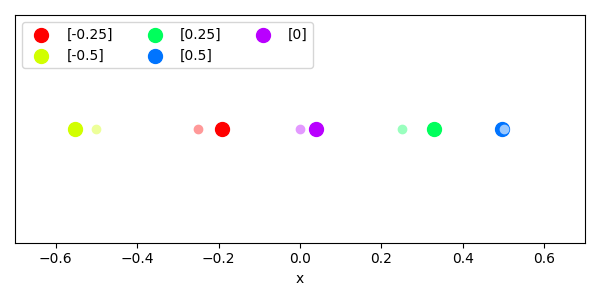
\includegraphics[width=\linewidth]{pics/mult_lat_1d/positions_2_mean.png}
\caption{2 węzły}
\label{pic:1d_2_mult}
\end{subfigure}%
\begin{subfigure}{.5\textwidth}
    \centering
    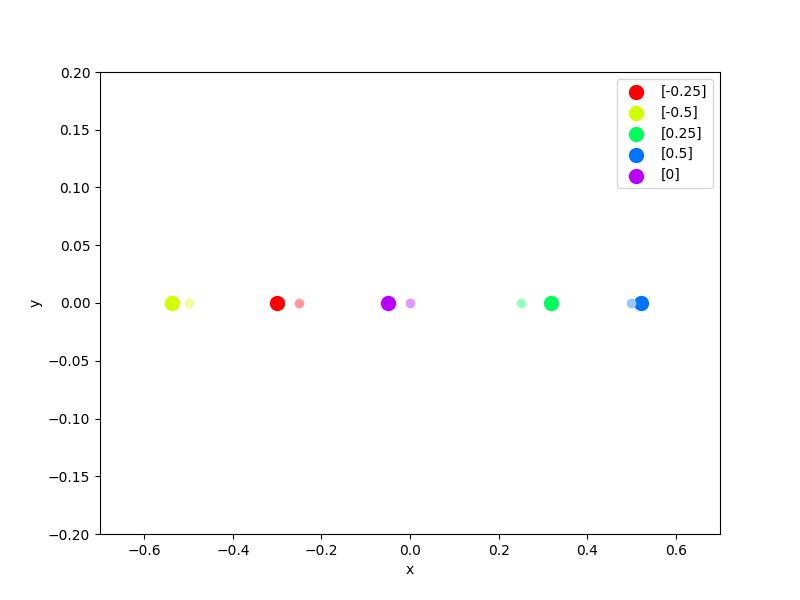
\includegraphics[width=\linewidth]{pics/mult_lat_1d/positions_4_mean.png}
    \caption{4 węzły}
\label{pic:1d_4_mult}
\end{subfigure}
\caption{Średnie obliczonych pozycji, wariant 1D}
\label{pic:1d_mult}
\end{figure}

\subsubsection{Eksperymeny dwuwymiarowe}

Następnie sprawdzono system w wariancie dwuwymiarowym. Zby zachować podobną maksymalną odległość pomiędzy odbiornikami zdecydowano na umiejscowienie czterech węzłów na wierzchołkach kwadratu o boku $0.6$ symetrycznego względem puntu $(0,0)$, a więc na punktach o współrzędnych $(\pm0.3, \pm0.3)$. Zbadano dokładność lokalizacji w trzech grupach punktów:
\begin{itemize}
    \item $\{(0,0), (0.3,0.3), (-0.3,0.3), (-0.3,-0.3), (0.3,-0.3)\}$
    \item $\{(0,0), (0,0.3), (0,-0.3), (-0.3,0), (0.3,0)\}$
    \item $\{(0,0), (0.15,0.15), (-0.15,0.15), (-0.15,-0.15), (0.15,-0.15)\}$
\end{itemize}
Wyniki przedstawiono na wykresach~\ref{pic:2d_mult}.

\begin{figure}[h]
\centering
\begin{subfigure}{.5\textwidth}
    \centering
    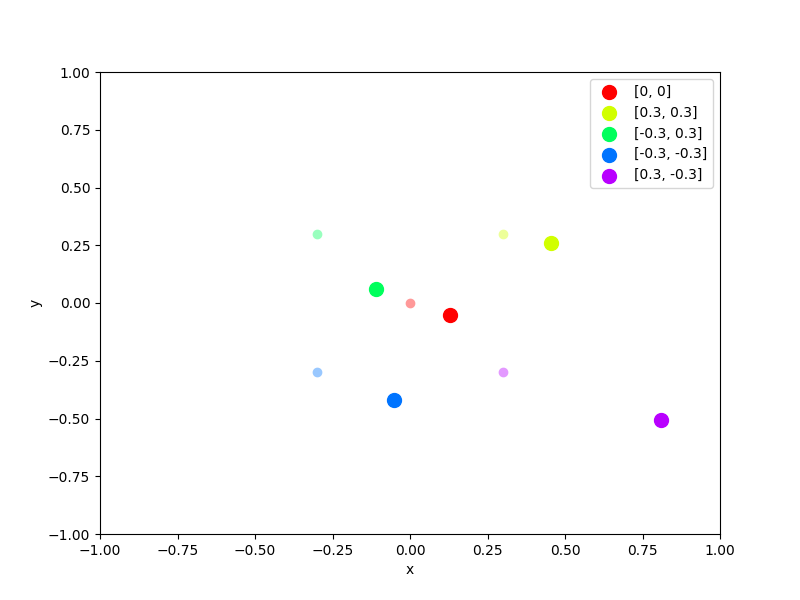
\includegraphics[width=\linewidth]{pics/mult_lat_2d/positions_1_mean.png}
\caption{zestaw punktów 1.}
\label{pic:2d_1_mult}
\end{subfigure}%
\begin{subfigure}{.5\textwidth}
    \centering
    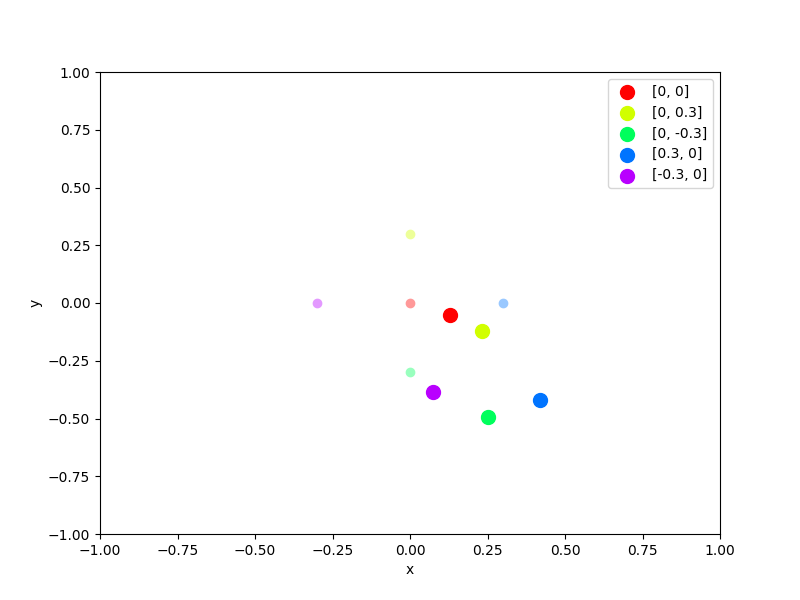
\includegraphics[width=\linewidth]{pics/mult_lat_2d/positions_2_mean.png}
\caption{zestaw punktów 2.}
\label{pic:2d_2_mult}
\end{subfigure}
\begin{subfigure}{.5\textwidth}
    \centering
    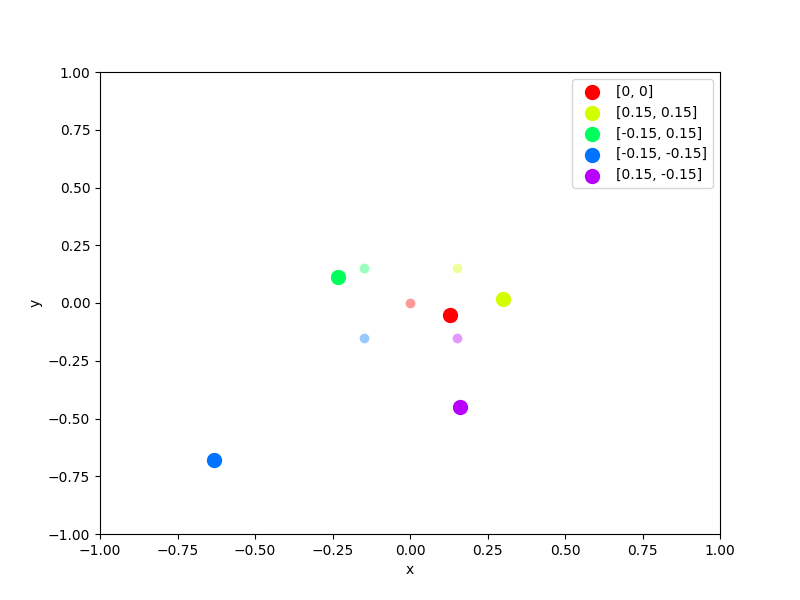
\includegraphics[width=\linewidth]{pics/mult_lat_2d/positions_3_mean.png}
\caption{zestaw punktów 3.}
\label{pic:2d_3_mult}
\end{subfigure}
\caption{Średnie obliczonych pozycji, wariant 2D}
\label{pic:2d_mult}
\end{figure}

Następnie w celu ewaluacji wpływu charakterystyki otoczenia na działanie systemu przeprowadzono trzy następujące bezpośrednio po sobie eksperymenty zachowując ustaloną na początku synchronizację zegarów i stałe korekcji odległości. Sprawdzono dokładność estymacji tego samego zbioru punktów wyjściowo oraz po rotacji całego układu o $45^{\circ}$ i $90^{\circ}$ zgodnie z ruchem wskazówek zegara. Wyniki przedstawiono na wykresach~\ref{pic:2d_angle_mult}. 

\begin{figure}[h]
\centering
\begin{subfigure}{.5\textwidth}
    \centering
    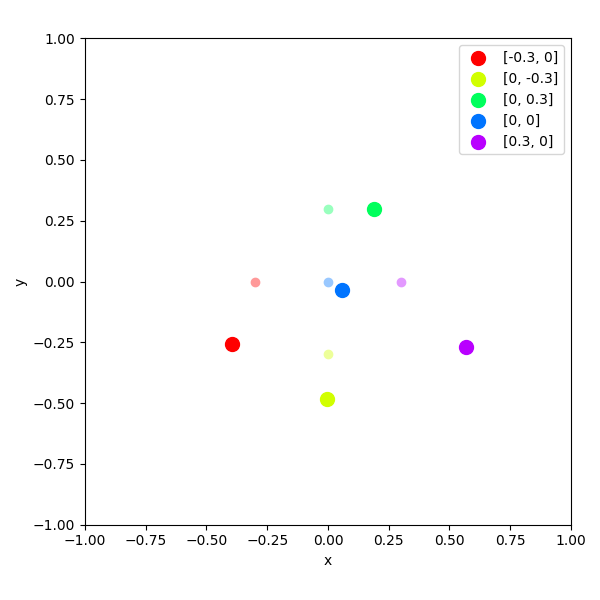
\includegraphics[width=\linewidth]{pics/mult_lat_2d_angle/positions_0_mean.png}
\caption{rotacja $0^{\circ}$}
\label{pic:2d_0_angle_mult}
\end{subfigure}%
\begin{subfigure}{.5\textwidth}
    \centering
    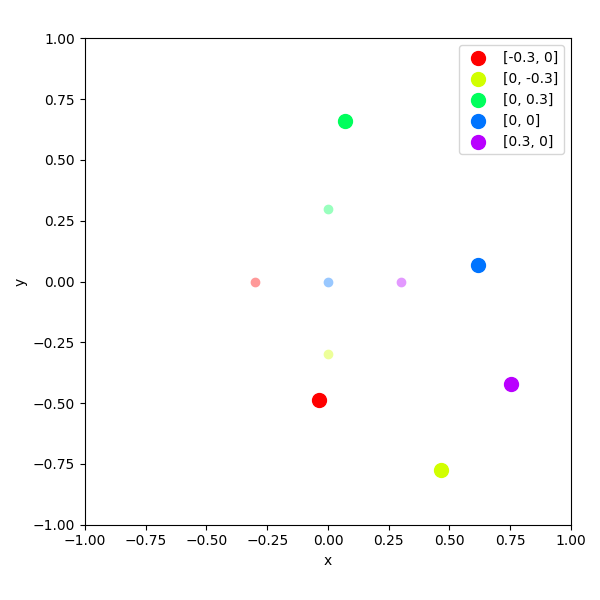
\includegraphics[width=\linewidth]{pics/mult_lat_2d_angle/positions_45_mean.png}
\caption{rotacja $45^{\circ}$}
\label{pic:2d_45_angle_mult}
\end{subfigure}
\begin{subfigure}{.5\textwidth}
    \centering
    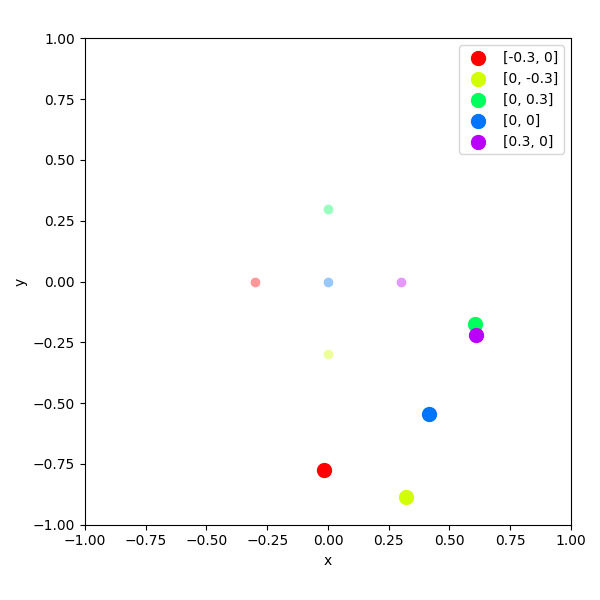
\includegraphics[width=\linewidth]{pics/mult_lat_2d_angle/positions_90_mean.png}
\caption{rotacja $90^{\circ}$}
\label{pic:2d_90_angle_mult}
\end{subfigure}
\caption{Średnie obliczonych pozycji, wariant 2D z rotacją}
\label{pic:2d_angle_mult}
\end{figure}

Ostatecznie sprawdzono zachowanie systemu wraz ze zmianą liczby węzłów odbiorczych od minimalnej liczby trzech aż do ośmiu. Węzły umiejscowiono na punktach ze zbioru $\{(0,0), (0.3,0.3), (-0.3,0.3), (-0.3,-0.3), (0.3,-0.3), (0, 0.425), (-0.425, 0), (0, -0.425), (0.425, 0)\}$ oraz dodawano je zgodnie z tą kolejnością. Wyniki przedstawiono na wykresach~\ref{pic:2d_num_mult}. 

\begin{figure}[h]
\centering
\begin{subfigure}{.5\textwidth}
    \centering
    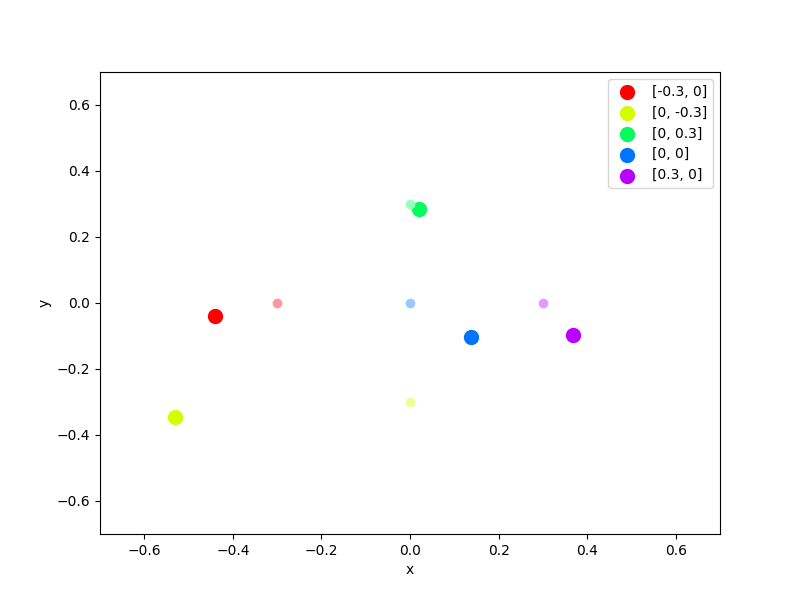
\includegraphics[width=\linewidth]{pics/mult_lat_2d_num/positions_3_mean.png}
\caption{3 węzły}
\label{pic:2d_3_num_mult}
\end{subfigure}%
\begin{subfigure}{.5\textwidth}
    \centering
    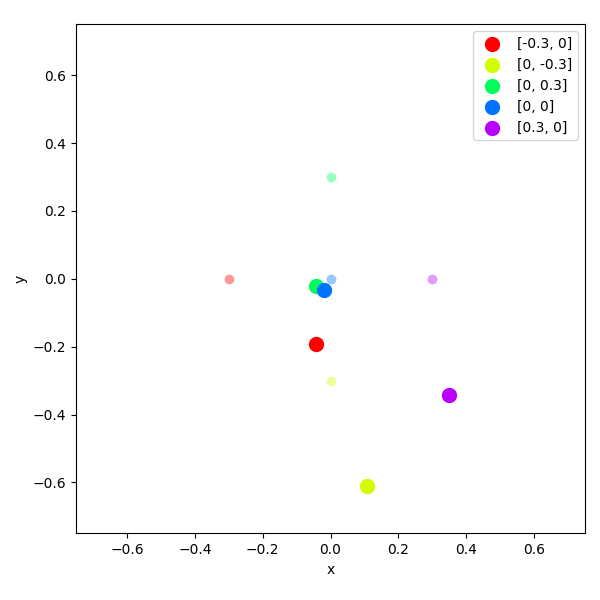
\includegraphics[width=\linewidth]{pics/mult_lat_2d_num/positions_4_mean.png}
\caption{4 węzły}
\label{pic:2d_4_num_mult}
\end{subfigure}
\begin{subfigure}{.5\textwidth}
    \centering
    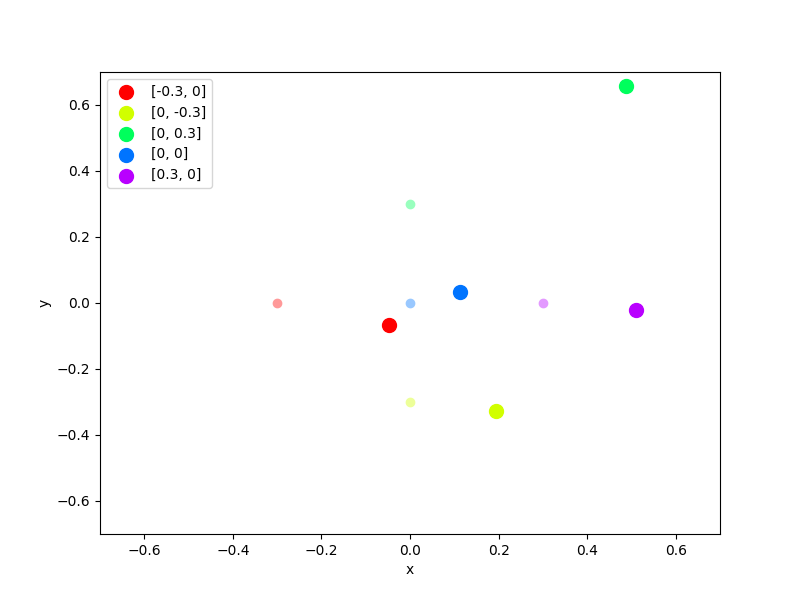
\includegraphics[width=\linewidth]{pics/mult_lat_2d_num/positions_5_mean.png}
\caption{5 węzłów}
\label{pic:2d_5_num_mult}
\end{subfigure}%
\begin{subfigure}{.5\textwidth}
    \centering
    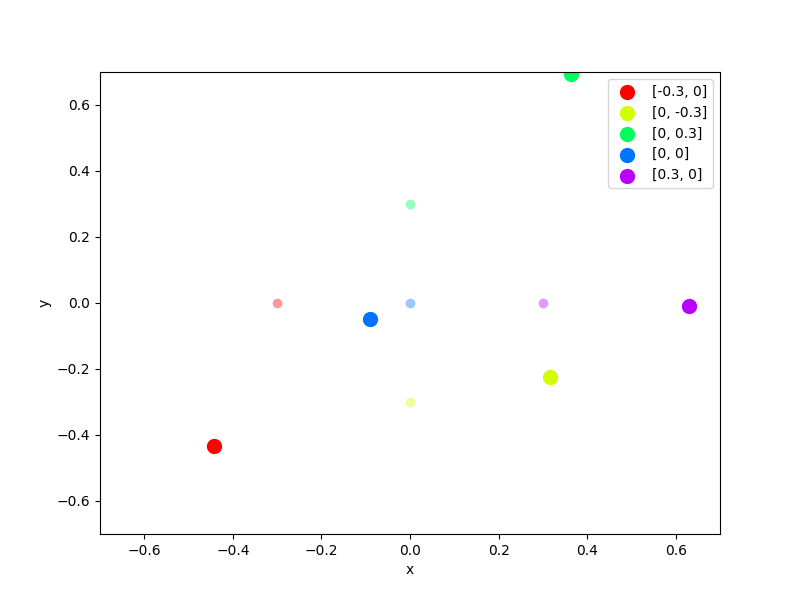
\includegraphics[width=\linewidth]{pics/mult_lat_2d_num/positions_6_mean.png}
\caption{6 węzłów}
\label{pic:2d_6_num_mult}
\end{subfigure}
\begin{subfigure}{.5\textwidth}
    \centering
    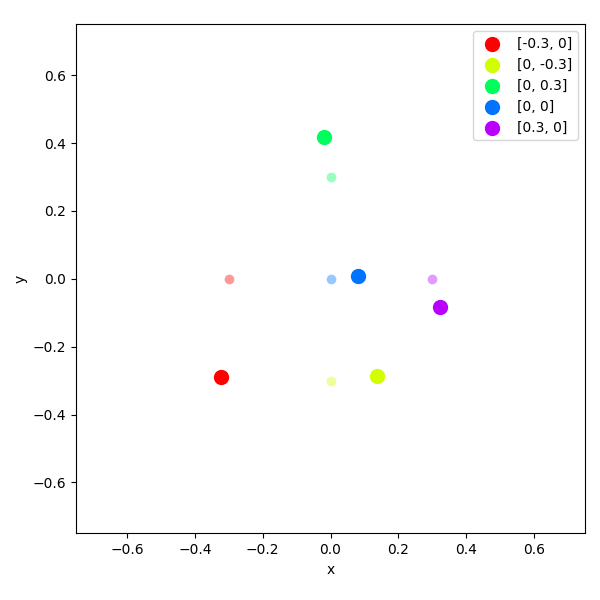
\includegraphics[width=\linewidth]{pics/mult_lat_2d_num/positions_7_mean.png}
\caption{7 węzłów}
\label{pic:2d_7_num_mult}
\end{subfigure}%
\begin{subfigure}{.5\textwidth}
    \centering
    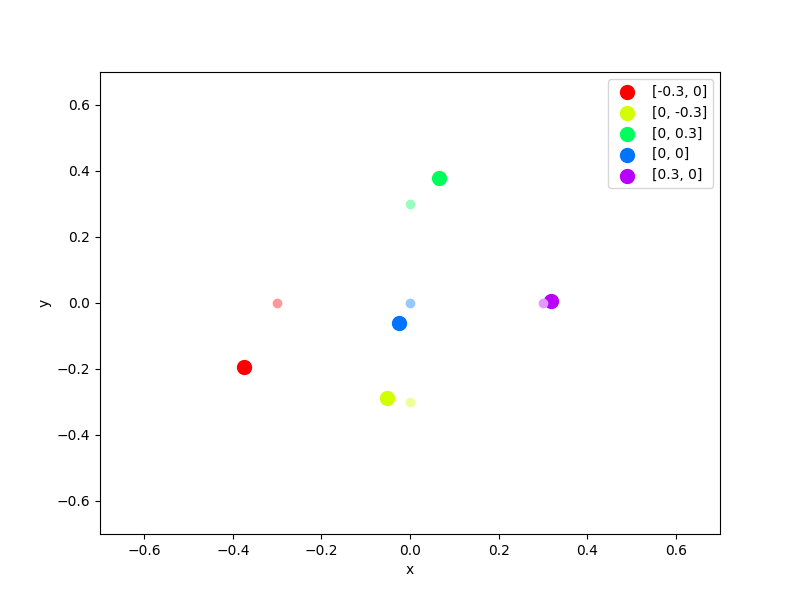
\includegraphics[width=\linewidth]{pics/mult_lat_2d_num/positions_8_mean.png}
\caption{8 węzłów}
\label{pic:2d_8_num_mult}
\end{subfigure}
\caption{Średnie obliczonych pozycji, wariant 2D ze zmienną liczbą węzłów}
\label{pic:2d_num_mult}
\end{figure}

\section{Interpretacja i wnioski}
\chapter*{Podsumowanie}\label{chap:podsumowanie}
\addcontentsline{toc}{chapter}{Podsumowanie}

Celem pracy niniejszej pracy było zaprojektowanie i zaimplementowanie systemu multilateracyjnego działającego w domenie fal dźwiękowych. W ramach pracy dokonano wyboru metody multilateracji najlepiej nadającej się do tego zastosowania, jak również przeprowadzono szereg testów wykazujących nieprawidłowości działania, a następnie podjęto próby eliminacji tych błędów. Podczas eksperymentów podstawową potrzebę dokładnej synchronizacji zegarów urządzeń w systemie na efekty jego działania. Przeanalizowano też znaczenie wpływu zastosowanej metody synchronizacji zegarów, a także interesujące skalowanie estymowanej odległości wynikającej z fizycznych mechanizmów rozchodzenia się fali dźwiękowej.

Wnioski z przeprowadzonych badań wskazują, że system multilateracyjny oparty o szeroko dostępne moduły mikrofonowe jest zdolny śledzić pozycję nadajnika sygnałów dźwiękowych w podzbiorze przestrzeni dwuwymiarowej obejmowanym ograniczonym zasięgiem tychże mikrofonów w węzłach odbiorczych. Uzyskane wyniki są istotne z punktu widzenia systemów lokalizacji bazujących na falach dźwiękowych, szczególnie w kontekście ich zastosowań w technologii IoT. Wykazano, że dostępne komercyjnie moduły mikrofonowe mogą być wykorzystane do tworzenia efektywnych i stosunkowo tanich systemów lokalizacji.

\color{blue}
wydaje się jednak, że szczyptę dziegciu warto by dodać i rzetelnie powiedzieć, że czasami może być niezły bałagan i dużo zależy od środowiska akustycznego... no i że nie wiadomo, jak to będzie się sprawować na większych odległościach -- może postawiłby Pan jakąś hipotezę?

może słówko jeszcze o wydajności (złożoności obliczeniowej) -- że małe urządzonka, a dają radę i w efekcie nie dość, że mikrofony za dwa złote, to jeszcze procesory za piątaka i wszystko działa (albo: prawie działa).
\color{black}

Dalszymi krokami rozwoju systemu, których nie podjęto ze względu na ograniczony budżet czasowy mogłyby być:

\begin{itemize}
    \item rozszerzenie do i ewaluacja działania w przestrzeni trójwymiarowej,
    \item bardziej wnikliwe testy i badania roli urządzeń przetwarzających sygnał dźwiękowy na cyfrowy; inwestygacja wpływu typu rodzaju mikrofonu, wzmacniacza czy przetwornika ADC (\textit{ang.\ analog to digital}) na estymację odległości,
    \item stworzenie lepszego algorytmu korekcji estymowanej odległości względem rzeczywistej,
    \item ewentualne dostosowywanie algorytmów synchronizacji zegarów do przyszłych zastosowań,
    \item próba minimalizacji wpływu charakterystyki dźwiękowej otoczenia na dokładność wyników.
\end{itemize}

Podsumowując, zaprojektowany i zaimplementowany system multilateracyjny działający w domenie fal dźwiękowych udowodnił swoją skuteczność w śledzeniu pozycji nadajnika w dwuwymiarowej przestrzeni, otwierając tym samym drogę do dalszych badań i udoskonaleń, które mogą znacząco poszerzyć jego zastosowanie w różnych dziedzinach.

\bibliographystyle{plabbrv}

\setlength{\bibitemsep}{2pt}

\addtocontents{toc}{\addvspace{2pt}}

\bibliography{bibliografia}
\appendix

% Jeśli w pracy pojawiać się ma indeks, należy odkomentować poniższe linie
%%\chapterstyle{noNumbered}
%%\phantomsection % sets an anchor
%%\addcontentsline{toc}{chapter}{Indeks rzeczowy}
%%\printindex

\end{document}
